\chapter{Fundamentos de las redes neuronales} \label{Capitulo_2}
\section{Introducción}

En la última década, la inteligencia artificial (IA) se ha convertido en un tema popular tanto dentro como fuera de la comunidad científica. Una abundancia de artículos en revistas tecnológicas y no tecnológicas han cubierto los temas de aprendizaje automático (ML, por sus siglas en inglés), aprendizaje profundo (DL, por sus siglas en inglés) e IA. Sin embargo, todavía persiste confusión en torno a IA, ML y DL. Los términos están estrechamente relacionados, pero no son intercambiables. 

En 1956, un grupo de científicos informáticos propuso que las computadoras podrían ser programadas para pensar y razonar, ``que cada aspecto del aprendizaje o cualquier otra característica de la inteligencia podría, en principio, ser descrito tan precisamente que una máquina podría simularlo'' \citep{moor2006dartmouth}. Describieron este principio como ``inteligencia artificial''. En pocas palabras, la IA es un campo enfocado en automatizar tareas intelectuales que normalmente realizan los humanos, y el Machine Learning es un método específico para lograr este objetivo. Es decir, está dentro del ámbito de la IA (Figura \ref{fig: ia}) \citep{choi2020introduction}. 

\begin{figure}[h!]
    \centering
    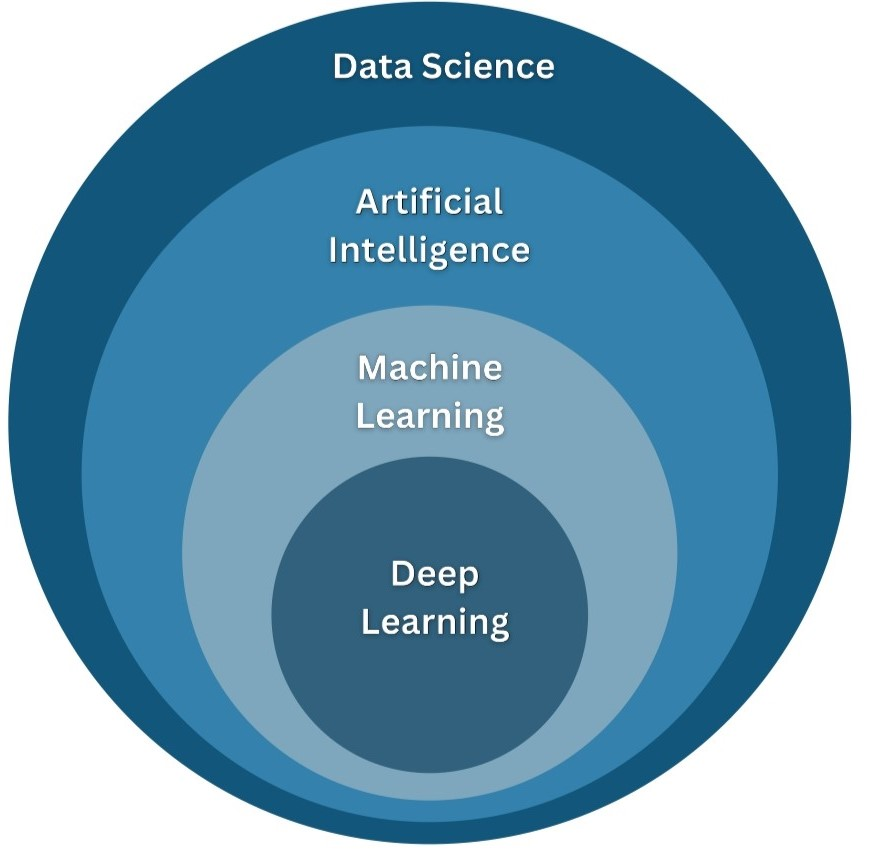
\includegraphics[width=0.4\textwidth]{img/ia.jpg}
    \caption{Relación entre Ciencia de Datos, Inteligencia Artificial, Machine Learning y Deep Learning.}
    \label{fig: ia}
\end{figure}


\section{Aprendizaje Automático}

Dentro de la inteligencia artificill Aprendizaje Automático (ML, por sus siglas en inglés) es la ciencia o el arte de programar ordenadores para que puedan aprender a partir de datos. Arthur Samuel lo definió en 1959 como ``el campo de estudio que otorga a las computadoras la capacidad de aprender sin ser explícitamente programadas''. Más formalmente, según Tom Mitchell (1997), ``se dice que un programa de computadora aprende de la experiencia \(E\) con respecto a alguna tarea \(T\) y alguna medida de rendimiento \(P\), si su rendimiento en \(T\), medido por \(P\), mejora con la experiencia \(E\)'' \citep{geron2022hands}. El aprendizaje automático ha revolucionado numerosos campos, permitiendo a las máquinas realizar tareas que antes requerían intervención humana directa. Desde la conducción autónoma hasta el diagnóstico médico, las aplicaciones del aprendizaje automático son diversas. A diferencia de los métodos tradicionales de programación, donde se codifican reglas explícitas, el aprendizaje automático permite que los sistemas descubran patrones y relaciones directamente a partir de los datos, adaptándose y mejorando con el tiempo.



Un ejemplo de aprendizaje automático es un filtro de spam que, dado ejemplos de correos electrónicos de spam y ejemplos de correos electrónicos normales (no spam, también llamados ``ham''), puede aprender a marcar el spam \citep{geron2022hands}. Los ejemplos que el sistema utiliza para aprender se llaman el conjunto de entrenamiento. Cada ejemplo de entrenamiento se llama una instancia de entrenamiento (o muestra). En este caso, la tarea \(T\) es marcar el spam en los nuevos correos electrónicos, la experiencia \(E\) son los datos de entrenamiento, y la medida de rendimiento \(P\) podría ser la precisión del filtro.

Un filtro de spam utilizando técnicas tradicionales de programación, en primer lugar consideraría cómo se ve normalmente el spam, detectando palabras comunes u otros patrones como el nombre del remitente y escribiendo reglas para cada una de estas. Pero si los encargados de mandar el spam detectan que todos los correos que incluyen la palabra ``Para usted'' o  ``cuenta bancaria'' son rechazados, pueden modificar estas palabras por otras y así ser aceptados por el filtro. Luego un filtro de spam que utiliza técnicas tradicionales de programación necesitaría ser actualizado continuamente para detectar correos electrónicos spam. 

Por otro lado, un filtro de spam basado en técnicas de aprendizaje automático nota automáticamente que "Para ti" se ha vuelto inusualmente frecuente en el spam marcado por los usuarios, y comienza a marcarlos sin intervención humana \citep{geron2022hands}.


\bigskip

El \textbf{esquema global de aprendizaje} consta de tres módulos principales: el generador, el entrenamiento y la decisión. El generador proporciona entradas estructuradas, principalmente vectores con atributos de los datos, para su procesamiento. El entrenamiento ajusta los parámetros del modelo basándose en las salidas deseadas, y por último, la decisión asigna categorías a nuevas muestras de entrada utilizando los parámetros aprendidos durante el entrenamiento \citep{pajares2021aprendizaje}.

\bigskip

En cuanto a la \textbf{clasificación de los sistemas de aprendizaje} automático, se distinguen cuatro tipos principales: el aprendizaje supervisado, no supervisado, semisupervisado y por refuerzo.

Un aprendizaje se dice que es \textbf{supervisado} si todos los datos tienen asociados las salidas deseadas (también llamadas etiquetas). Es decir, para todo dato de entrada x se conoce su salida y, luego tenemos información necesaria para aprender de la función que los relaciona y = f(x). El aprendizaje supervisado busca estimar la función $\hat{f}$ tal que $\hat{f}$ sea una buena aproximación de la función $f$ que relaciona las entradas x con las salidas Y.

Un aprendizaje se dice que es \textbf{supervisado} si todos los datos tienen asociadas las salidas deseadas (también llamadas etiquetas). Es decir, para todo dato de entrada \( x \) se conoce su salida \( y \), de tal forma que para una función desconocida $f$ que relaciona ambas, $y=f(x)$. El objetivo del aprendizaje supervisado es estimar la función \( f \) con una función \( \hat{f} \) de tal forma que \( \hat{f} \) sea una buena aproximación de la función \( f \) que relaciona las entradas \( x \) con las salidas \( y \). Un ejemplo de aprendizaje supervisado puede ser el del filtro de spam ya que se entrena el modelo con los correos y con la etiqueta de si son spam o no. Otros ejemplos incluyen regresión lineal, regresión logística, árboles de decisión y redes neuronales \citep{geron2022hands}.


Un aprendizaje se dice que es \textbf{no supervisado} si, al contrario que el aprendizaje supervisado, los datos de entrenamiento no están etiquetados. De esta forma, el modelo tiene que aprender sin supervisión (tambíen llamado sin ``profesor''). El objetivo principal de este tipo de algoritmos se basa en el agrupamiento, detección de anomalías o reducción de dimensionalidad \citep{geron2022hands}. 


En el caso de encontrarnos ante un problema en el que tengamos datos tanto etiquetados como sin etiquetar, nos encontramos ante un tipo de \textbf{aprendizaje semisupervisado}, que se encuentra entre el supervisado y el no supervisado. Este tipo de aprendizaje suele darse en situaciones en las que obtener etiquetas de los datos puede ser muy costoso pero sin embargo obtener datos sin etiquetar no tanto. Un ejemplo podría ser la agrupación de fotos donde sale la misma persona en Google Photos. La parte no supervisada sería la de agrupación y la supervisada la de dar una etiqueta a cada grupo \citep{geron2022hands}.


Por último, está el \textbf{aprendizaje por refuerzo}, un tipo de aprendizaje un poco diferente a los otros tres.  El sistema de aprendizaje, llamado agente, observa el entorno, selecciona y realiza acciones para obtener recompensas a cambio (o penalizaciones en forma de recompensas negativas). Luego debe aprender por sí mismo cuál es la mejor estrategia, llamada política, para obtener la mayor recompensa con el tiempo. Una política define qué acción debe elegir el agente cuando se encuentra en una situación determinada. Por ejemplo, muchos robots implementan algoritmos de aprendizaje por refuerzo para aprender a andar \citep{geron2022hands}.






¿PONER O NO?
El aprendizaje automático es excelente para:

\begin{itemize}
\item Problemas para los cuales las soluciones existentes requieren muchos ajustes o largas listas de reglas: un algoritmo de aprendizaje automático a menudo puede simplificar el código y funcionar mejor que el enfoque tradicional.

\item Problemas complejos para los que el enfoque tradicional no ofrece una buena solución: las mejores técnicas de Machine Learning quizás puedan encontrar una solución.

\item Entornos fluctuantes: un sistema de Machine Learning puede adaptarse a nuevos datos.

\item Obtener información sobre problemas complejos y grandes cantidades de datos.
\end{itemize}


\section{Aprendizaje profundo}

Dentro del Machine Learning, se encuentra el Deep Learning, cuya base son las redes neuronales artificiales (ANN). Las ANN son unas estructuras versátiles, potentes y escalables, lo que las hace ideales para abordar tareas grandes y complicadas para el aprendizaje profundo. Según \citep{pajares2021aprendizaje}, se definen como un modelo matemático inspirado en la estructura de una red neuronal biológica. Consiste en una red de neuronas interconectadas organizadas por capas, con una capa de entrada, una o más capas ocultas y una capa de salida \citep{dolling2002artificial}. En cada neurona se aplica una suma ponderada de las señales recibidas a las que se le aplica una función de activación o conexión no lineal. La capa de entrada recibe la información del exterior y la agrupa en la capa de entrada, mandando una salida a la siguiente capa a través de sus neuronas con \textbf{pesos} asociados en cada conexión. Las capas ocultas reciben información de otras neuronas artificiales y cuyas señales de entrada y salida permanecen dentro de la red. Por último, la capa de salida recibe la información procesada y la devuelve al exterior con la salida predicha por nuestro modelo. Además de los pesos que se van ajustando durante el entrenamiento, también está el \textbf{sesgo o bias}, que es un valor que se asigna a cada neurona de cada capa para añadir características adicionales a la red neuronal que antes no tenía. 


\subsection{Perceptrón}

Antes de profundizar en los modelos de redes neuronales más complejos y profundos, veamos el funcionamiento del modelo de ANN más simple, el \textit{perceptrón}. Este modelo es la base del resto de modelos de aprendizaje automático. Consiste en una capa de entrada y en una de salida en la que hay que aplicar dos etapas. En la figura \ref{img: perceptron} podemos ver el esquema para dos posibles salidas.

\begin{figure}[h!]
    \centering
    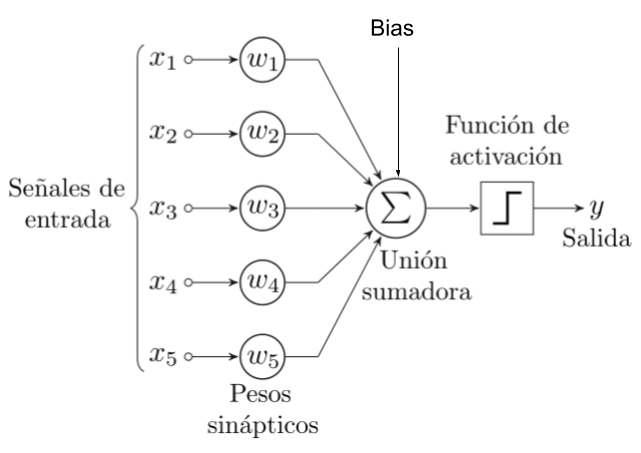
\includegraphics[width=0.4\textwidth]{img/perceptron.png}
    \caption{Modelo del perceptrón simple}
    \label{img: perceptron}
\end{figure}

La primera etapa del proceso consiste en calcular la suma promediada de sus entrada mediante una función lineal
\begin{equation}
f(x) = \sum_{i=1}^{n} w_i \cdot x_i + b
\end{equation}
Los coeficientes $w_i$, $i=1,2, \ldots, n$ llamados pesos, dan un valor determinado a cada una de las entradas en función de la importancia para obtener la salida. Además, el coeficiente $b$ es el sesgo o bias que se añade a la función. Otra forma práctica de escribir esta ecuación sería: $f(x) = \sum_{i=1}^{n} (w_i \cdot x_i) + b= w^t \cdot x + b$  donde $w^t = (w_1, \ldots, w_n)$ y $x^t = (x_1, \ldots, x_n)$

La segunda capa consiste en transformar la salida de la primera etapa mediante una función de activación. Se podría generalizar de la siguiente manera:
\begin{equation}
y = \phi(w^t \cdot x + b)
\end{equation}

Pero, ¿cómo ajusta los parámetros el perceptrón? El algoritmo de entrenamiento del perceptrón se basa en la regla de aprendizaje de Hebb y tiene en cuenta el error cometido por la red al hacer una predicción. El perceptrón se alimenta con una entrada de entrenamiento a la vez, y para cada una, realiza sus predicciones. Para cada neurona de salida que produce una predicción errónea, se refuerzan los pesos de conexión desde las entradas que habrían contribuido a la predicción correcta \citep{geron2022hands}. La regla se muestra en la Ecuación \ref{eq:perceptron_learning_rule}.

\begin{equation}
w_{i,j}^{(t+1)} = w_{i,j}^{(t)} + \eta (y_j - \hat{y_j}) x_i
\label{eq:perceptron_learning_rule}
\end{equation}

En esta ecuación, $w_{i,j}^{(t+1)}$ es el peso de conexión actualizado entre la $i$-ésima neurona de entrada y la $j$-ésima neurona de salida, $w_{i,j}^{(t)}$ es el peso de conexión actual entre la $i$-ésima neurona de entrada y la $j$-ésima neurona de salida, $x_i$ es el valor de la $i$-ésima entrada de la instancia de entrenamiento actual, $\hat{y_j}$ es la salida de la $j$-ésima neurona de salida, $y_j$ es la salida objetivo de la $j$-ésima neurona de salida y $\eta$ es la tasa de aprendizaje \citep{geron2022hands}.


El límite de decisión de cada neurona de salida es lineal, por lo que los perceptrones son incapaces de aprender patrones complejos. Esto significa que solo pueden separar los datos si hay una línea recta (o un hiperplano en dimensiones superiores) que divida las distintas clases de datos. Sin embargo, si las instancias de entrenamiento son linealmente separables, Rosenblatt demostró que este algoritmo convergería a una solución, es decir, encontraría un conjunto de pesos que clasifique correctamente todas las instancias de entrenamiento \citep{geron2022hands}. Esto se conoce como el Teorema de Convergencia del Perceptrón.



\subsection{El Perceptrón Multicapa y la Retropropagación}

Un Perceptrón Multicapa (MLP) está compuesto por una capa de entrada, una o más capas ocultas, y una capa final llamada capa de salida. Todas las capas, excepto la capa de salida, incluyen una neurona de sesgo y están completamente conectadas a la siguiente capa \citep{geron2022hands}.

Cuando una red neuronal artificial (ANN) contiene un conjunto profundo de capas ocultas\footnote{Se suele considerar más de dos capas oculatas como un conjunto profundo de capas ocultas}, se 
\begin{minipage}{0.54\textwidth}
llama red neuronal profunda (DNN). El campo del Aprendizaje Profundo estudia las DNNs, y más generalmente modelos que contienen conjuntos profundos de cálculos. Sin embargo, muchas personas hablan de Aprendizaje Profundo siempre que están involucradas redes neuronales.

\bigskip

David Rumelhart, Geoffrey Hinton y Ronald Williams publicaron un artículo revolucionario que introdujo el algoritmo de entrenamiento de retropropagación, que todavía se usa hoy en día. Consiste en un Descenso de Gradiente que utiliza una técnica eficiente para calcular los gradientes automáticamente. En solo dos etapas (una hacia adelante, una hacia atrás), el algoritmo de retropropagación puede determinar cómo se deben ajustar cada peso de conexión y cada término de sesgo para reducir el error. Para ello, calcula los gradientes del erro y a continuación, simplemente realiza un paso regular de Descenso de Gradiente, y todo el proceso se repite hasta que la red converge a la solución.

\end{minipage}
\begin{minipage}{0.05\textwidth}
\textbf{ }
\end{minipage}
\begin{minipage}{0.4\textwidth}
	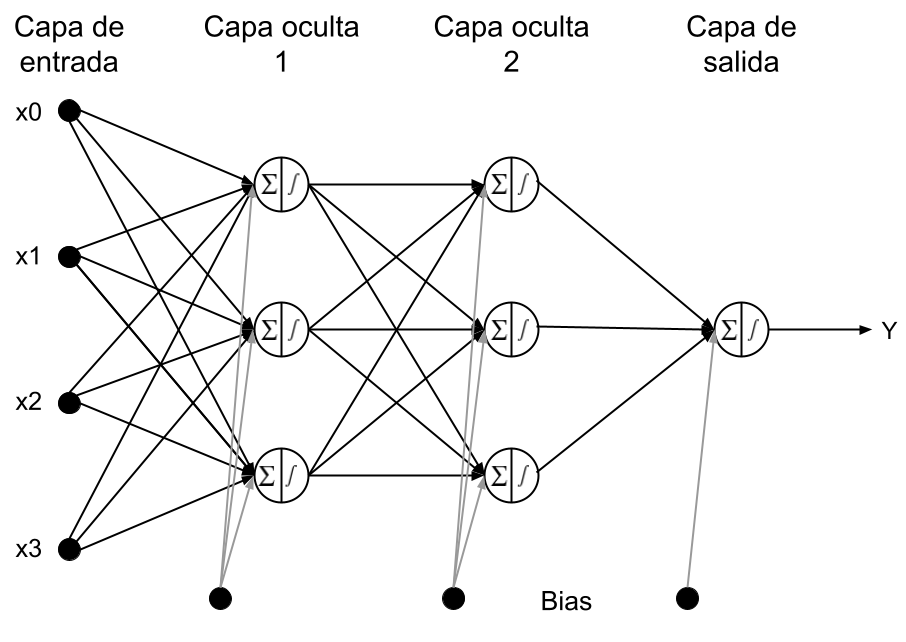
\includegraphics[width=1.1\textwidth]{img/multicapa}
	\captionof{figure}{Arquitectura de un Perceptrón Multicapa con tres entradas, dos capas ocultas de tres neuronas cada una y una neurona de salida (las neuronas de sesgo se muestran aquí, pero normalmente son implícitas).}
	\label{fig:mlp_architecture}
\end{minipage}

El algoritmo maneja un mini-lote a la vez (batch size), y pasa por el conjunto completo de entrenamiento múltiples veces. Cada pasada se llama época (epoch). Cada mini-lote se pasa a la capa de entrada de la red, que lo envía a la primera capa oculta. El algoritmo luego calcula la salida de todas las neuronas en esta capa (para cada instancia en el mini-lote). El resultado se pasa a la siguiente capa, su salida se calcula y se pasa a la siguiente capa, y así sucesivamente hasta obtener la salida de la última capa, la capa de salida. Esta es la pasada hacia adelante: es exactamente como hacer predicciones, excepto que todos los resultados intermedios se preservan ya que son necesarios para la pasada hacia atrás. A continuación, el algoritmo mide el error de salida de la red (es decir, utiliza una función de pérdida que compara la salida deseada y la salida real de la red, y devuelve alguna medida del error). Luego, calcula cuánto contribuyó cada conexión de salida al error. Esto se hace analíticamente aplicando la regla de la cadena, lo que hace que este paso sea rápido y preciso. El algoritmo luego mide cuánto de estas contribuciones de error provienen de cada conexión en la capa inferior, nuevamente utilizando la regla de la cadena, trabajando hacia atrás hasta que el algoritmo llega a la capa de entrada. Como se explicó anteriormente, esta pasada inversa mide eficientemente el gradiente de error en todos los pesos de conexión en la red propagando el gradiente de error hacia atrás a través de la red (de ahí el nombre del algoritmo). Finalmente, el algoritmo realiza un paso de Descenso de Gradiente para ajustar todos los pesos de conexión en la red, utilizando los gradientes de error que acaba de calcular \citep{geron2022hands}.

Este algoritmo es tan importante que vale la pena resumirlo nuevamente: para cada instancia de entrenamiento, el algoritmo de retropropagación primero hace una predicción (pasada hacia adelante) y mide el error, luego pasa por cada capa en reversa para medir la contribución del error de cada conexión (pasada hacia atrás), y finalmente ajusta los pesos de conexión para reducir el error (paso de Descenso de Gradiente).

Es importante inicializar aleatoriamente todos los pesos de conexión de las capas ocultas, de lo contrario, el entrenamiento fallará. Por ejemplo, si inicializas todos los pesos y sesgos a cero, entonces todas las neuronas en una capa dada serán perfectamente idénticas, y por lo tanto la retropropagación las afectará de la misma manera, por lo que permanecerán idénticas. En otras palabras, a pesar de tener cientos de neuronas por capa, tu modelo actuará como si tuviera solo una neurona por capa: no será muy inteligente. Si en cambio inicializas aleatoriamente los pesos, rompes la simetría y permites que la retropropagación entrene un equipo diverso de neuronas \citep{geron2022hands}.



\section{Optimización del modelo} MEJOR CONEXIÓN DE INTRODUCCIÓN

La optimización consiste en minimizar o maximizar una función $f(\mathbf{x})$ modificando $\mathbf{x}$. En general, la optimización hace referencia a una minimización, ya que la maximización es equivalente a la minimización de $-f(\mathbf{x})$. La función a minimizar se conoce como función objetivo, función de coste, función de pérdida o función de error. La función de pérdida calcula la discrepancia entre la salida de la red neuronal (predicción) y la etiqueta verdadera. Su objetivo es minimizar este error a lo largo del entrenamiento. A la función o grupo de funciones que se están minimizando se denominan \textit{loss functions}, y el valor mínimo se identifica mediante el símbolo $x* = \arg \min f(\mathbf{x})$ \citep{pajares2021aprendizaje}. 

Se sabe de Cálculo Diferencial que la derivada de una función en un punto $x$ calcula la pendiente de la función en dicho punto. Sea $\delta$ un valor, entonces se tiene que $f(x + \delta) \approx f(x) + f'(x)\delta$, es decir, un pequeño cambio en la entrada permite aproximar su valor en la salida gracias a la derivada de la función. Para poder utilizar esta aproximación, es necesario que la función sea diferenciable \footnote{En la red neuronal se realizan cálculos en cada capa y si estos cálculos son diferenciables, la función de pérdida también lo será. Sin embargo, a veces se usan funciones de activación como ReLU, que no son diferenciables en todos los puntos. En estos casos, se debe aplicar una aproximación de la derivada para poder utilizar la función en el método de descenso de gradiente.}. Este método se conoce como descenso de gradiente (\textit{gradient descent}). Durante este método, se propaga el error hacia atrás a través de la estructura del modelo, de forma que los pesos en las redes neuronales vayan ajustándose a lo largo del entrenamiento. Esto cierra el ciclo de aprendizaje entre el envío de los datos hacia adelante, la generación de predicciones y la mejora durante la propagación hacia atrás. Al adaptar los pesos, el modelo probablemente mejore (a veces mucho, a veces ligeramente) y, por lo tanto, se dice que se ha realizado el aprendizaje \citep{pajares2021aprendizaje}. 

\subsection{Descenso de gradiente}


Sea $f: S \in \mathbb{R}^n \to \mathbb{R}^m$, donde $n$ y $m$ son enteros. Cuando $f'(x) = 0$, la derivada no proporciona información sobre la dirección en la que hay que moverse. De esta forma, los puntos con $f'(x) = 0$ se conocen como puntos críticos o puntos estacionarios. Un punto $x_0$ es un \textbf{mínimo local} si $\exists \epsilon$ tal que $f(x_0) \leq f(x)$ para todo $x \in B(x_0, \epsilon)$\footnote{$B(a,b)$ hace referencia a la bola o disco de centro $a$ y radio $b$}. Por otra parte, un punto \( x_0 \) es un \textbf{punto de inflexión} de la función \( f \) si \( f \) es continua en \( x_0 \) y existe un entorno \( B(x_0, \epsilon) \) tal que \( f'' \) cambia de signo en \( x_0 \). Esto implica que en un lado de \( x_0 \),  \( f''(x) \) es positiva y en el otro lado es negativa, o viceversa. Si un punto $x_0$ cumple que $\exists \epsilon$ tal que $f(x_0) \leq f(x)$ para todo $x \in S$, entonces $x_0$ es un \textbf{mínimo global}. Puede haber solo un mínimo global o múltiples mínimos globales de la función. También es posible que haya mínimos locales que no sean globalmente óptimos. En el contexto del aprendizaje automático, se optimizan funciones que pueden tener muchos mínimos locales que no son óptimos y muchos puntos de inflexión rodeados de regiones muy planas. Todo esto hace que la optimización sea difícil, especialmente cuando la entrada a la función es multidimensional. Por lo tanto, se suele conformar con encontrar un valor que sea muy bajo pero no necesariamente mínimo en ningún sentido formal \citep{pajares2021aprendizaje}.


A menudo es necesario minimizar funciones que tienen múltiples ($n$) entradas: $f : \mathbb{R}^n \to \mathbb{R}$, con una única salida. Con múltiples entradas, se debe utilizar el concepto de derivadas parciales $\frac{\partial f}{\partial x_i}$, que mide cómo cambia $f$ según aumenta la variable $x_i$, en el punto $\mathbf{x}$. El gradiente de $f$ es el vector que contiene todas las derivadas parciales, denotado por $\nabla f(\mathbf{x})$. En múltiples dimensiones, los puntos críticos son puntos en los que cada elemento del gradiente es igual a cero. La derivada direccional en la dirección $\mathbf{u}$ (vector unitario) es la pendiente de la función $f$ en esa dirección $\mathbf{u}$. En otras palabras, la derivada direccional es la derivada de la función $f(\mathbf{x} + \alpha \mathbf{u})$ con respecto a $\alpha$, evaluada en $\alpha = 0$. Usando la regla de la cadena, se determina que $f(\mathbf{x} + \alpha \mathbf{u})$ evalúa $\mathbf{u} \cdot \nabla f(\mathbf{x})$ cuando $\alpha = 0$ \citep{pajares2021aprendizaje}.

Para minimizar $f$, es deseable encontrar la dirección en la que $f$ disminuye de forma más rápida, lo que se puede hacer usando la derivada direccional:
\begin{equation}
    \min_{\mathbf{u}} D_{\mathbf{u}} f(\mathbf{x}) = \min_{\mathbf{u}} \nabla f(\mathbf{x}) \cdot \mathbf{u} = - \|\nabla f(\mathbf{x})\|,
\end{equation}
donde $\theta$ es el ángulo entre $\mathbf{u}$ y el gradiente. Sustituyendo $||u||_2 = 1$ e ignorando factores que no dependen de $u$, se concreta en minimizar $min_u \cos \theta$. Se puede hacer decrecer $f$ moviéndose en la dirección opuesta del gradiente, lo que se conoce como método del gradiente descendente por lotes (\textit{steepest descent} o \textit{gradient descent}), que propone un nuevo punto:
\begin{equation}
    \mathbf{x}' = \mathbf{x} - \eta \nabla f(\mathbf{x}),
\end{equation}
donde $\eta$ es la razón de aprendizaje (o \textit{learning rate}), que determina el tamaño del paso. En caso de aplicar esta ecuación a cada uno de los datos de entrada, se llamará \textbf{descenso de gradiente por lotes}. El learning rate se puede elegir de varias formas, una de ellas es fijarlo a un valor constante pequeño. Algunas veces se puede determinar la dimensión del paso que hace desaparecer la derivada direccional. Otra aproximación consiste en evaluar $f(\mathbf{x} - \eta \nabla f(\mathbf{x}))$ para varios valores de $\eta$ y escoger el que proporciona el valor de la función objetivo menor. Esta estrategia se denomina búsqueda en línea. El gradiente descendente converge cuando cada elemento del gradiente es cero o muy próximo a él \citep{pajares2021aprendizaje}.  Escoger valores de $\eta$ muy pequeños hace que la convergencia sea muy lenta. Sin embargo, valores muy grandes pueden hacer que el algoritmo diverja y se aleje en cada paso más del valor óptimo.

También esta la posibilidad de añadirle momentum al SGD, que es un hiperparámetro mayor o igual a 0 que acelera el descenso del gradiente en la dirección relevante y amortigua las oscilaciones. Su valor por defecto es 0. 

\subsection{Descenso de gradiente estocástico}


El Descenso de Gradiente Estocástico (SGD, por sus siglas en inglés) es un algoritmo utilizado para minimizar una función objetivo en problemas de aprendizaje automático. 
\[
w^{(t+1)} = w^{(t)} - \eta \nabla J_i (w^{(t)})
\]
donde $w$ son los pesos que desean estimarse en cada iteración y $J_i$ es la i-ésima observación del conjunto de datos. El SGD selecciona aleatoriamente una elemento del conjunto de entrenamiento en cada iteración y calcula los gradientes basándose únicamente en esa instancia individual \citep{pajares2021aprendizaje}. Esto hace que el algoritmo sea mucho más rápido que calculándolo para todos los datos, debido a que en cada iteración solo se necesita manipular una pequeña cantidad de datos. Además, permite entrenar con conjuntos de datos muy grandes. Sin embargo, debido a su naturaleza aleatoria, el SGD es mucho menos regular que el Descenso de Gradiente por Lote. En lugar de disminuir suavemente hasta alcanzar el mínimo, la función de perdida oscilará, disminuyendo solo en promedio. Con el tiempo, el algoritmo se acercará mucho al mínimo, pero continuará oscilando alrededor de él sin asentarse completamente \citep{geron2022hands}.

Una solución a este problema es reducir gradualmente la tasa de aprendizaje. Al principio, los pasos son grandes, lo que ayuda a hacer un progreso rápido y a escapar de mínimos locales. Luego, los pasos se hacen más pequeños, permitiendo que el algoritmo se asiente en el mínimo global \citep{geron2022hands}.


Los pasos de este método de optimización son: Primero, se elige un vector inicial de parámetros \( w \) (que puede ser seleccionado aleatoriamente) y una razón de aprendizaje \( \eta \). Los siguientes pasos se repiten hasta que se consiga un mínimo aproximado. En cada iteración, se seleccionan aleatoriamente ejemplos del conjunto de entrenamiento. Para cada ejemplo \( i = 1, 2, \ldots, n \), se actualiza el vector de parámetros utilizando la fórmula \( w^{(t+1)} = w^{(t)} - \eta \nabla J_i (w^{(t)}) \) \citep{pajares2021aprendizaje}.


\subsection{Descenso de gradiente por mini-lotes}


El Descenso de Gradiente por Mini-lote (Mini-batch Gradient Descent) es un algoritmo que combina aspectos del Descenso de Gradiente por Lote y el SGD (Stochastic Gradient Descent). A diferencia de estos métodos, en lugar de calcular los gradientes basándose en todo el conjunto de entrenamiento o en una única instancia, el Descenso de Gradiente por Mini-lote calcula los gradientes basándose en pequeños subconjuntos aleatorios de instancias llamados mini-lotes (mini-batch). Estos subconjuntos definen el número de muestras utilizadas antes de actualizar los pesos de la red en el modelo. Si se utilizan todas las muestras de entrenamiento para crear un lote, se denomina \textbf{descenso del gradiente por lotes}. Si el lote tiene el tamaño de una muestra, se llama \textbf{descenso de gradiente estocástico}. Cuando el lote tiene más de una muestra pero es menor que el tamaño del conjunto de datos de entrenamiento, se denomina \textbf{descenso de gradiente de mini-lote}. Este enfoque logra un progreso menos errático que el SGD, especialmente con mini-lotes relativamente grandes, y se acerca más al mínimo, aunque puede ser más difícil escapar de mínimos locales. No obstante, con un buen plan de aprendizaje, tanto el SGD como el Descenso de Gradiente por Mini-lote pueden llegar al mínimo \citep{geron2022hands}.

Otro parámetro relevante es la \textbf{época (epoch)}, que define cuántas veces el conjunto total de muestras es procesado por el algoritmo. Cada muestra del conjunto \(N\) tiene una oportunidad de actualizar los pesos en cada epoch. Una epoch puede contener uno o más lotes. Para mayor claridad, se puede pensar en un bucle sobre el número de epochs, donde cada iteración opera sobre \(N\). Dentro de esta iteración, existe otra iteración anidada que actúa sobre cada lote de muestras. El número de epochs varía según el tipo de datos y puede ser alto, como 10, 100, 1000 o más, garantizando una eficiencia suficiente, aunque también puede ser menor \citep{pajares2021aprendizaje}.


\subsection{Propagación de la raíz Media Cuadrada}

Además de estos métodos, existen optimizadores avanzados que mejoran la eficiencia del entrenamiento. Entre ellos se encuentra la \textbf{Propagación de la Raíz Media Cuadrática (RMSProp)}. Este método adapta la tasa de aprendizaje para cada parámetro manteniendo una media móvil de los cuadrados de los gradientes. La actualización del parámetro \(w(t)\) se realiza de la siguiente manera \citep{pajares2021aprendizaje}:

\[
v(t) = \beta v(t-1) + (1-\beta) (g(t))^2
\]

\[
w(t) = w(t-1) - \frac{\eta}{\sqrt{v(t) + \epsilon}} g(t)
\]

donde \(\beta\) es el factor de decaimiento de la media, \(\eta\) es la tasa de aprendizaje y \(\epsilon\) es una constante pequeña para evitar divisiones por cero \citep{pajares2021aprendizaje}.




\subsection{Estimación del Momento Adaptativo}

Otro optimizador relevante es \textbf{Adam (Adaptive Moment Estimation)}, que combina las ideas de RMSProp con el momento. Adam mantiene medias móviles de los gradientes y de los cuadrados de los gradientes. Las actualizaciones de los parámetros se realizan de la siguiente manera \citep{pajares2021aprendizaje}:

\[
m(t) = \beta_1 m(t-1) + (1-\beta_1) g(t)
\]

\[
v(t) = \beta_2 v(t-1) + (1-\beta_2) (g(t))^2
\]

\[
\hat{m}(t) = \frac{m(t)}{1 - \beta_1^t}
\]

\[
\hat{v}(t) = \frac{v(t)}{1 - \beta_2^t}
\]

\[
w(t) = w(t-1) - \frac{\eta \hat{m}(t)}{\sqrt{\hat{v}(t)} + \epsilon}
\]

donde \(\beta_1\) y \(\beta_2\) son factores de decaimiento de las medias, \(\eta\) es la tasa de aprendizaje y \(\epsilon\) es una constante pequeña para evitar divisiones por cero \citep{pajares2021aprendizaje}.












\section{Función de activación.}

Entre capa y capa de las redes neuronales, cada neurona suma ponderadamente las entradas provenientes de las neuronas de la capa anterior. Este resultado, se lo pasa a una función no lineal, llamada función de activación, que permiten que la red neuronal pueda aprender, representar patrones complejos y crear relaciones no lineales entre las características de entrada y la salida. El valor resultante de aplicarle la función es el valor que se le queda asociado a esta neurona, para que futuras capas puedan usarlo. En esta sección, describimos varias funciones de activación populares, sus propiedades y aplicaciones \citep{pajares2021aprendizaje}.


\subsubsection*{Softmax}


La función \textbf{Softmax} se utiliza comúnmente en la capa de salida de redes neuronales para problemas de clasificación multiclase. Convierte un vector de valores arbitrarios en un vector de probabilidades, donde la suma de todas las probabilidades es 1. La función Softmax está definida como:

\begin{equation}
    \text{Softmax}(z_i) = \frac{e^{z_i}}{\sum_{j=1}^{K} e^{z_j}}
\end{equation}

donde \(z_i\) es el valor de la \(i\)-ésima neurona de salida, y \(K\) es el número total de clases. La interpretación de esta función es que transforma las salidas en probabilidades, facilitando la toma de decisiones sobre la clase a la que pertenece una muestra en función de las probabilidades más altas \citep{pajares2021aprendizaje}. 




\subsubsection*{Sigmoide}


\begin{minipage}{0.6\textwidth}
    La función \textbf{sigmoide}, también conocida como la función logística, convierte entradas en el rango \(0, 1\). Está definida como:
\begin{equation}
    \sigma(x) = \frac{1}{1 + e^{-x}} 
\end{equation}
Sin embargo, tiene problemas como la saturación del gradiente (cuando los valores se aproximan a 0 o 1, el gradiente tiende a 0, lo que afecta en la actualización de los pesos) o los pesos tienen esperanza de la función de salida positiva, lo que puede llevar a una convergencia lenta \citep{pajares2021aprendizaje}.
\end{minipage}
\begin{minipage}{0.05\textwidth}
\textbf{ }
\end{minipage}
\begin{minipage}{0.35\textwidth}
    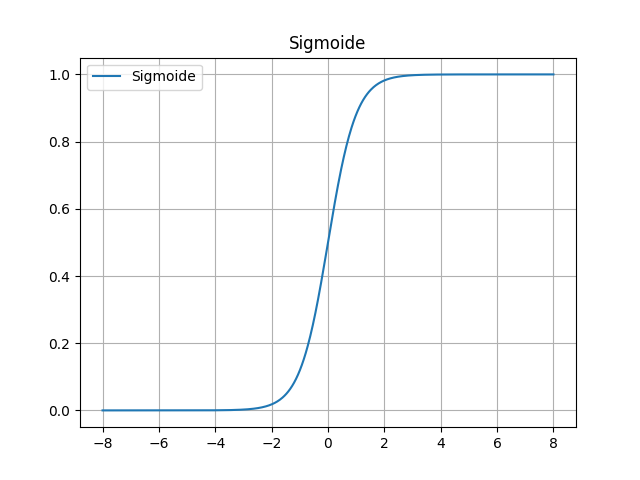
\includegraphics[width=1.1\textwidth]{img/Sigmoide.png}
    \captionof{figure}{Gráfica de la función sigmoide.}
    \label{img: sigmoide}
\end{minipage}



\subsubsection*{Sigmoide dura}


\begin{minipage}{0.35\textwidth}
    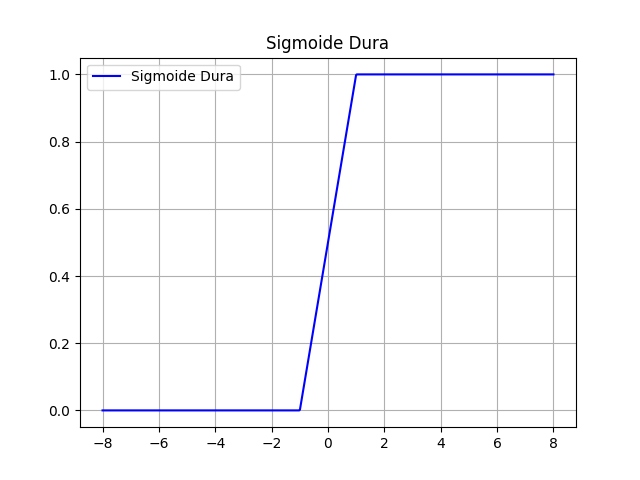
\includegraphics[width=1.1\textwidth]{img/Sigmoide Dura.png}
    \captionof{figure}{Gráfica de la función sigmoide dura.}
    \label{img: sigmoideDura}
\end{minipage}
\begin{minipage}{0.05\textwidth}
\textbf{ }
\end{minipage}
\begin{minipage}{0.6\textwidth}
    Para solucionar el problema de la saturación del gradiente en los extremos, está la función \textbf{sigmoide dura} (\textit{hard-sigmoid}), que es una aproximación simplificada de la función sigmoide. Su fórmula es la siguiente:

\begin{equation}
    f(x) = \max(0, \min(1, \frac{x+1}{2}))
\end{equation}

Esta función es computacionalmente más eficiente y evita los problemas de saturación en los extremos \citep{pajares2021aprendizaje}.
\end{minipage}



\subsubsection*{Función Tangente hiperbólica}
 

\begin{minipage}{0.6\textwidth}
    La función \textbf{tangente hiperbólica (tanh)} es similar a la sigmoide pero escala las salidas al rango \([-1, 1]\):

\begin{equation}
    \tanh(x) = \frac{\sinh(x)}{\cosh(x)} = \frac{e^x + e^{-x}}{e^x + e^{-x}}
\end{equation}

Aunque también sufre de saturación del gradiente, \textit{tanh} centra las salidas alrededor de cero, lo que puede acelerar el entrenamiento \citep{pajares2021aprendizaje}. 
\end{minipage}
\begin{minipage}{0.05\textwidth}
\textbf{ }
\end{minipage}
\begin{minipage}{0.35\textwidth}
    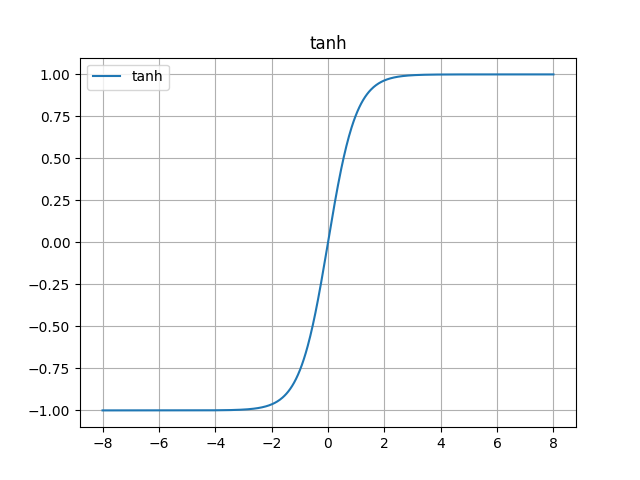
\includegraphics[width=1.1\textwidth]{img/tanh.png}
    \captionof{figure}{Gráfica de la función tangente hiperbólica.}
    \label{img: tanh}
\end{minipage}



\subsubsection*{Función ReLU}

\begin{minipage}{0.35\textwidth}
    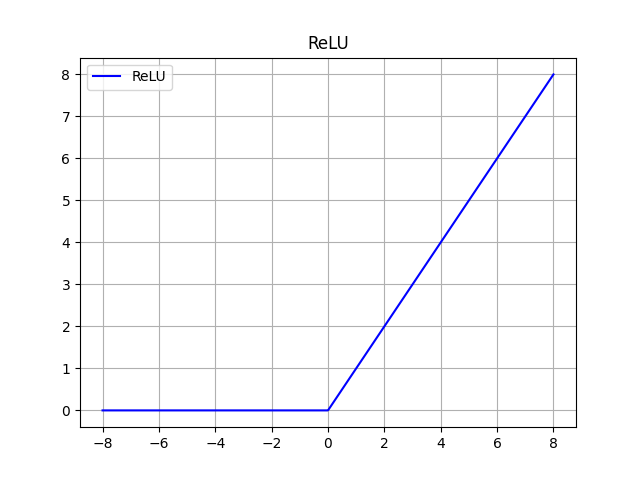
\includegraphics[width=1.1\textwidth]{img/ReLU.png}
    \captionof{figure}{Gráfica de la función ReLU.}
    \label{img: relu}
\end{minipage}
\begin{minipage}{0.05\textwidth}
\textbf{ }
\end{minipage}
\begin{minipage}{0.6\textwidth}
    La \textbf{función ReLU} es popular debido a su simplicidad y efectividad para solventar el problema de la saturación del gradiente.

\begin{equation}
    f(x) = \max(0, x)
\end{equation}
Sin embargo, la función ReLU tiene algunos problemas, como el problema de la ``ReLU muerta'' \citep{maas2013rectifier} y la falta de diferenciabilidad en cero. Para este problema último, se suele asignar un valor arbitrario para este valor como 0, 0.5 o 1 citep{pajares2021aprendizaje}. Esto ocurre cuando se aprende un sesgo negativo grande, haciendo que la salida de la neurona sea siempre cero, sin importar la entrada \citep{apicella2021survey}. Por eso, a continuación, discutimos algunas variantes de ReLU.
\end{minipage}


\subsubsection*{Función Leaky ReLU (LReLU)}

\begin{minipage}{0.6\textwidth}
    Una de las primeras funciones de activación basadas en ReLU fue \textbf{LReLU} \citep{maas2013rectifier}. La función LReLU fue un intento de aliviar los problemas potenciales de ReLU mencionados anteriormente. Se define como:

\begin{equation}
    f(x) = \max(0.001x, x)
\end{equation}

La función de activación Leaky ReLU permite que la neurona tenga un pequeño gradiente cuando su salida es cero o negativa (es decir, cuando $x \leq 0)$. Sin embargo, se ha demostrado que Leaky ReLU funciona de manera casi idéntica a la ReLU original, por lo que no mejora significativamente el rendimiento de la red. Además, se propuso una versión aleatoria de ReLU, donde el valor de $x$ se elige aleatoriamente de una distribución uniforme \( U(l, u) \) con \( 0 \le l < u < 1 \) \citep{apicella2021survey}.
\end{minipage}
\begin{minipage}{0.05\textwidth}
\textbf{ }
\end{minipage}
\begin{minipage}{0.35\textwidth}
    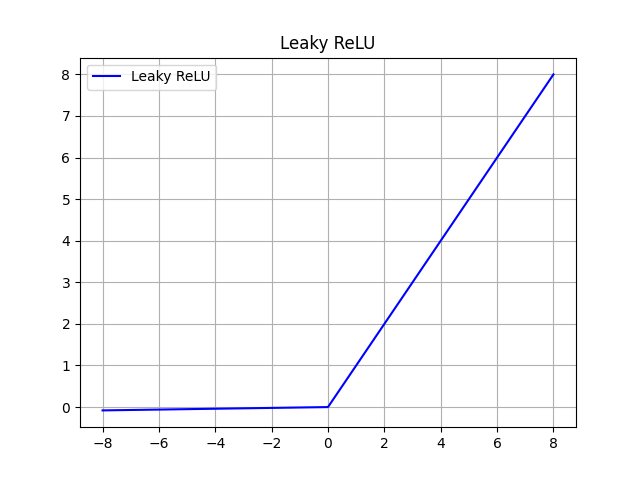
\includegraphics[width=1.1\textwidth]{img/Leaky ReLU.png}
    \captionof{figure}{Gráfica de la función Leaky ReLU.}
    \label{img: LReLU}
\end{minipage}


\subsubsection*{Función paramétrica ReLU(PReLU)}

\begin{minipage}{0.35\textwidth}
    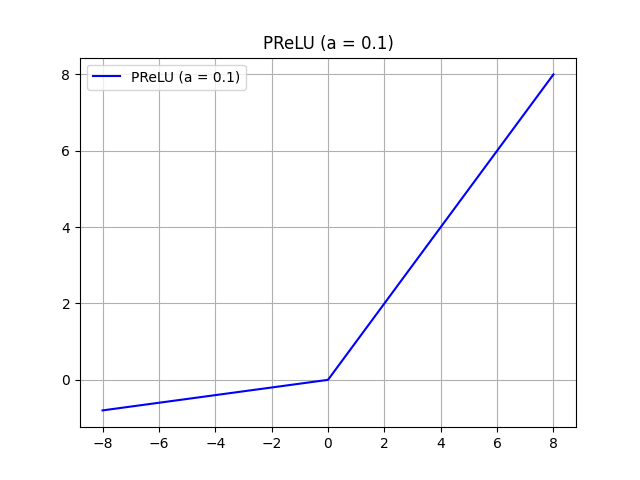
\includegraphics[width=1.1\textwidth]{img/PReLU.png}
    \captionof{figure}{Gráfica de la función Paramétrica ReLU.}
    \label{img: PReLU}
\end{minipage}
\begin{minipage}{0.05\textwidth}
\textbf{ }
\end{minipage}
\begin{minipage}{0.6\textwidth}
    Una forma de generalizar la función anterior es introduciendo un parámetro \(\alpha\) para ajustar la pendiente para entradas negativas. Esta función se llama PReLU y se define:
\begin{equation}
    f(x; \alpha) = 
    \begin{cases} 
      \alpha x & \text{si } x < 0 \\ 
      x & \text{si } x \geq 0 
    \end{cases}
    \label{eq:prelu}
\end{equation}
Cuando $\alpha = 0$, la función se corresponde con ReLU y cuando $\alpha > 0$, con la LReLU. La función se adapta durante el entrenamiento, permitiendo más flexibilidad que ReLU o LReLU. 
\end{minipage}

\subsubsection*{Función Softplus}

\begin{minipage}{0.6\textwidth}
    La función softplus puede considerarse una aproximación suave de la función ReLU. Se define como:
\begin{equation}
\text{softplus}(a) = \log(1 + \exp(a))
\end{equation}

La forma más suave de la función y la ausencia de puntos no diferenciables podrían sugerir un mejor comportamiento y un entrenamiento más fácil como función de activación. Sin embargo, los resultados experimentales obtenidos tienden a contradecir esta hipótesis, sugiriendo que las propiedades de ReLU pueden facilitar el entrenamiento supervisado mejor que las funciones softplus \citep{apicella2021survey}.
\end{minipage}
\begin{minipage}{0.05\textwidth}
\textbf{ }
\end{minipage}
\begin{minipage}{0.35\textwidth}
    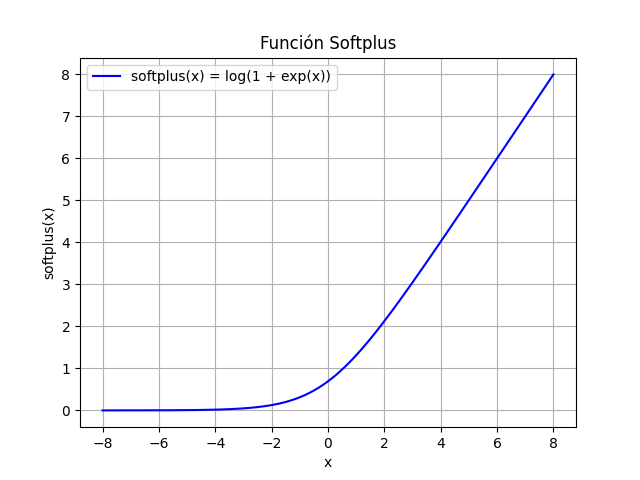
\includegraphics[width=1.1\textwidth]{img/softplus.png}
    \captionof{figure}{Gráfica de la función Softplus.}
    \label{img:softplus}
\end{minipage}


\subsubsection*{Función ELU}

\begin{minipage}{0.35\textwidth}
    \includegraphics[width=1.1\textwidth]{img/elu.png}
    \captionof{figure}{Gráfica de la función ELU.}
    \label{img:elu}
\end{minipage}
\begin{minipage}{0.05\textwidth}
\textbf{ }
\end{minipage}
\begin{minipage}{0.6\textwidth}
    La \textbf{función ELU} es una función de activación que mantiene la identidad para argumentos positivos pero con valores no nulos para los negativos. Se define como:
    \[
    \text{ELU}(a) =
    \begin{cases} 
    a & \text{si } a > 0 \\
    \alpha \cdot (\exp(a) - 1) & \text{de lo contrario}
    \end{cases}
    \]
    donde \( \alpha \) controla el valor para entradas negativas. Los valores dados por las unidades ELU empujan la media de las activaciones más cerca de cero, permitiendo una fase de aprendizaje más rápida, a costa de un hiperparámetro extra (\( \alpha \)) que necesita ser establecido durante el entrenamiento \citep{apicella2021survey}.
\end{minipage}


\subsubsection*{Funciones Swish y SiLU}

\textbf{Swish y SiLU} combinan la función sigmoide con otros parámetros para proporcionar una activación suave y no lineal. Ambas funciones se han probado en tareas de aprendizaje por refuerzo y en otros contextos, demostrando su efectividad \citep{apicella2021survey}.

\begin{equation}
    \text{SiLU}(a) = a \cdot \sigma(a) = \frac{a}{1 + e^{-a}}
\end{equation}

La derivada de SiLU se define como:

\begin{equation}
    \text{dSiLU}(a) = \sigma(a) \left( 1 + a (1 - \sigma(a)) \right)
\end{equation}

Donde \(\sigma(a)\) es la función sigmoide.

La función Swish se define de manera similar, pero con un parámetro adicional \(\beta\):
\begin{equation}
    \text{Swish}(x) = x \cdot \sigma(\beta x) = \frac{x}{1 + e^{-\beta x}}
\end{equation}

Para \(\beta = 1\), Swish es equivalente a SiLU. La Figura \ref{fig:activf} muestra las gráficas de las funciones Swish (con \(\beta = 3\)) y SiLU.

\begin{figure}[h]
    \centering
    \begin{minipage}[b]{0.45\textwidth}
        \centering
        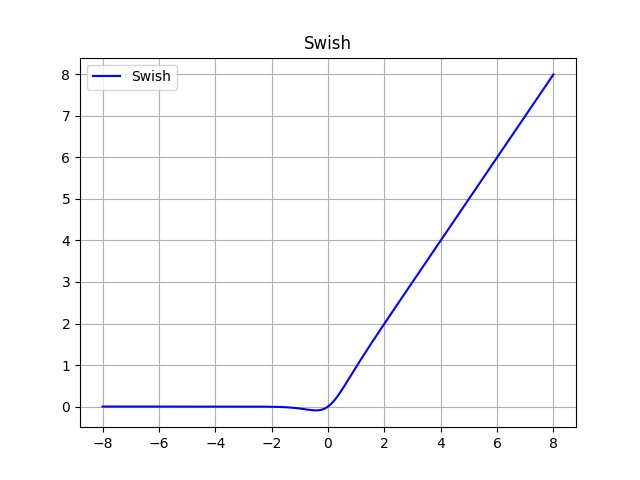
\includegraphics[width=\textwidth]{img/Swish.png}
        \caption{Gráfica de la función Swish con \(\beta = 3\).}
        \label{fig:swish}
    \end{minipage}
    \hfill
    \begin{minipage}[b]{0.45\textwidth}
        \centering
        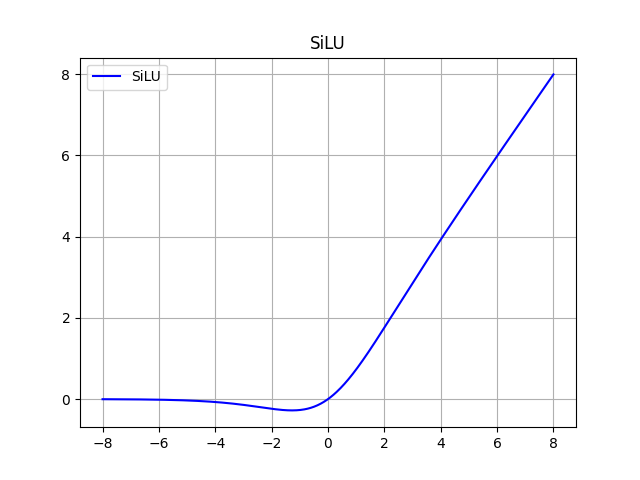
\includegraphics[width=\textwidth]{img/SiLU.png}
        \caption{Gráfica de la función SiLU.}
        \label{fig:silu}
    \end{minipage}
    \caption{Comparación de las funciones de activación Swish y SiLU.}
    \label{fig:activf}
\end{figure}



Las funciones de activación juegan un papel esencial en la formación de redes neuronales al permitir que las redes aprendan y generen relaciones complejas. Desde funciones clásicas como la sigmoide y tanh, hasta variantes más recientes como ReLU, LReLU y ELU, cada función tiene sus propios beneficios y limitaciones. La elección de la función de activación depende del tipo de problema al que nos enfrentemos y de lo que se busque con el modelo, pero tiene que ser una elección acertada, ya que puede influir significativamente en el rendimiento del modelo. Además, permiten resolver el desvanecimiento del gradiente durante el proceso de aprendizaje, evitando que el gradiente se acerque a cero, cumpliendo la hipótesis de derivabilidad \citep{pajares2021aprendizaje}.


\section{Función de perdida}

En el aprendizaje supervisado, las funciones de pérdida son herramientas muy importantes para evaluar qué tan bien un modelo predice los resultados esperados. Su objetivo es cuantificar el grado de error en las predicciones realizadas por el modelo, lo cual es fundamental para el ajuste de sus parámetros durante el entrenamiento. En términos generales, estas funciones se dividen en dos grandes categorías: las utilizadas para problemas de clasificación y las utilizadas para problemas de regresión \citep{pajares2021aprendizaje}. Ambas buscan minimizar el error, pero lo hacen con diferentes enfoques dependiendo de la naturaleza de la variable de salida.

\subsection{Clasificación}

En los problemas de clasificación, la tarea del modelo es asignar una etiqueta a cada observación basada en las características de entrada. La etiqueta es una variable categórica que indica a cuál de varias categorías pertenece cada observación. Las funciones de pérdida en clasificación miden la discrepancia entre las etiquetas reales y las etiquetas predichas, o las probabilidades de las categorías predichas.

\subsubsection{Entropía Cruzada}

La entropía cruzada mide la diferencia entre la distribución de probabilidad verdadera de las etiquetas y la distribución de probabilidad predicha por el modelo. Existen dos variantes principales:

\begin{itemize}
	\item La \textbf{entropía cruzada categórica} se utiliza cuando se predicen múltiples categorías (multiclase). Se calcula como:

	\begin{equation}
    		H(p, q) = -\sum_{x} p(x) \log q(x)
	\end{equation}

	Aquí, \(p(x)\) es la distribución verdadera (generalmente representada como \textit{one-hot} para una categoría) y \(q(x)\) es la distribución predicha. Esta función penaliza las predicciones que se desvían de las probabilidades verdaderas, con valores más altos indicando mayores discrepancias \citep{pajares2021aprendizaje}. 

	\item La\textbf{ entropía cruzada binaria} se aplica a problemas de clasificación binaria, donde solo hay dos posibles etiquetas. Se define como:

	\begin{equation}
    		H(p, q) = - \left[ p \log q + (1 - p) \log (1 - q) \right]
	\end{equation}

	Aquí, \(p\) es la probabilidad de la etiqueta verdadera (1 para la clase positiva, 0 para la clase negativa), y \(q\) es la probabilidad predicha para la clase positiva. Esta variante es más sencilla y específica para problemas donde las etiquetas son binarias \citep{pajares2021aprendizaje}.
\end{itemize}



\subsubsection{Coeficiente de Dice}

El coeficiente de Dice es una métrica especialmente útil en problemas de segmentación de imágenes y clasificación. Esta métrica calcula la similitud entre el conjunto de píxeles predichos y el conjunto de píxeles verdaderos, y se define como:

\begin{equation}
    D = \frac{2 |P \cap G|}{|P| + |G|}
\end{equation}

donde \(P\) representa el conjunto de píxeles predichos y \(G\) representa el conjunto de píxeles verdaderos. La interpretación de esta función es que un valor más alto indica una mayor superposición entre las predicciones y la verdad del terreno, siendo 1 el valor ideal cuando hay coincidencia perfecta \cite{pajares2021aprendizaje}.

\begin{comment}
\subsubsection{Divergencia de Kullback-Leibler}

La divergencia de Kullback-Leibler (KL-divergence) mide la diferencia entre dos distribuciones de probabilidad: la distribución verdadera \(P\) y la distribución predicha \(Q\). Se expresa como:

\begin{equation}
    D_{KL}(P \| Q) = \sum_{x} P(x) \log \frac{P(x)}{Q(x)}
\end{equation}

Este valor indica cuánta información se pierde al usar \(Q\) para aproximar \(P\). En el contexto de modelos de clasificación, una menor divergencia KL indica que las distribuciones de probabilidades predichas se acercan más a las verdaderas, haciendo al modelo más preciso \cite{pajares2021aprendizaje}.
\end{comment}

\subsection{Regresión}

En los problemas de regresión, la tarea del modelo es predecir una variable de salida continua basada en las características de entrada. Las funciones de pérdida en regresión cuantifican la discrepancia entre los valores continuos predichos y los valores reales.

\subsubsection{Error Cuadrático Medio (ECM)}

El error cuadrático medio (MSE, \textit{mean square error}) es una función de pérdida que calcula la media de los cuadrados de los errores entre las predicciones y los valores reales. Se define como:

\begin{equation}
    \text{MSE} = \frac{1}{n} \sum_{i=1}^{n} (y_i - \hat{y}_i)^2
\end{equation}

donde \(n\) es el número de muestras, \(y_i\) es el valor real y \(\hat{y}_i\) es el valor predicho. Esta función penaliza los errores grandes más severamente que los pequeños, debido al cuadrado del término de error. Un valor de MSE más bajo indica predicciones más cercanas a los valores reales \cite{pajares2021aprendizaje}.

\subsubsection{Error Absoluto Medio (EAM)}

El error absoluto medio (MAE, \textit{mean absolute error}) mide la media de los valores absolutos de las diferencias entre las predicciones y los valores reales. Está dado por:

\begin{equation}
    \text{MAE} = \frac{1}{n} \sum_{i=1}^{n} |y_i - \hat{y}_i|
\end{equation}

A diferencia del MSE, el MAE no penaliza tanto los errores grandes, ya que no los eleva al cuadrado. Esto hace que sea más robusto frente a los valores atípicos. Un MAE más bajo indica un modelo más preciso \cite{pajares2021aprendizaje}.

\begin{comment}
\subsubsection{Pérdida de Huber}

La función de pérdida de Huber combina las características del ECM y el EAM. Se comporta de manera cuadrática para errores pequeños y de manera lineal para errores grandes. Está definida como:

\begin{equation}
    L_\delta(y, \hat{y}) = 
    \begin{cases} 
      \frac{1}{2}(y - \hat{y})^2 & \text{si } |y - \hat{y}| \leq \delta \\ 
      \delta |y - \hat{y}| - \frac{1}{2}\delta^2 & \text{si } |y - \hat{y}| > \delta 
    \end{cases}
\end{equation}

El parámetro \(\delta\) controla el punto en el que la transición ocurre entre la penalización cuadrática y la lineal. Esto permite combinar la sensibilidad a los errores pequeños del ECM con la robustez frente a los errores grandes del EAM \cite{pajares2021aprendizaje}.

\subsubsection{Pérdida Log-Cosh}

La función de pérdida Log-cosh es otra opción para la regresión que suaviza los errores más que la pérdida cuadrática. Se define por:

\begin{equation}
    L = \sum_{i=1}^{n} \log(\cosh(\hat{y}_i - y_i))
\end{equation}

Aquí, \(\cosh\) es la función hiperbólica del coseno. La ventaja de esta función es que, para errores pequeños, se comporta como el ECM, mientras que para errores grandes se asemeja al EAM, lo que permite una suavización de los errores sin la severidad de la penalización cuadrática \cite{pajares2021aprendizaje}.
\end{comment}

\subsubsection{Pérdida Basada en Cuantiles}

La función de pérdida basada en cuantiles (quantile loss) se utiliza en regresión cuando se quiere predecir un intervalo en lugar de un punto concreto. Se define como:

\begin{equation}
    L_{\tau}(y, \hat{y}) = \sum_{i=1}^{n} \left(\tau \max(y_i - \hat{y}_i, 0) + (1 - \tau) \max(\hat{y}_i - y_i, 0)\right)
\end{equation}

donde \(\tau\) es el cuantil elegido.














\section{Sobreajuste del modelo.}

El sobreajuste es uno de los principales desafíos a los que se enfrentan los expertos en machine learning a día de hoy. Para poder explicar y presentar diferentes soluciones a este problema, vamos a ver primero algunos conceptos.


El \textbf{sobreajuste} (también conocido como \textit{overfitting}) se produce cuando un modelo se ajusta demasiado bien a los datos de entrenamiento, capturando incluso el ruido y las fluctuaciones aleatorias. Este ajuste excesivo provoca que el modelo tenga un rendimiento excelente en los datos de entrenamiento pero un rendimiento deficiente en datos nuevos. El overfitting suele ocurrir cuando el modelo es demasiado complejo en comparación con la cantidad de datos disponibles.

El \textbf{subajuste} (también conocido como \textit{underfitting}) ocurre cuando el modelo es demasiado simple para capturar la estructura subyacente en los datos. Esto se manifiesta con un bajo ajuste del polinomio tanto a los datos de entrenamiento como a los de validación, indicando que el modelo no ha capturado patrones importantes en los datos.

En la primera gráfica de la Figura \ref{fig:overfitting}, se puede observar como el modelo no es capaz de captar la complejidad del problema, fallando en las predicciones tanto en los datos de entrenamiento como en los datos nuevos. En la segunda gráfica se puede ver que el modelo captura perfectamente todos los puntos de entrenamiento, pero fallará al predecir datos nuevos debido a que ha aprendido el ruido presente en los datos de entrenamiento.

\begin{figure}[h!]
    \centering
    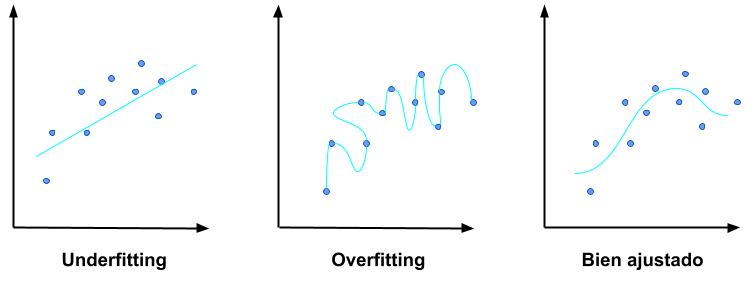
\includegraphics[width=0.8\textwidth]{img/overfitting.png}
    \caption{Ejemplo de sobreajuste, subajuste y buen ajuste.}
    \label{fig:overfitting}
\end{figure}

Por último, la gráfica de más a la derecha presenta un ajuste idóneo para este conjunto de datos, ya que se puede observar como se ajusta a todos los puntos pero sin capturar ruido. Para llegar a este tipo de ajuste y evitar los dos primeros casos, vamos a explorar diferentes métodos para mitigar el sobreajuste, como la regularización $l1$ y $l2$, las capas dropout o la parada temprana.

\subsection{Regularización l1 y l2} \label{sec:regularizacion}

La regularización ayuda a evitar el sobreajuste, lo cual ocurre cuando un modelo es demasiado complejo y comienza a captar el ruido o los patrones irrelevantes en los datos de entrenamiento. En lugar de eso, la regularización favorece la creación de modelos más simples que pueden identificar los patrones importantes y generalizar mejor a datos nuevos. Esta técnica es especialmente útil cuando se tiene una cantidad limitada de datos, conjuntos de datos con muchas características o modelos con muchos parámetros \citep{pajares2021aprendizaje}.

Para implementarla, se añade un término de regularización a la función de pérdida durante el entrenamiento. Este término penaliza ciertos parámetros del modelo, ajustando el total de la pérdida. La intensidad de la regularización se controla mediante un parámetro que determina el equilibrio entre ajustar los datos y reducir el impacto de coeficientes muy grandes \citep{geron2022hands}.

\begin{equation}
loss_{regul}(\theta) = loss(\theta) + \beta \cdot f(\theta) 
\end{equation}

Aquí, \( loss_{regul}(\theta) \) es la función de pérdida final despues de aplicarle una regularización. \( loss(\theta) \) es la función de pérdida original que mide el ajuste del modelo a los datos, y \( \theta \) representa los parámetros del modelo (pesos y sesgos). El parámetro \(\beta\) controla la intensidad de la regularización, equilibrando entre ajustar el modelo a los datos y mantener los valores de los parámetros bajo control. Por último, el término de regularización \( f(\theta) \) penaliza los parámetros del modelo, siendo comúnmente la regularización $l2$ o la $l1$. 
 

La \textbf{regularización \(l2\)} (o regresión Ridge) añade una penalización proporcional a la suma de los pesos al cuadrado. La función de pérdida regularizada \(l2\) se define como:

\begin{equation}
\text{Loss} = \text{Original Loss} + \lambda \sum_{i} w_i^2
\end{equation}

donde \(\lambda\) es el parámetro de regularización que controla la importancia de la penalización y $w_i$ los pesos \citep{geron2022hands}. Este método tiende a producir soluciones más estables y reduce la complejidad de los modelos, tendiendo los coeficientes hacia valores más pequeños.


La \textbf{regularización \(l1\)} (o regresión Lasso) añade una penalización proporcional a la suma del valor absoluto de los pesos:
\begin{equation}
\text{Loss} = \text{Original Loss} + \lambda \sum_{i} |w_i|
\end{equation}
Esta técnica puede generar un modelo más sencillo, donde algunos coeficientes se anulan, seleccionando las características más importantes de los datos. Sin embargo, produce soluciones menos estables que aplicando $l2$ \citep{geron2022hands}. 


\subsection{Dropout} \label{sec:dropout}

Otro método para evitar el sobreajuste de nuestro modelo es el Dropout, que fue propuesto por Hinton et al. \citep{hinton2012improving} como una forma de regularización para capas de redes neuronales completamente conectadas. El dropout consiste en que cada elemento de la salida de una capa se mantiene en cada iteración con una probabilidad \(p\) (``tasa de dropout''), de lo contrario se establece en 0, con una probabilidad \((1 - p)\). Según \citep{geron2022hands}, este valor de $p$ suele variar entre 0.1 y 0.5, siendo este último uno de los más típicos \citep{srivastava2013improving}, aunque la red neuronal que se esté utilizando influye en el valor óptimo \citep{geron2022hands}. La elección de este parámetro es muy importnate, ya que si tomamos un valor muy alto, puede llevarnos a underfitting.
    
\begin{figure}[H]
    \centering
    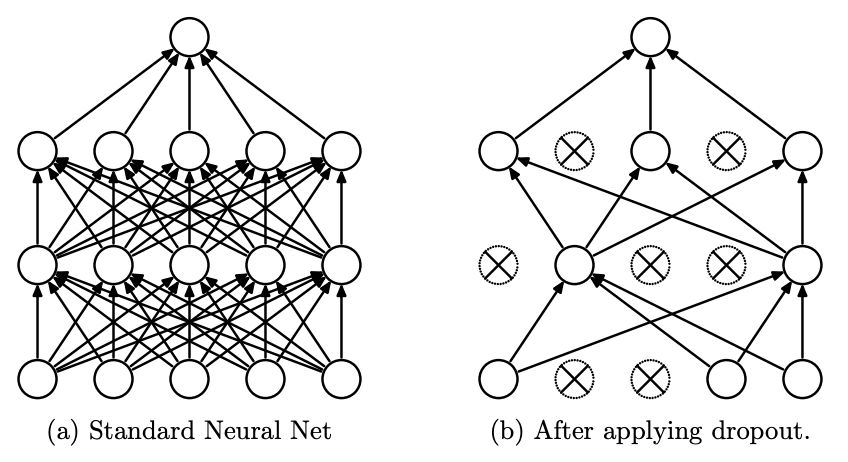
\includegraphics[width=0.6\textwidth]{img/dropout.png}
    \captionof{figure}{Esquema de la técnica dropout. Fuente \citep{srivastava2014dropout}}
    \label{fig:dropout}
\end{figure}
    
Al eliminar una neurona, esta se elimina de la red con todas sus conexiones entrantes y salientes (ver Figura \ref{fig:dropout}). La principal ventaja de esto es que la red no depende excesivamente de ninguna neurona, mejorando de esta forma la generalización del modelo. La eliminación se aplica de manera independiente a cada capa oculta y a cada iteración del entrenamiento. 


Por lo tanto, aplicar dropout a una red neuronal equivale a seleccionar una submuestra ``reducida'' de la red original. Como cada neurona puede estar activa o inactiva, hay un total de $2^n$ redes posibles, donde $n$ es el número de neuronas que se pueden desactivar \citep{srivastava2013improving}. Puede interpretarse como entrenar una gran colección de redes neuronales diferentes y usar sus promedios para hacer predicciones.


Experimentos como los que se harán en el Capítulo \ref{Capitulo_3} muestran como el Dropout mejora la capacidad de generalización de la red, proporcionando un mejor rendimiento del modelo.


El uso del dropout en una red neuronal se implementa fácilmente en frameworks como Keras. Por ejemplo:

\lstset{language=Python}
\begin{lstlisting}
from tensorflow.keras.layers import Dropout

model = Sequential([
    Dense(128, activation='relu'),
    Dropout(0.5),
    Dense(10, activation='softmax') ])
\end{lstlisting}

En este código, se aplica dropout con una tasa del 50\% después de una capa densa con 128 unidades.



\subsection{Parada temprana}

Además de las técnicas de regularización $l1$ y $l2$ y el uso de dropout para prevenir el sobreajuste en redes neuronales, otra estrategia ampliamente utilizada es la parada temprana o \textit{Early Stopping}.

\begin{minipage}{0.35\textwidth}
\centering
    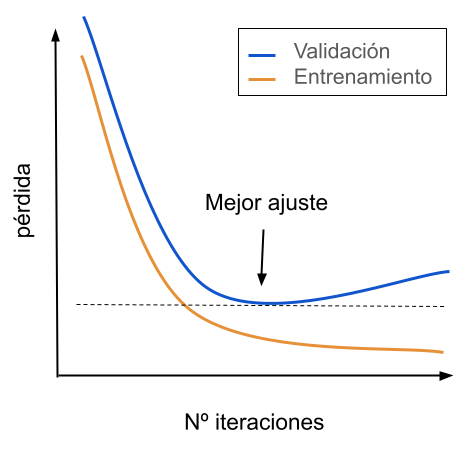
\includegraphics[width=0.8\textwidth]{img/earlyStopping.png}
    \captionof{figure}{Curvas de error de entrenamiento y validación con Early Stopping.}
    \label{fig:early_stopping}
\end{minipage}
\begin{minipage}{0.6\textwidth}
     El Early Stopping consiste en que el modelo deja de entrenar cuando el error en el conjunto de validación alcanza un mínimo y comienza a aumentar nuevamente. Esto se observa durante el proceso de entrenamiento, cuando el error de entrenamiento continúa disminuyendo mientras que el error de validación inicialmente disminuye, pero eventualmente comienza a incrementarse debido al sobreajuste \citep{geron2022hands}. La Figura \ref{fig:early_stopping} ilustra este comportamiento, donde la precisión del modelo en el conjunto de validación deja de mejorar después de cierto punto y comienza a empeorar.
     
\bigskip

Formalmente, si denotamos el error en el conjunto de entrenamiento después de la \( t \)-ésima época como \( E_{\text{tr}}(t) \) y el error en el conjunto de validación como \( E_{\text{val}}(t) \), Early Stopping interrumpe el entrenamiento cuando \( E_{\text{val}}(t) \) deja de mejorar durante un número definido de épocas consecutivas. 
\end{minipage}


Esta técnica no solo ayuda a prevenir el sobreajuste sino que también optimiza el uso de recursos al detener el entrenamiento cuando ya no se obtienen mejoras en el desempeño del modelo \citep{tian2022comprehensive}.

Para implementarlo en la práctica, frameworks como Keras ofrecen callbacks que facilitan este proceso. A continuación se presenta un ejemplo de código que utiliza \lstinline|EarlyStopping| para detener el entrenamiento cuando no se observa ninguna mejora en el error de validación:


\lstset{language=Python}
\begin{lstlisting}
from tensorflow.keras.callbacks import EarlyStopping

early_stopping_cb = keras.callbacks.EarlyStopping(patience=10,
                                           restore_best_weights=True)
history = model.fit(X_train, y_train, epochs=100,
                    validation_data=(X_valid, y_valid),
                    callbacks=[early_stopping_cb])
\end{lstlisting}

En este ejemplo, EarlyStopping detiene el entrenamiento después de un número definido de épocas sin mejora (\lstinline|patience = 10|), restaurando los pesos que lograron el mejor desempeño \citep{geron2022hands}.

Así, \textit{Early Stopping} se complementa eficazmente con las técnicas de regularización $l1$, $l2$ y dropout, proporcionando una capa adicional de protección contra el sobreajuste y mejorando la robustez del modelo.

\bigskip


El sobreajuste es uno de los principales desafíos en el entrenamiento de modelos de aprendizaje automático, incluyendo las redes neuronales. Técnicas como la regularización \(l2\), el dropout y la parada temprana son estrategias efectivas para mitigar este problema. Es crucial seleccionar y combinar adecuadamente estas técnicas según las características del problema y los datos disponibles. A través de estos métodos, podemos mejorar la capacidad de generalización de nuestros modelos y lograr un rendimiento más robusto en datos no vistos \citep{geron2022hands, pajares2021aprendizaje}.












\section{Evaluación del modelo.} CYA HE ESTUDIADO SUPERVISADO, NO SUPERVISADO Y LOS MÉTODOS DE ML.


Una vez discutidos los fundamentos del aprendizaje supervisado y no supervisado, y explorado una variedad de algoritmos de machine learning, profundizaremos ahora en la evaluación de los diferenes modelos. Nos centraremos en los métodos supervisados, tanto en regresión como en clasificación, ya que la evaluación y selección de modelos en aprendizaje no supervisado suele ser un proceso más cualitativo \citep{muller2016introduction}. 


Para evaluar los modelos supervisados, primero se divide el conjunto de datos en un conjunto de entrenamiento y un conjunto de prueba utilizando la función \lstinline|train_test_split|, que divide los datos de manera aleatoria. Algunos modelo como la \acrshort{cnn} o los autoencoders también necesitan un conjunto de validación durante su entrenamiento para ir evaluando el rendimiento del modelo en cada iteración. Además, proporciona información muy valiosa para detectar si un modelo empieza a sobreaprender de los datos de entrenamiento. Los porcentajes de estos subconjuntos suelen encontrarse entre el 70 - 80 \%, 10 - 20 \% y 10 - 20 \% para entrenamiento, test y validación respectivamente. El conjunto de entrenamiento sirve para entrenar la red neuronal. Por otro lado, el conjunto de prueba sirve para medir definitivamente el rendimiento del modelo con nuevas muestras de datos que no han sido utilizadas durante del entrenamiento para evaluar el modelo \citep{muller2016introduction}.


El problema de esta técnica radica en que las distribuciones de los datos pueden no ser uniformes en los tres subconjuntos y que no sea una divisón muy óptima. Para evitar este inconveniente, se puede usar una técnica de evaluación del modelo más avanzada llamada \textbf{validación cruzada} (\textit{cross-validation}), donde los datos se dividen en varios subconjuntos, y el modelo se entrena y valida múltiples veces, garantizando una evaluación más robusta del rendimiento. La variante más comúnmente utilizada es la validación cruzada \textit{k-fold}. Aquí, el conjunto de datos se divide en $k$ partes aproximadamente iguales, llamadas pliegues. Cada uno de los $k$ pliegues se utiliza una vez como conjunto de prueba, mientras que los $k-1$ pliegues restantes se combinan para formar el conjunto de entrenamiento. Este proceso se repite $k$ veces, generando $k$ modelos y $k$ evaluaciones. La Figura~\ref{fig:kfold} ilustra este procedimiento \citep{muller2016introduction}.

\begin{figure}[h]
	\centering
    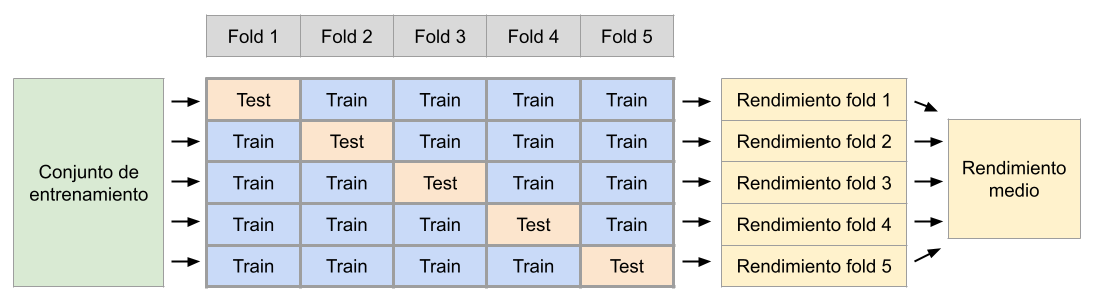
\includegraphics[width=0.6\textwidth]{img/kfold.png}
    \captionof{figure}{Validación cruzada k-fold.}
    \label{img: k-fold}
\end{figure}

Al final de la validación cruzada \textit{k-fold}, se recopilan $k$ valores de desempeño (por ejemplo, precisión en clasificación) que se pueden promediar para obtener una estimación más robusta del rendimiento del modelo. La validación cruzada no solo proporciona una evaluación más precisa del modelo, sino que también ayuda a detectar variaciones en el desempeño debido a diferentes particiones de datos, ofreciendo así una visión más completa de la capacidad del modelo para generalizar \citep{muller2016introduction}. Aunque la validación cruzada ofrece bastantes beneficios, su uso es menos frecuente en redes neuronales debido a los altos costos computacionales asociados \citep{geron2022hands}. En su defecto, es más frecuente usar \lstinline|train_test_split()|.



Una vez ya se ha entrenado el modelo, utilizamos el conjunto de prueba para medir el rendimiento del modelo. Para ello, se utilizan una serie de métricas que nos permiten entender el rendimiento y efectividad de un modelo. A continuación, se describen las principales métricas utilizadas, así como las representaciones gráficas asociadas.

\subsection{Matriz de Confusión}

La matriz de confusión es una herramienta que nos permite visualizar el rendimiento del modelo al mostrar los conteos de verdaderos positivos (TP), falsos positivos (FP), verdaderos negativos (TN) y falsos negativos (FN). Cada fila de la matriz representa las etiquetas reales mientras que cada columna representa las etiquetas predichas.

La matriz se define como:
\[
\begin{array}{c|cc}
 & \text{Predicción Positiva} & \text{Predicción Negativa} \\
\hline
\text{Real Positiva} & TP & FN \\
\text{Real Negativa} & FP & TN \\
\end{array}
\]

Para calcularla, utilizamos el conjunto de predicciones del modelo y las etiquetas reales. La matriz de confusión nos ofrece una visión clara de cómo se distribuyen los errores del modelo entre las diferentes clases.

\subsection{Métricas}

La matriz de confusión ofrece una gran cantidad de información, pero a veces te interesa una métrica más concreta para evaluar un modelo de clasificación, como la sensibilidad, la tasa de falsos negativos o su sensibilidad. A continuación vamos a definir y explicar las principales métricas a tener en cuenta según \citep{erickson2021magician} junto con su fórmula. 

La \textbf{sensibilidad} es la fracción de casos positivos que el modelo predice correctamente como positivos. También se conoce como recall o tasa de verdaderos positivos (TPR). Se calcula utilizando la fórmula:
\[
\text{Sensibilidad} = \frac{TP}{TP + FN}
\]

La \textbf{especificidad} es la fracción de casos negativos que el modelo predice correctamente como negativos. También se conoce como selectividad o tasa de verdaderos negativos (TNR). Se calcula utilizando la fórmula:
\[
\text{Especificidad} = \frac{TN}{TN + FP}
\]

La \textbf{tasa de falsos positivos} (FPR) es la fracción de casos negativos que el modelo predice incorrectamente como positivos. También se conoce como fall-out o probabilidad de alarma falsa. Se calcula utilizando la fórmula:
\[
\text{FPR} = \frac{FP}{TN + FP}
\]

La \textbf{tasa de falsos negativos} (FNR) es la fracción de casos positivos que el modelo predice incorrectamente como negativos. También se conoce como tasa de error tipo II o tasa de omisión. Se calcula utilizando la fórmula:
\[
\text{FNR} = \frac{FN}{TP + FN}
\]

El \textbf{valor predictivo positivo} (PPV) es la fracción de casos que el modelo predijo como positivos que realmente son positivos. También se conoce como precisión. Se calcula utilizando la fórmula:
\[
\text{PPV} = \frac{TP}{TP + FP}
\]

El \textbf{valor predictivo negativo} (NPV) es la fracción de casos que el modelo predijo como negativos que realmente son negativos. Se calcula utilizando la fórmula:
\[
\text{NPV} = \frac{TN}{TN + FN}
\]

El \textbf{accuracy} es la fracción de casos que el modelo predijo correctamente, ya sean positivos o negativos. Se calcula utilizando la fórmula:
\[
\text{Accuracy} = \frac{TP + TN}{TP + FN + TN + FP}
\]

Por último la \textbf{puntuación F1} es la media armónica del valor predictivo positivo y la sensibilidad. También se conoce como puntuación F, medida F o coeficiente de similitud de Dice. Se calcula utilizando la fórmula:
\[
\text{Puntuación F1} = \frac{2TP}{2TP + FP + FN}
\]



\subsection{Curva ROC y AUC}

\begin{minipage}{0.5\textwidth}
La curva ROC (Receiver Operating Characteristic) es otra herramienta utilizada en los modelos de clasificación \citep{geron2022hands}. Consiste en una representación gráfica que muestra la relación entre la tasa de verdaderos positivos (TPR) y la tasa de falsos positivos (FPR) para diferentes umbrales de clasificación. La linea discontinua de la figura \ref{img: roc} indica la curva ROC de un clasificador puramente aleatorio \citep{geron2022hands}. 

\bigskip

Otro término que está relacionado es el AUC (\textit{area under the curve}). El AUC es el área que se encuentra encerrada entre la curva ROC, la recta $y = 0$ y $x = 1$. Cuantifica la capacidad que tiene el modelo para distinguir entre las diferentes clases. Cuanto mayor valor, mejor rendimiento. En la Figura \ref{img: roc} se representa con rallas de intensidad baja. 
\end{minipage}
\begin{minipage}{0.05\textwidth}
\textbf{ }
\end{minipage}
\begin{minipage}{0.4\textwidth}
	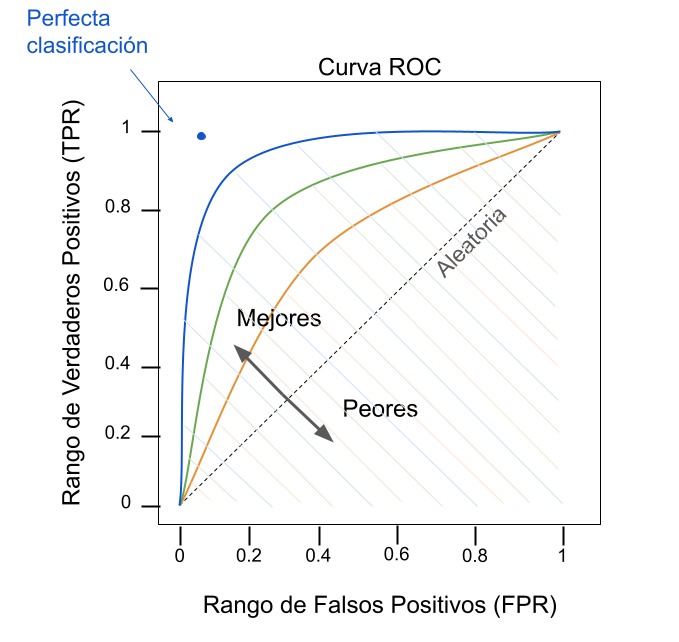
\includegraphics[width=1.15\textwidth]{img/roc.png}
	\captionof{figure}{Interpretación de la curva ROC con el área bajo la curva (AUC).}
	\label{img: roc}
\end{minipage}

La interpretación de estos términos consiste en que una curva ROC más cercana al vértice superior izquierdo, o un AUC cercano a 1, indica un mejor rendimiento del modelo \citep{geron2022hands}.

\subsection{Curva de Precisión-Recall}

\begin{minipage}{0.4\textwidth}
	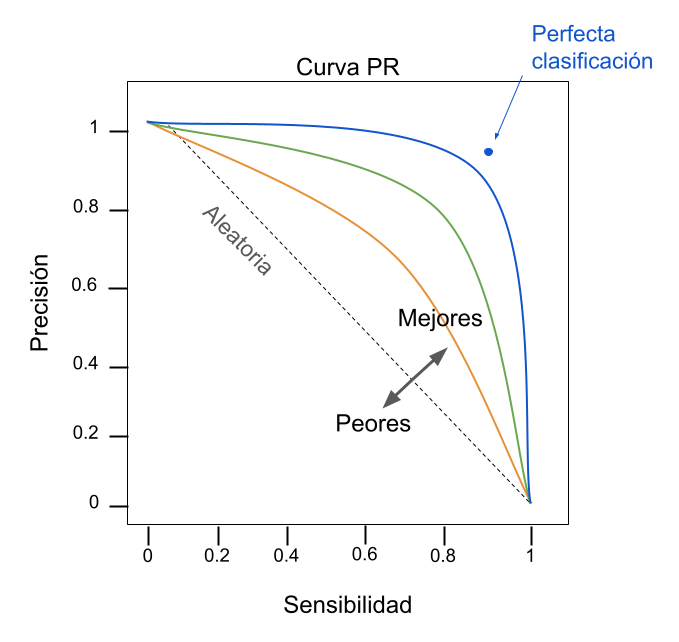
\includegraphics[width=1.15\textwidth]{img/pr.png}
	\captionof{figure}{Curva de Precisión-Recall.}
	\label{img: pr}
\end{minipage}
\begin{minipage}{0.05\textwidth}
\textbf{ }
\end{minipage}
\begin{minipage}{0.5\textwidth}
Por último, se estudiará la curva de Precisión-Recall (PR). Esta curva muestra la precisión frente a la sensibilidad para diferentes umbrales de decisión. Se identifica a partir de qué valor de sensibilidad comienza una disminución en la precisión, y viceversa. Idealmente, se busca una curva que se acerque lo más posible a la esquina superior derecha del gráfico, lo que representaría una combinación óptima de alta precisión y alto recall.

\bigskip

Esta curva es especialmente útil para ajustar un umbral de decisión que permita obtener una precisión tan alta como se desee, pero a costa de la sensibilidad. Por ejemplo, si se desea una precisión del 90\%, se puede aumentar el umbral has-
\end{minipage}

ta alcanzar este valor de precisión, aunque esto reducirá la sensibilidad. Este proceso se denomina trade-off entre precisión y sensibilidad.

Para calcular este umbral, se utilizan las puntuaciones de decisión obtenidas del clasificador. Primero, se obtienen estas puntuaciones usando la función \lstinline|decision_function()| del clasificador. Luego, se emplea la función \lstinline|precision_recall_curve()| de Scikit-Learn para calcular la precisión y la sensibilidad para todos los umbrales posibles. Finalmente, se selecciona el umbral que proporciona la precisión deseada. La Figura \ref{img: pr_vs_threshold} ilustra cómo se comportan la precisión y la sensibilidad en función del umbral \citep{geron2022hands}.

\begin{figure}[h]
	\centering
    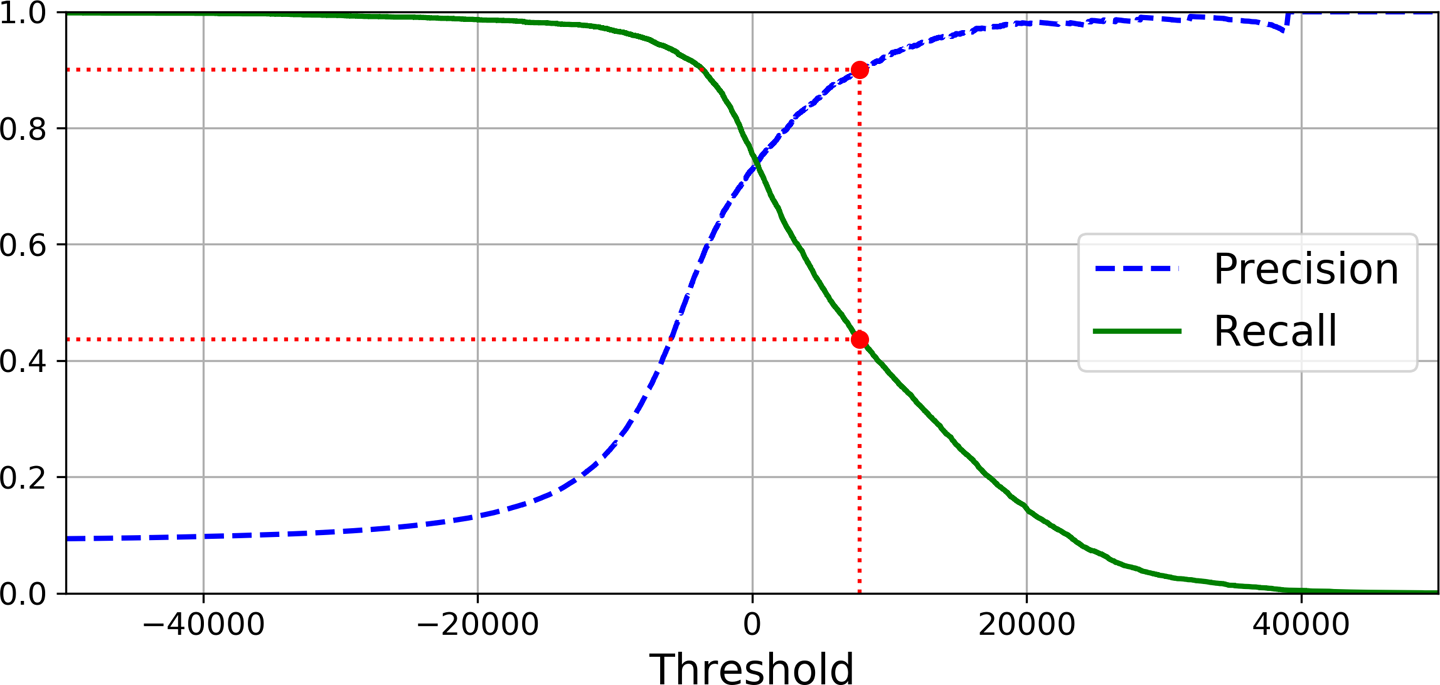
\includegraphics[width=0.6\textwidth]{img/precision_recall_vs_threshold.png}
    \captionof{figure}{Precisión y Sensibilidad vs Umbral de decisión. Fuente \citep{geron2022hands}}
    \label{img: pr_vs_threshold}
\end{figure}











\section{Arquitecturas relevantes} \label{Subsec: 3_2}
Mini tabla resumen en Deep Cybersecurity: A Comprehensive Overview from Neural Network and Deep Learning Perspective y miniresumen de todos los tipos en review Deep Cybersecurity: A Comprehensive Overview from Neural Networkand Deep Learning Perspective y review

\subsection{Autoencoder}

Los autoencoders son una clase de redes neuronales artificiales utilizadas en aprendizaje no supervisado para aprender representaciones eficientes de los datos. Su funcionamiento consiste en codificar la entrada en una representación comprimida y significativa, y luego decodificarla de manera que la reconstrucción sea lo más similar posible a la entrada original \citep{lopes2022effective}. La arquitectura básica de un autoencoder consta de tres partes: el encoder, el cuello de bottela y el decoder (Figura \ref{fig:AE_architecture}). 


\begin{figure}[h]
    \centering
    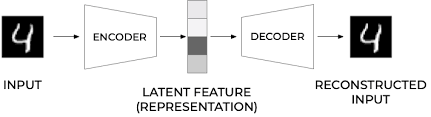
\includegraphics[width=0.6\textwidth]{img/AE4.png}
    \caption{Arquitectura de un autoencoder. Fuente:\citep{autoencoderImage}.}
    \label{fig:AE_architecture}
\end{figure}




el autoencoder ilustrado en la figura \ref{fig:ae_structure} puede modelarse mediante la ecuación (\ref{eq:ae_model}).

\begin{equation}
\begin{cases}
z = f(x; w_e, b_e) \\
r = g(z; w_d, b_d)
\end{cases}
\label{eq:ae_model}
\end{equation}

donde $f(\cdot)$ y $g(\cdot)$ son funciones del codificador y del decodificador que generalmente se implementan mediante redes neuronales. Los parámetros $w_e$ y $b_e$ son del codificador, y $w_d$ y $b_d$ son del decodificador. Si $f(\cdot)$ y $g(\cdot)$ son redes neuronales, entonces $w_i$ y $b_i$ son las matrices de pesos y los vectores de sesgo con respecto a la red neuronal del codificador y la red neuronal del decodificador ($ \forall i \in  {e, d}$). El codificador (encoder) mapea el conjunto de datos $x$  al espacio de características $z$ que normalmente suene tener una menor dimensión. Por otra parte, el decodificador (decoder) reconstruye los datos iniciales $x$ a través de la representación comprimida oculta $z$ \citep{zhai2018autoencoder}. Durante el entrenamiento, los parámetros del autoencoder se optimizan para minimizar la diferencia entre la entrada y la salida reconstruida, utilizando una función de pérdida que mide esta discrepancia, como por ejemplo la \lstinline|binary_crossentropy| o el \lstinline|mse|. La expresión matemática puede expresarse como:
\begin{equation}
\arg \min_{A, B} \mathbb{E}[\Delta(x, B \circ A(x))]
\end{equation}
donde $\mathbb{E}$ es la esperanza sobre la distribución de $x$, y $\Delta$ es la función de pérdida de reconstrucción, que mide la distancia entre la salida del decodificador y la entrada \citep{bank2023autoencoders}. Esto concluye el proceso de entrenamiento de un autoencoder.


Las ecuaciones para obtener la salida de un autoencoder serían:
\[
\left\{
\begin{aligned}
z^{(1)} &= W^{(1)} \cdot x + b^{(1)} \\
a^{(2)} &= f(z^{(1)})  \\
z^{(2)} &= W^{(2)} \cdot a^{(2)} + b^{(2)}  \\
y &= z^{(2)} 
\end{aligned}
\right.
\]

donde  $x$ es el input, \( b^{(1)} \) y  \( b^{(2)} \) son los sesgos,  \( W^{(1)} \) y  \( W^{(2)} \) son los pesos, \( z^{(1)} \) es la salida lineal de la primera capa, \( a^{(2)} \) es la activación de la segunda capa, \( z^{(2)} \) es la salida lineal de la segunda capa e \( y \) es la salida final del modelo \citep{martinez2017analisis}.


Tradicionalmente, los autoencoders se empleaban principalmente para reducir la dimensionalidad o para extraer características. No obstante, con el auge de diversos modelos de aprendizaje profundo, especialmente los modelos de redes generativas adversarias, los autoencoders han cobrado relevancia en la modelización generativa. Esto ha llevado a numerosos investigadores a proponer una variedad de modelos extendidos de autoencoders, como las convolutional autoencoders (que veremos en más profundidad en la sección \ref{sec:2.CNN}) o los recurrentes \citep{zhai2018autoencoder}. 

Las principales capas que se utilizan en esta red neuronal son las capas densas y las de aplanamiento, aunque también se pueden utilizar capas convolucionales traspuestas y capas unpooling (sección \ref{sec:2.CNN}) para autocodificadores convolucionales\footnote{Autocodificador para imágenes de gran tamaño} o LSTM en el caso de autocodificadores recurrentes\footnote{Autocodificador específico para series temporales o secuencias.}\citep{geron2022hands}. 




\subsection{Deep Belief Networks}
\subsubsection{Red Neuronal Profunda}
\subsection{Red Neuronal Convolucional} \label{sec:2.CNN}


Las redes neuronales convolucionales son una de las métodos de machine learning más importantes y utilizados en el campo de la ciberseguridad. Estas redes neuronales están diseñadas para procesar entradas almacenadas en matrices, como las imágenes.  Son una parte de las redes profundas que procesa y analiza entradas de imágenes visuales, y están compuestas por neuronas con pesos y sesgos que aprenden a lo largo de su entrenamiento \citep{podder2021artificial}. La arquitectura de una CNN (Figura \ref{fig:cnn_architecture}) consta de tres tipos de capas: capas de convolución, capas de pooling y la capa de clasificación. 
 

\begin{figure}[h]
    \centering
    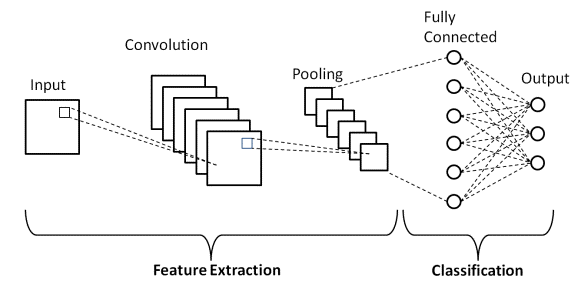
\includegraphics[width=0.6\textwidth]{img/convlayers.png}
    \caption{Arquitectura de una CNN con capas de convolución, pooling y clasificación. Fuente:\citep{phung2018deep}.}
    \label{fig:cnn_architecture}
\end{figure}

\subsubsection*{Capa convolucional}

La capa convolucional es la capa más importante de una \acrshort{cnn}. En ella se extraen las características más significativas de la imagen de entrada, como los bordes, el color o la forma. Para ello se aplica una convolución a la imagen con un filtro. Esta operación matemática se representa como \( \int (x \star w)(t) \) donde $x$ representa la entrada y $w$ el núcleo de convolución \citep{pajares2021aprendizaje}.


En una CNN, la entrada de la convolución es una matriz multidimensional junto con una matriz de parámetros $w$ que se ajusta durante el aprendizaje (llamada núcleo o filtro). Cada píxel de la capa de convolución tiene una neurona, que se conecta con la capa anterior aplicando la convolución con las neuronas de su campo receptivo\footnote{Región de entrada que contribuye a la salida generada por el filtro} \cite{geron2022hands}. Esta convolución se realiza con un solapamiento total del filtro, lo que resulta en una imagen de menor dimensión (Figura \ref{fig:convolucion}). Si se desea mantener la misma dimensión, se puede aplicar zero-padding, que consiste en rellenar con ceros la matriz para obtener las dimensiones deseadas (Figura \ref{fig:convolucionPadding}). En la figura \ref{fig:convolu2} se muestran sendos campos receptivos de la imagen \( I \) que contribuyen a las salidas \( P \) y \( Q \) generadas por el filtro \( K \). La matriz de respuesta al aplicarle el kernel se llama mapa de características ($O$).


\begin{figure}[h] 
     \centering
     \begin{subfigure}[b]{0.45\textwidth}
         \centering
         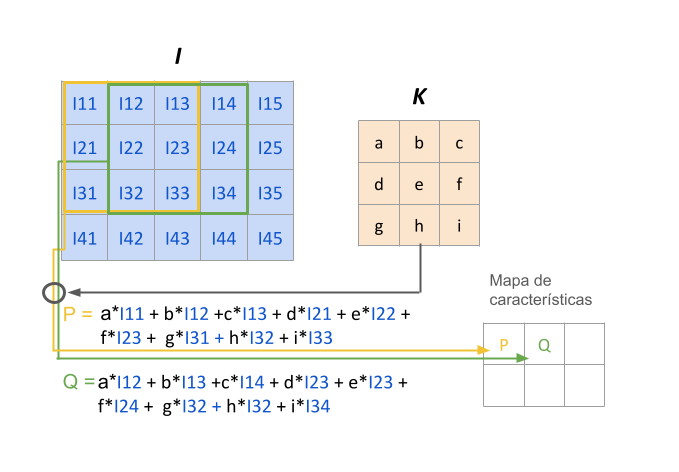
\includegraphics[width=\textwidth]{img/convolucion.png}
         \caption{Convolución reduciendo tamaño.}
         \label{fig:convolucion}
     \end{subfigure}
     \hfill
     \begin{subfigure}[b]{0.45\textwidth}
         \centering
         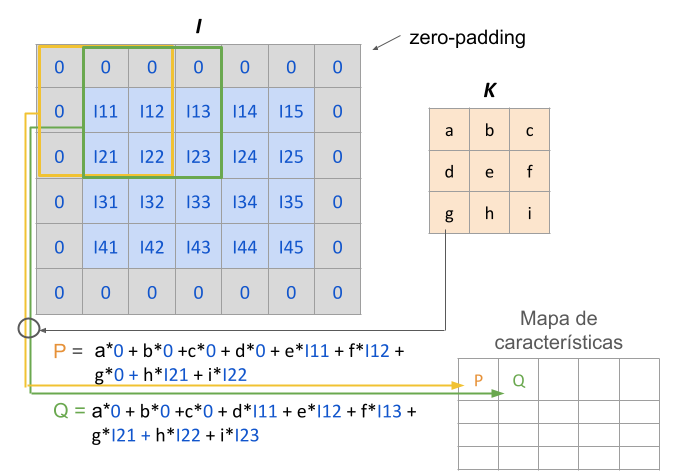
\includegraphics[width=1\textwidth]{img/convolucionPadding.png}
         \caption{Convolución con zero-padding.}
         \label{fig:convolucionPadding}
     \end{subfigure}
     \caption{Convolución en 2D.}
     \label{fig:convolu2}
\end{figure} 

Se observa que el filtro se desplaza por la matriz \textit{I} con paso unitario en vertical y horizontal. Este parámetro se llama stride y su valor depende de el objetivo que se quiera lograr con esta capa convolucional.

\begin{figure}[h]
    \centering
    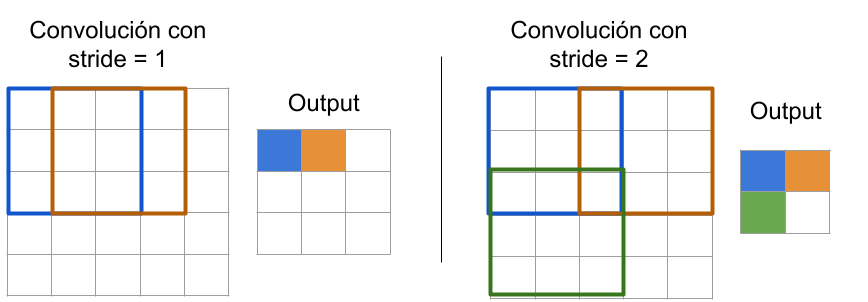
\includegraphics[width=0.6\textwidth]{img/stride.png}
    \caption{Campos receptivos en una convolución. Adaptación de imagen de \citep{yepez2020stride}}
    \label{fig:receptive_field}
\end{figure}

Una longitud de paso de 1 se utiliza normalmente para extraer el máximo número de características, ya que proporciona el máximo solapamiento entre el núcleo y la entrada. Por otro lado, cuando la longitud de paso es mayor que 1, los campos receptivos se solapan menos y producen una salida más pequeña. Si la longitud de paso fuera 3, habría problemas con el espaciado, ya que el campo receptivo no encajaría alrededor de la entrada como un número entero \citep{yepez2020stride}.



Por simplicidad, se ha usado siempre un único kernel, pero se puede generalizar a varios filtros, creando un mapa de características por cada uno. En cada uno de estos mapas hay una neurona por pixel y todas ellas comparten los mismos parámetros, lo que reduce considerablemente el número de parámetros del modelo. El campo receptivo de una neurona ahora se extiende por los mapas de características de todas las capas anteriores \citep{geron2022hands}.



Toda la información anterior se resume en la siguiente ecuación \citep{pajares2021aprendizaje}:

\begin{equation}
z_{i,j,k} = b_k + \sum_{u=0}^{f_h-1} \sum_{v=0}^{f_w-1} \sum_{k'=0}^{f_n'-1} x_{i',j',k'} \cdot w_{u,v,k',k} \hspace{5mm} \textup{con }
\left\{
\begin{array}{l}
i' = i \cdot s_h + u \\
j' = j \cdot s_w + v
\end{array}
\right.
\end{equation} \label{eq:conv}

donde:
\begin{itemize}
    \item \( z_{i,j,k} \) es la salida de la neurona ubicada en la fila \(i\), columna \(j\) en el mapa de características \(k\) de la capa convolucional (capa \(l\)).
    \item \( s_h \) y \( s_w \) son los pasos de avance vertical y horizontal.
    \item \( f_h \) y \( f_w \) son la altura y la anchura del campo receptivo y \( f_{n'} \) es el número de mapas de características de la capa anterior (capa \(l-1\)).
    \item \( x_{i',j',k'} \) es la salida de la neurona situada en la fila \(i'\), columna \(j'\), mapa de características \(k'\).
    \item \( b_k \) es el sesgo para el mapa de características \(k\) (en la capa \(l\)).
    \item \( w_{u,v,k',k} \) es el peso de conexión entre cualquier neurona del mapa de características \(k\) de la capa \(l\) y su entrada situada en la fila \(u\), columna \(v\) (relativa al campo receptivo de la neurona) y el mapa de características \(k'\).
\end{itemize}





\subsubsection*{Capa de pooling}

El siguiente tipo de capa de las \acrshort{cnn} son las pooling, cuyo objetivo es reducir la imagen de entrada para disminuir la carga computacional, el uso de memoria y el número de parámetros, limitando así el riesgo de sobreajuste y proporcionando robustez contra el ruido y las distorsiones. Esta capa se suele colocar entre las capas de convolución, permitiendo reducir el tamaño de las imágenes mientras se preservan las características más importantes \citep{podder2021artificial}. Al igual que en las capas convolucionales, sus neuronas están conectadas a un pequeño grupo de neuronas de la capa anterior a las que se le aplica una función de agregación\footnote{Las funciones de agregación devuelven un valor único de un conjunto de registros.}. Las tres funciones más comunes son el promedio, la suma y el máximo. La Figura \ref{fig:maxpooling} muestra una capa de max pooling, que es el tipo más común \citep{geron2022hands}. 



\begin{figure}[h!]
\centering
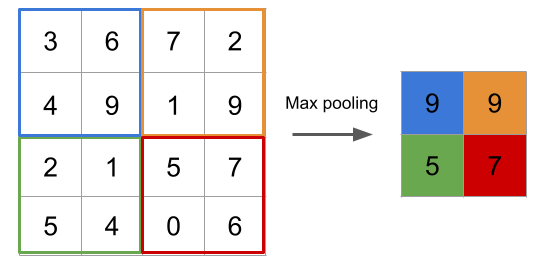
\includegraphics[width=0.4\textwidth]{img/maxpooling.png}
\caption{Capa de max pooling con un kernel de \( 2 \times 2 \), stride 2 y sin padding.}
\label{fig:maxpooling}
\end{figure}

Además de reducir el número de operaciones, el número de parámetros y ayudar con el overfitting, una capa de max pooling introduce cierto nivel de invarianza a pequeñas translaciones, ya que si un pixel se traslada hacia la derecha, la salida también debería trasladarse un pixel hacia la derecha, como se ilustra en la Figura \ref{fig:translacionPooling}. Esto significa que pequeñas variaciones en la posición de las características dentro de la imagen no afectan significativamente la salida.


\begin{figure}[h!]
\centering
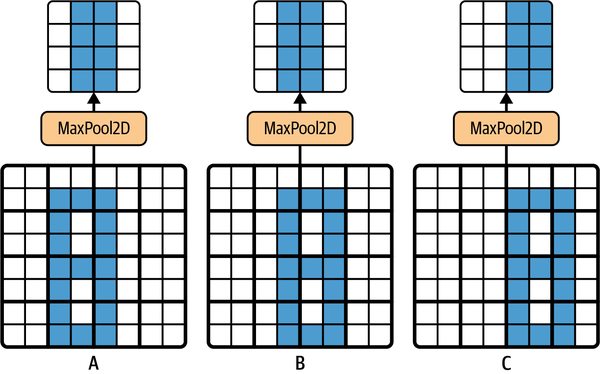
\includegraphics[width=0.4\textwidth]{img/translacionPooling.png}
\caption{Invarianza a translaciones pequeñas mediante una capa de max pooling. Fuente \citep{geron2022hands}}
\label{fig:translacionPooling}
\end{figure}

Una capa típica de convolución se compone de tres etapas. En la primera etapa, se realizan múltiples convoluciones para producir un conjunto de activaciones lineales. En la segunda etapa, cada activación lineal se procesa a través de una función de activación no lineal, como la función de activación rectificada lineal (ReLU). Esta etapa a menudo se denomina etapa de detección. En la tercera etapa, se aplica una función de pooling para modificar la salida de la capa. Este tipo de capa de convolución compuesta será de utilidad en los experimentos realizados en capítulos posteriores, como por ejemplo en la creación de una M-CNN para el problema de clasificación de malware del Capítulo \ref{Capitulo_3} \citep{pajares2021aprendizaje}.


\subsubsection*{Capa de Unpooling}

En la figura \ref{fig:maxpooling} se presenta un ejemplo gráfico relacionado con la operación de max pooling. Durante este proceso, es posible mantener un mapa de localizaciones, que señala la posición de origen del valor máximo que ha generado la capa. Este mapa permite ejecutar la operación inversa conocida como reconstrucción (Unpooling), colocando los valores obtenidos en las posiciones indicadas por el mapa de localizaciones. Una vez completada la reconstrucción, se puede realizar una interpolación lineal usando el método del vecino más próximo para obtener el mapa de características reconstruido \citep{pajares2021aprendizaje}. Este tipo de capa hace el proceso inverso de la capa de pooling. En vez de reducir la dimensión de entrada, la aumenta utilizando o bien interpolación lineal o bilineal o bien rellenando con ceros el resto de casillas \citep{pajares2021aprendizaje}. La operación de Unpooling se suele emplear junto con la operación de convolución transpuesta, como se describe más adelante, y se utiliza, por ejemplo, en el modelo de autoencoder utilizado en la sección \ref{sec: 3.AE}, en un autoencoder convolucional.

En Keras, esta capa se denomina \lstinline|UpSampling2D|.


\subsubsection*{Convolución Transpuesta}

La necesidad de realizar convoluciones transpuestas surge generalmente de la necesidad de aplicar una transformación en la dirección inversa a una convolución directa o normal, como la proyección de mapas de características a un espacio de mayor dimensión. Aunque a veces se denomina deconvolución, esta es en realidad una operación distinta. En las redes neuronales convolucionales (CNN), esta operación es más compleja que en las redes totalmente conectadas, donde solo se requiere el uso de una matriz de pesos transpuesta \citep{pajares2021aprendizaje}.

Considere la convolución mostrada en la figura \ref{fig:convolucion}. Sean $I$ y $O$ la entrada y la salida respectivamente expandidas en forma vectorial de izquierda a derecha y de arriba a abajo. Entonces la operación de convolución \ref{eq:conv} puede expresarse ahora como:

\begin{figure}[h!]
    \centering
    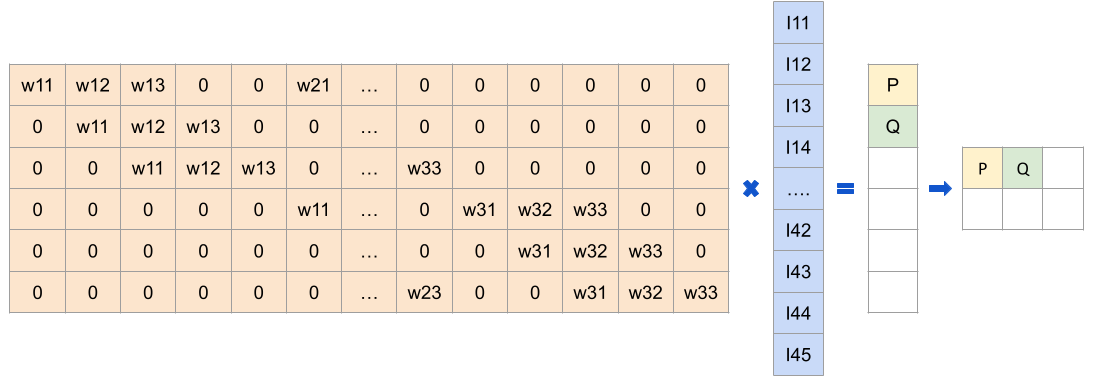
\includegraphics[width=0.8\textwidth]{img/conv2.png}
    \caption{Convolución y representación matricial.  $C \cdot I = O$}
    \label{fig:conv2}
\end{figure}

\begin{minipage}{0.5\textwidth}
La convolución puede ser expresada como una matriz dispersa \(C\), caracterizada por la presencia de múltiples ceros, donde los elementos no nulos corresponden a los elementos $w_{ij}$ del núcleo \(K\). Aquí, \(i\) y \(j\) denotan la fila y la columna, respectivamente. Esta operación lineal transforma la matriz de entrada en un vector de 20 dimensiones y produce un vector de 6 dimensiones, el cual se reestructura en una matriz de salida de \(2 \times 3\). Usando esta formulación, el paso hacia atrás se obtiene mediante la transposición de \(C\) \citep{pajares2021aprendizaje}.


\bigskip

Con la operación mencionada, se tiene un vector de 6 dimensiones como entrada y se obtiene un vector de 20 dimensiones como salida. En ambos casos, los valores $w_{ij}$ del núcleo definen las matrices \(C\) y \(C^t\) utilizadas en la propagación hacia delante y hacia atrás. Si se realiza la multipli-
\end{minipage}
\begin{minipage}{0.05\textwidth}
	\textbf{ }	
\end{minipage}
\begin{minipage}{0.45\textwidth}
	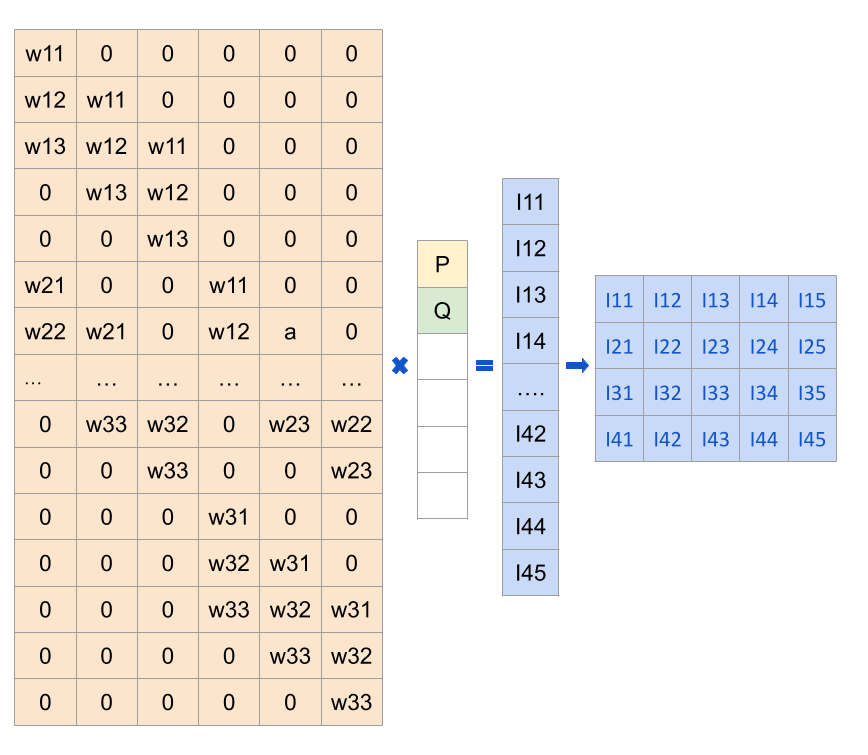
\includegraphics[width=1.1\textwidth]{img/convT.png}
    \captionof{figure}{Convolución traspuesta. $C^t \cdot O = I$.}
    \label{fig:convT}
\end{minipage}
cación matricial \(C^t \cdot O\), cuyas dimensiones son \(20x6\) y \(6x1\), se obtiene la matriz esperada $I$ de dimensión \(20x1\), que finalmente habrá que redimensionar \citep{pajares2021aprendizaje}.

Al igual que en las capas convolucionales originales, también puede añadirse zero-padding a la matriz y con desplazamientos (strides) superiores a la unidad \citep{pajares2021aprendizaje}.

Estas dos últimas capas son especialmente utilizadas en los autoencoderes convolucionales, donde hay que construir y reconstruir una versión reducida de los datos de entrada.

\subsubsection*{Capas Totalmente Conectadas (Fully Connected)}

Por último están las capas totalmente conectadas (\textit{fully connected}), que realizan la clasificación sobre la salida generada por las capas de convolución y pooling. Como el input de una capa densa debe ser un vector, primero se debe aplanar la salida de la última capa para poder utilizar después esta capa. Cada una de sus neuronas está conectada a todas las de la capa anterior, estableciendo una red densa de conexiones. Este tipo de neuronas suele ir seguido de una capa Dropout para mejorar la generalización del modelo. Este diseño permite a las CNN manejar datos complejos y variados, aprovechando la jerarquía de características aprendidas durante el entrenamiento. Este tipo de capa suele ir seguido de una capa de Dropout que mejora la capacidad de generalización del modelo al prevenir el sobreajuste, un problema común en el ámbito del aprendizaje profundo \citep{hossain2019classification}.



\subsection{Red Neuronal Recurrente}
\subsubsection{Restricted Boltzmann Machine}









\section{Bibliotecas utilizadas en Python} \label{Subsec: 3_3}

Para nuestros experimentos, utilizaremos Python debido a su popularidad y versatilidad en el ámbito del aprendizaje automático y la inteligencia artificial. Python ofrece una amplia gama de bibliotecas especializadas que facilitan la creación, entrenamiento y evaluación de modelos, así como el análisis y visualización de datos. A continuación, se describen las principales bibliotecas y frameworks que emplearemos en este trabajo, destacando sus características y ventajas.


\subsection{Principales frameworks. Keras}

Como las técnicas de aprendizaje profundo han ido ganando popularidad, muchas organizaciones académicas e industriales se han centrado en desarrollar marcos para facilitar la experimentación con redes neuronales profundas. En esta sección, ofrecemos una visión general de los marcos de trabajo más importantes que se pueden usar en Python, concluyendo con nuestra elección.


\textbf{TensorFlow} \citep{tensorflow} es una biblioteca de código abierto desarrollada por el equipo de Google Brain para la computación numérica y el aprendizaje automático a gran escala. Diseñada para ser altamente flexible, TensorFlow soporta computación distribuida y permite la optimización de gráficos computacionales, lo que mejora significativamente la velocidad y el uso de memoria de las operaciones. En su núcleo, TensorFlow es similar a NumPy pero con soporte para GPU, lo que acelera considerablemente los cálculos. Además, incluye herramientas avanzadas como TensorBoard para la visualización de modelos y TensorFlow Extended para la producción de modelos de aprendizaje automático. Gracias a estas capacidades, TensorFlow se ha convertido en una herramienta esencial en la industria y la investigación, siendo utilizada en aplicaciones que van desde la clasificación de imágenes y el procesamiento de lenguaje natural hasta los sistemas de recomendación y la previsión de series temporales.


\textbf{Keras} \citep{keras} es una API de alto nivel para redes neuronales que ahora es parte integral de TensorFlow. Fue desarrollada por François Chollet y ganó popularidad rápidamente gracias a su simplicidad y diseño elegante. Inicialmente, Keras soportaba múltiples backends, pero desde la versión 2.4, funciona exclusivamente con TensorFlow \citep{muller2016introduction}. Keras permite a los usuarios construir, entrenar y evaluar modelos de aprendizaje profundo de manera rápida y eficiente. Su facilidad de uso y extensa documentación la convierten en una herramienta valiosa tanto para la investigación como para la implementación de aplicaciones de inteligencia artificial.



\textbf{PyTorch} \citep{pytorch}, desarrollado por el equipo de investigación de IA de Facebook, es una biblioteca de aprendizaje profundo que destaca por su enfoque en la computación dinámica, lo que permite una mayor flexibilidad en la creación de modelos complejos. A diferencia de TensorFlow, que utiliza gráficos computacionales estáticos, PyTorch permite que la topología de la red neuronal cambie durante la ejecución del programa \citep{mahmoud2019dlbench}. Esto, junto con su capacidad de auto-diferenciación en modo inverso\footnote{Técnica en la que PyTorch calcula automáticamente las derivadas de las funciones de pérdida con respecto a los parámetros del modelo.}, hace que PyTorch sea popular entre los investigadores y desarrolladores. Su facilidad de uso y robusta comunidad de apoyo han llevado a su adopción por parte de importantes organizaciones como Facebook, Twitter y NVIDIA.



Para escoger con cuál de estas librerías se realizará la parte práctica de este trabajo, vamos a utilizar, además de las características previamente vistas, los resultados de \citep{mahmoud2019dlbench}. En él se hace un estudio de eficiencia, convergencia, tiempo de entrenamiento y uso de memoria de los diferentes frameworks con varios datasets. Entre sus resultados podemos observar como Keras destaca por encima de las demás en el entorno de la CPU. No solo logra el mejor accuracy en los tres datasets (MNIST, CIFAR-10, CIFAR-100), sino que además también tiene los tiempos de ejecución más bajos y una de las mejores tasas de convergencia. En cuento al entorno de la GPU, las tres librerías obtienen unos resultados semejantes. En conclusión, podemos afirmar que estos resultados junto con su facilidad de uso, accesibilidad y documentación bien estructurada, han sido determinantes para optar por usar Keras en vez de PyTorch o TensorFlow en nuestros estudios posteriores. Aakash Nain resume perfectamente las ventajas de Keras \citep{keraswebsite2} al señalar que:

\begin{quote} 
``Keras is that sweet spot where you get flexibility for research and consistency for deployment. Keras is to Deep Learning what Ubuntu is to Operating Systems.'' 
\end{quote}

De manera similar, Matthew Carrigan destaca la intuitividad y facilidad de uso de Keras \citep{keraswebsite}, afirmando:

\begin{quote}
``The best thing you can say about any software library is that the abstractions it chooses feel completely natural, such that there is zero friction between thinking about what you want to do and thinking about how you want to code it. That's exactly what you get with Keras.''
\end{quote}


\subsection{Librerías y herramientas esenciales.} \label{sec:2.3.2}

De forma complementaria, también es importante conocer y utilizar diversas librerías y herramientas esenciales que facilitan el desarrollo y análisis de los modelos de Keras. Estas incluyen herramientas para la manipulación, visualización y análisis de datos.

\textbf{Scikit-Learn} \citep{scikitlearn} es una librería de código abierto con herramientas simples y eficientes para el análisis predictivo de datos. Contiene varios algoritmos de aprendizaje automático, desde clasificación y regresión hasta clustering y reducción de dimensionalidad, con la documentación completa sobre cada algoritmo. Está construida sobre otras librerías que veremos más adelante como Numpy, SciPy y matplotlib. Aunque no se aprovecharán todas estas funcionalidades de scikit-learn, si que se va a utilizar una de sus funciones más populares, \lstinline|train\_test\_split()| \citep{traintestsplit}. Esta función divide el dataset en dos subconjuntos de forma aleatoria, manteniendo la correspondencia en caso de que el dataset contenga dos o más partes. Usualmente, a estos subconjuntos se les llama conjunto de prueba y conjunto de entrenamiento, cuyo tamaño se indica con un valor entre 0 y 1 (\lstinline|test\_size|). Además, también se suele asignar una semilla a esa división para que cada vez que se quieran reproducir los experimentos, pueda usarse la misma partición. Esa semilla es un número natural que se introduce como parámetro de entrada en la variable \lstinline|random\_state|. Veamos un ejemplo de como utilizar esta función.


\lstset{language=Python}
\begin{lstlisting}
# Ejemplo de codigo en Python
from sklearn.model_selection import train_test_split

X_train, X_test, y_train, y_test = train_test_split(data, labels,
                                        test_size=0.25, random_state=42)
\end{lstlisting}


Las variables X\_train, X\_ test y compañía son numpy arrays. \textbf{NumPy} \citep{numpy} es el paquete fundamental de Python para la computación científica. Es una biblioteca general de estructuras de datos, álgebra lineal y manipulación de matrices para Python, cuya sintaxis y manejo de estructuras de datos y matrices es comparable al de MATLAB \citep{bloice2016tutorial}. En NumPy, se pueden crear arrays y realizar operaciones rápidas y eficientes sobre ellos. Se utilizarán estas estructuras de datos para almacenar los datos y entrenar las redes neuronales con ellas. Aunque también se pueden utilizar tensores \citep{modeltraining}, se ha decidido utilizar numpy arrays por su alta eficiencia operacional y por su uso en la industria.


Otro paquete que se va a utilizar durante los experimentos y que Scikit-Learn utiliza es \textbf{matplotlib} \citep{matplotlib}. Es la principal biblioteca de gráficos científicos en Python y proporciona funciones para crear visualizaciones de calidad como gráficos de barras, histogramas, gráficos de dispersión, etc. Se utilizará este paquete para representar gráficamente los datos de cada dataset para poder obtener bastante información con un simple vistazo. 
































\begin{comment}





\begin{itemize}
	\item Supervisado y no supervisado
	\item one-hot encoder
	\item validacion cruzada
	\item dropout, l2
	\item optiizadores
	\item arquitectuas
	\item metricas
\end{itemize}
en la pagina 458 de hands aparece la arquitectura mía


\section{Revisión teórica} \label{Subsec: 3_1}
Puedo introducir los tipos de funciones de activavion. Esta bien explicado en el TFG wuolah o en el articulo de KDD cup 199 de DNN network intrusion.
Puedo añadir overfitting y underfitting.
lo que es aprendizaje supervisado y no supervisao
Partes de una neurona y como trabaja(bias, pesos...)




























\section{perdida}
Como se ha comentado anteriormente, la función de pérdida se usa como medida de la precisión de un modelo de predicción en términos de predecir el resultado esperado. Es importante distinguir entre problemas de clasificación y regresión, ambas categorías bajo el mismo paraguas del aprendizaje supervisado. La tarea consiste en aprender (aproximar), con la máxima precisión posible, una función de proyección \(f\) desde una variable de entrada \(x\) a una variable de salida discreta \(y\), de forma que \(y = f(x)\), permitiendo que nuevos datos de entrada \(x\) puedan predecir la salida para un conjunto de datos nuevo. Clasificación y regresión comparten el mismo concepto de utilizar un conjunto de datos conocidos, llamados datos de entrenamiento, para realizar predicciones. La principal diferencia entre ellos es que la variable de salida en la regresión es numérica (continua) mientras que en la clasificación es categórica (discreta).


Algunas funciones de pérdida que distinguen entre clasificación y regresión se introducen a continuación.

\subsection{Clasificación}

\subsubsection{Entropía Cruzada}

Utilizada generalmente en clasificación, la entropía cruzada (cross-entropy), también conocida como \textit{log loss}, determina el desempeño del modelo de clasificación cuya salida es un valor de probabilidad entre 0 y 1. El valor de la función de entropía cruzada aumenta a medida que la probabilidad predicha diverge de la etiqueta actual. Se define como sigue en términos de probabilidad:

\begin{equation}
    H(p, q) = -\sum_{x} p(x) \log q(x)
\end{equation}

Por ejemplo, supongamos que se tiene un problema con tres categorías, A, B y C, de forma que una muestra de entrenamiento dada pertenece a la categoría B, para la que se ha asignado lo que se conoce como \textit{one-hot distribution}, con probabilidades \(p(A) = 0.0\), \(p(B) = 1.0\) y \(p(C) = 0.0\). Si el algoritmo predice la siguiente distribución de probabilidad \(p(A) = 0.2\), \(p(B) = 0.7\) y \(p(C) = 0.1\), el valor de la entropía cruzada \(H = - (0.0 \cdot \log(0.2) + 1.0 \cdot \log(0.7) + 0.0 \cdot \log(0.1)) = 0.357\).

\subsubsection{Coeficiente Dice}

Una función de pérdida utilizada en ocasiones para segmentación de imágenes y clasificación es el coeficiente Dice, propuesto inicialmente por Milletari et al. (2016). Se define como sigue:

\begin{equation}
    D = \frac{2 |P \cap G|}{|P| + |G|}
\end{equation}

donde \(P\) es el conjunto de píxeles predichos y \(G\) es el conjunto de píxeles del \textit{ground-truth}. 

\subsubsection{Divergencia de Kullback-Leibler}

Conocida como KL-divergence (Kullback y Leibler, 1951), mide la diferencia entre dos distribuciones de probabilidad \(P\) y \(Q\). Se define como sigue:

\begin{equation}
    D_{KL}(P \| Q) = \sum_{x} P(x) \log \frac{P(x)}{Q(x)}
\end{equation}

\subsection{Regresión}

\subsubsection{Error Cuadrático Medio (ECM)}

El error cuadrático medio (MSE, mean square error), también conocido como \textit{quadratic loss} o \textit{L2 loss}, se define como:

\begin{equation}
    \text{MSE} = \frac{1}{n} \sum_{i=1}^{n} (y_i - \hat{y}_i)^2
\end{equation}

donde \(n\) es el número de muestras de entrenamiento, \(y_i\) es el valor deseado y \(\hat{y}_i\) es el valor predicho.

\subsubsection{Error Absoluto Medio (EAM)}

El error absoluto medio (MAE, mean absolute error), también conocido como \textit{absolute loss} o \textit{L1 loss}, se define como:

\begin{equation}
    \text{MAE} = \frac{1}{n} \sum_{i=1}^{n} |y_i - \hat{y}_i|
\end{equation}

\subsubsection{Huber Loss}

La función de pérdida Huber combina ECM y EAM. Es cuadrática cuando el error es pequeño y lineal de otro modo. Se define como:

\begin{equation}
    L_\delta(y, \hat{y}) = 
    \begin{cases} 
      \frac{1}{2}(y - \hat{y})^2 & \text{si } |y - \hat{y}| \leq \delta \\ 
      \delta |y - \hat{y}| - \frac{1}{2}\delta^2 & \text{si } |y - \hat{y}| > \delta 
    \end{cases}
\end{equation}

\subsubsection{Log-Cosh Loss}

Log-cosh es otra de las funciones de pérdida utilizadas en regresión. Es más suave que \(L2\). Se define como:

\begin{equation}
    L = \sum_{i=1}^{n} \log(\cosh(\hat{y}_i - y_i))
\end{equation}



\subsection{Funciones de Activación No Lineales}
AÑADIR SOFTMAX
Una función de activación clásica es la función sigmoide definida como:

\begin{equation}
    f(a, x, c) = \frac{1}{1 + e^{-a(x-c)}}
\end{equation}

Dependiendo del signo del parámetro $a$, la función sigmoide se abre hacia la izquierda o hacia la derecha, siendo apropiada para representar conceptos tales como ``muy grande'' o ``muy negativo''. La Figura \ref{fig:sigmoid} muestra la representación de sendas funciones sigmoide: en (a) con los siguientes parámetros $a = 2$ y $c = 4$; y en (b) con $a = -2$ y $c = 4$.

\begin{figure}[h]
    \centering
    \includegraphics[width=0.8\textwidth]{fig2-4.png}
    \caption{Funciones sigmoide: (a) con $a=2$ y $c = 4$; (b) con $a = -2$ y $c = 4$.}
    \label{fig:sigmoid}
\end{figure}

La función sigmoide que proyecta salidas de números reales de entrada al intervalo $[0, 1]$ posee dos problemas:
\begin{enumerate}
    \item Saturación del gradiente. Cuando el valor de la función de activación se aproxima a los extremos 0 o 1, el gradiente de la función tiende a 0, lo que repercute en el ajuste de los pesos de las redes.
    \item Pesos positivos de forma continua. El valor medio de la función de salida no es 0, lo que origina que los pesos tiendan a ser positivos.
\end{enumerate}

Estas dos cuestiones provocan una convergencia lenta de los parámetros, afectando a la eficiencia del entrenamiento.

En \cite{Courbariaux2015}, se define lo que denominan función sigmoide dura (\textit{hard-sigmoid}) como:

\begin{equation}
    f(x) = \max(0, \min(1, \frac{x+1}{2}))
\end{equation}

La función tangente hiperbólica \textit{tanh} proporciona salidas reales en el rango definido, siendo una variante de la función sigmoide, definida exactamente como:

\begin{equation}
    \text{tanh}(x) = 2\cdot\sigma(2x) - 1
\end{equation}

presentando el mismo problema de la saturación del gradiente. La Figura \ref{fig:tanh} muestra la representación de la función \textit{tanh}.

\begin{figure}[h]
    \centering
    \includegraphics[width=0.8\textwidth]{fig2-5.png}
    \caption{Función tanh.}
    \label{fig:tanh}
\end{figure}

La función Unidad Lineal Rectificada (ReLU, \textit{Rectified Linear Unit}), $f(x) = \max(0, x)$, representada en la Figura \ref{fig:relu}(a) tiene las siguientes características:

\begin{enumerate}
    \item Gradiente no saturado. Por el hecho de que $x > 0$, el problema de la dispersión del gradiente en el proceso de propagación inversa se ve aliviado, y los parámetros en la primera capa de la red neuronal pueden actualizarse rápidamente. En $x = 0$ no es derivable, por lo que es habitual asignar un valor arbitrario en este caso, por ejemplo 0, 0.5 o bien 1.0.
    \item Baja complejidad computacional. Dada su propia definición. No obstante, posee la desventaja de que la neurona ReLU puede morir cuando recibe un gradiente negativo alto durante la retropropagación, lo que impide aprender más porque su derivada es cero cuando su entrada es menor que cero, por lo que el gradiente será finalmente cero. Esto se puede evitar al inicializar cuidadosamente los pesos o utilizar ReLU con ``fugas'', similar a ReLU, pero donde su salida es lineal multiplicada por un valor pequeño (aproximadamente 0.001) cuando la entrada es negativa, esto es $f(x) = \max(0.001x, x)$, tal y como se muestra en la Figura \ref{fig:relu}(b), conocida en ocasiones como \textit{Leaky ReLU} (LReLU, \textit{Leaky ReLU}).
\end{enumerate}

\begin{figure}[h]
    \centering
    \includegraphics[width=0.8\textwidth]{fig2-6.png}
    \caption{Funciones: (a) ReLU; (b) LReLU.}
    \label{fig:relu}
\end{figure}

En algunos tipos de redes como \textit{MobileNet}, que se estudiarán posteriormente, se define una variante de ReLU como sigue (es la función ReLU6), y cuya representación se muestra en la Figura \ref{fig:relu6}(a). A partir de ella se define \textit{hard-swish} o \textit{h-swish} (Hs) representada en la Figura \ref{fig:relu6}(b):

\begin{equation}
    \text{ReLU6}(x) = \min(\max(x, 0), 6)
\end{equation}

\begin{equation}
    \text{HS}(x) = x \cdot \frac{\text{ReLU6}(x + 3)}{6}
\end{equation}

\begin{figure}[h]
    \centering
    \includegraphics[width=0.8\textwidth]{fig2-7.png}
    \caption{Funciones: (a) ReLU6; (b) Hard-Swish.}
    \label{fig:relu6}
\end{figure}

La función Paramétrica ReLU (PReLU) se define según la ecuación \eqref{eq:prelu} \cite{He2015}:

\begin{equation}
    f(x; \alpha) = 
    \begin{cases} 
      \alpha x & \text{si } x < 0 \\ 
      x & \text{si } x \geq 0 
    \end{cases}
    \label{eq:prelu}
\end{equation}

de forma que si el parámetro $\alpha = 0$, la función es exactamente ReLU; si $\alpha > 0$, se trata de la función LReLU. Es cuando el parámetro $\alpha$ se incluye como un parámetro a aprender durante el proceso de entrenamiento, cuando la función toma su verdadero significado, de ahí su nombre.

Por otra parte, existe la Unidad lineal exponencial (ELU, \textit{Exponential Linear Unit}) definida en \cite{Clevert2016} como sigue con $\alpha > 0$:

\begin{equation}
    f(x; \alpha) = 
    \begin{cases} 
      \alpha (e^x - 1) & \text{si } x < 0 \\ 
      x & \text{si } x \geq 0 
    \end{cases}
\end{equation}

El parámetro $\alpha$ controla el valor para el cual se produce la saturación para valores de $x$ negativos. En la Figura \ref{fig:elu} se muestran sendas funciones ELU con valores de $\alpha = 0.1$ en (a) y 1.0 en (b), respectivamente.

\begin{figure}[h]
    \centering
    \includegraphics[width=0.8\textwidth]{fig2-8.png}
    \caption{Funciones ELU: (a) con $\alpha = 0.1$; (b) con $\alpha = 1.0$.}
    \label{fig:elu}
\end{figure}

La función SELU hace referencia a Unidad lineal exponencial escalada (SELU, \textit{Scaled Exponential Linear Unit}), siendo una versión ligeramente modificada de ELU por \cite{Klambauer2017} y definida como sigue:

\begin{equation}
    f(x; \alpha) = 
    \begin{cases} 
      \lambda x & \text{si } x \geq 0 \\ 
      \lambda \alpha (e^x - 1) & \text{si } x < 0 
    \end{cases}
\end{equation}

En la Figura \ref{fig:selu} se muestra la representación gráfica de la función SELU con valores $\alpha = 1.0$ y $\lambda = 1.0507$.

\begin{figure}[h]
    \centering
    \includegraphics[width=0.8\textwidth]{fig2-9.png}
    \caption{Función SELU}
    \label{fig:selu}
\end{figure}

Las funciones ReLU tienen la ventaja de acelerar el entrenamiento, ya que el cálculo del gradiente es más sencillo y la actualización de los pesos más rápida que con funciones sigmoides o \textit{tanh}. No obstante, en algunos casos pueden ser menos precisas que las funciones tradicionales y pueden llevar a neuronas muertas en redes profundas. Las funciones LReLU y PReLU abordan este problema permitiendo gradientes pequeños cuando la entrada es negativa. ELU y SELU mejoran aún más la estabilidad del gradiente en redes profundas al permitir que las activaciones negativas tengan valores ajustables en el rango negativo, lo que puede ayudar en la normalización de las entradas.


La función Swish (Ramachandran et al., 2017) se define como el producto del argumento \(x\) por la función sigmoide parametrizada con \(\beta = 3\) y, si \(\beta = 1\), se define como la Unidad Lineal Sigmoide Ponderada (SiLU, Sigmoid-weighted Linear Unit) (Elfwing et al., 2017), existiendo también su versión derivada (dSiLU). Las ecuaciones son las siguientes:

\begin{equation}
    \text{SiLU}: f(x) = x \cdot \sigma(\beta x) = \frac{x}{1 + e^{-\beta x}}
\end{equation}

\begin{equation}
    \text{dSiLU}: f'(x) = \sigma(x) \left(1 + x (1 - \sigma(x))\right)
\end{equation}

donde \(\sigma(x)\) es la función sigmoide definida como:

\begin{equation}
    \sigma(x) = \frac{1}{1 + e^{-x}}
\end{equation}

La Figura \ref{fig:swish_silu} muestra las funciones Swish con \(\beta = 3\) y SiLU con \(\beta = 1\).

\begin{figure}[H]
    \centering
    \includegraphics[width=0.8\textwidth]{fig2-11.png}
    \caption{Funciones: (a) Swish con \(\beta = 3\); (b) SiLU con \(\beta = 1\).}
    \label{fig:swish_silu}
\end{figure}

La función Mish se define como sigue (Misra, 2019):

\begin{equation}
    f(x) = x \cdot \tanh(\ln(e^x + 1))
\end{equation}

La Figura \ref{fig:mish} muestra la representación de la función Mish.

\begin{figure}[H]
    \centering
    \includegraphics[width=0.8\textwidth]{fig2-12.png}
    \caption{Función Mish.}
    \label{fig:mish}
\end{figure}


































Las redes neuronales son un subcampo de la inteligencia artificial (IA) y el aprendizaje automático (machine learning) que se inspira en el funcionamiento del cerebro humano para procesar información y aprender de los datos. Estas redes consisten en capas de nodos (también llamados neuronas) que están interconectados y trabajan en conjunto para realizar tareas específicas, como la clasificación, la regresión y el reconocimiento de patrones.

\section{Historia y Desarrollo}

El concepto de redes neuronales fue introducido por Warren McCulloch y Walter Pitts en 1943, quienes propusieron un modelo matemático de una neurona artificial. Sin embargo, fue en los años 80 y 90 cuando el campo experimentó un resurgimiento significativo, gracias al desarrollo del algoritmo de retropropagación (backpropagation) por Geoffrey Hinton y sus colaboradores. Este algoritmo permitió entrenar redes neuronales de múltiples capas, conocidas como redes neuronales profundas, lo que llevó a avances sustanciales en la capacidad de las máquinas para aprender de los datos.

\section{Estructura de una Red Neuronal}

Una red neuronal típica se compone de tres tipos de capas:

\begin{itemize}
    \item \textbf{Capa de entrada:} Recibe la información inicial y la pasa a la siguiente capa.
    \item \textbf{Capas ocultas:} Procesan la información a través de múltiples neuronas, aplicando funciones de activación para introducir no linealidades.
    \item \textbf{Capa de salida:} Produce la salida final de la red, que puede ser una clasificación, una estimación o cualquier otra forma de respuesta.
\end{itemize}

\begin{figure}[h]
    \centering
    \includegraphics[width=0.7\textwidth]{neural_network_structure.png}
    \caption{Estructura básica de una red neuronal.}
    \label{fig:neural_network_structure}
\end{figure}

\section{Algoritmo de Retropropagación}

El algoritmo de retropropagación es un método para entrenar redes neuronales ajustando los pesos de las conexiones en función de la diferencia entre la salida esperada y la obtenida. Este proceso se lleva a cabo en varias etapas:

\begin{enumerate}
    \item \textbf{Propagación hacia adelante:} Los datos de entrada se pasan a través de la red para calcular la salida.
    \item \textbf{Cálculo del error:} Se mide la diferencia entre la salida calculada y la esperada.
    \item \textbf{Propagación hacia atrás:} Se ajustan los pesos de la red en función del error calculado, distribuyendo la corrección de manera inversa desde la salida hacia las capas anteriores.
\end{enumerate}

\section{Funciones de Activación}

Las funciones de activación son fundamentales en las redes neuronales porque introducen no linealidades, permitiendo a la red aprender patrones complejos. Algunas de las funciones de activación más comunes son:

\begin{itemize}
    \item \textbf{Sigmoide:} Mapea las salidas a un rango entre 0 y 1.
    \item \textbf{ReLU (Rectified Linear Unit):} Define una función de activación que devuelve 0 si la entrada es negativa, y el valor de la entrada si es positiva.
    \item \textbf{Tanh:} Similar a la sigmoide, pero mapea las salidas en un rango entre -1 y 1.
\end{itemize}

\begin{figure}[h]
    \centering
    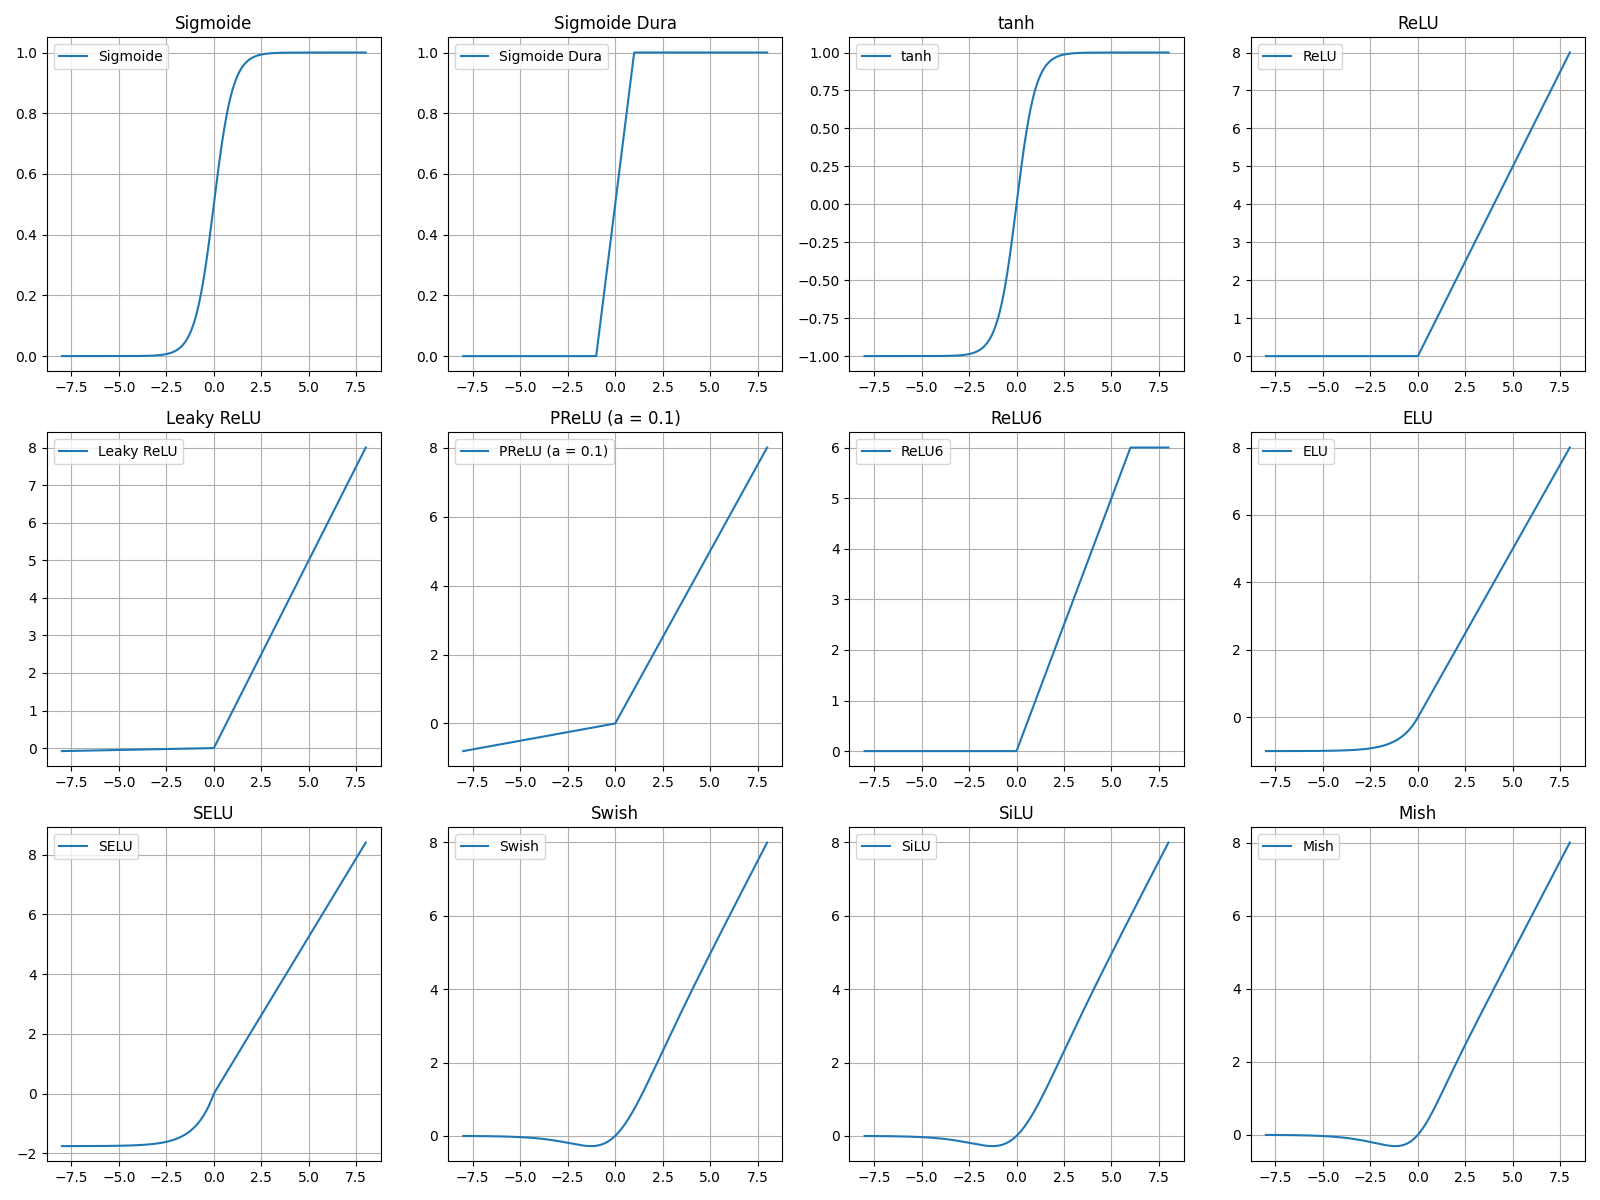
\includegraphics[width=0.7\textwidth]{activation_functions.png}
    \caption{Ejemplos de funciones de activación comunes.}
    \label{fig:activation_functions}
\end{figure}

\section{Redes Neuronales Profundas}

Las redes neuronales profundas (Deep Neural Networks, DNN) son un tipo de red neuronal que tiene múltiples capas ocultas entre la capa de entrada y la capa de salida. La profundidad de estas redes les permite aprender características complejas a diferentes niveles de abstracción. Han demostrado un rendimiento excepcional en tareas como el reconocimiento de voz, la visión por computadora y la traducción automática.

\begin{figure}[h]
    \centering
    \includegraphics[width=0.7\textwidth]{deep_neural_network.png}
    \caption{Estructura de una red neuronal profunda.}
    \label{fig:deep_neural_network}
\end{figure}

\section{Aplicaciones de las Redes Neuronales}

Las redes neuronales tienen una amplia gama de aplicaciones en diversos campos, incluyendo:

\begin{itemize}
    \item \textbf{Visión por Computadora:} Utilizadas para tareas como la clasificación de imágenes, la detección de objetos y la segmentación de imágenes.
    \item \textbf{Procesamiento del Lenguaje Natural (NLP):} Empleadas en la traducción automática, la generación de texto y el análisis de sentimientos.
    \item \textbf{Reconocimiento de Voz:} Implementadas en sistemas de reconocimiento y síntesis de voz.
    \item \textbf{Finanzas:} Utilizadas para la predicción de precios de acciones y la detección de fraudes.
\end{itemize}

\begin{figure}[h]
    \centering
    \includegraphics[width=0.7\textwidth]{nn_applications.png}
    \caption{Áreas de aplicación de las redes neuronales.}
    \label{fig:nn_applications}
\end{figure}

\section{Desafíos y Tendencias Futuras}

A pesar de los éxitos de las redes neuronales, existen desafíos que todavía deben ser abordados, como la interpretación de modelos, el requerimiento de grandes cantidades de datos para el entrenamiento y el consumo de recursos computacionales. Sin embargo, el campo está en constante evolución, con investigaciones en áreas como las redes neuronales convolucionales (CNN), las redes neuronales recurrentes (RNN) y los modelos generativos, que prometen avances significativos en el futuro.


























\section{Métodos de Optimización} NO


La optimización se refiere a la tarea de minimizar o maximizar una función $f(x)$ modificando $x$. En general, la optimización alude a una minimización, ya que la maximización es equivalente a la minimización de $-f(x)$. La función a minimizar (o maximizar) se conoce como función objetivo o criterio, que se utiliza para evaluar una solución candidata, por ejemplo, los pesos en una red neuronal. Cuando se está minimizando, según Goodfellow y col. (2016), se le denomina también función de coste (\textit{cost function}), función de pérdida (\textit{loss function}), o función de error (\textit{error function}). La función de pérdida es necesaria para poder disponer de un error que retropropagar durante la etapa de aprendizaje. Así pues, la función o grupo de funciones que se están minimizando se denominan \textit{loss functions}, y el valor que obtiene la minimización o maximización se identifica con el símbolo $\hat{x} = \arg \min f(x)$.

Conviene destacar que la función de pérdida debe ser diferenciable, y en este sentido, durante el entrenamiento, mediante dicha función se compara la salida de la red neuronal (predicción) con la etiqueta del objetivo verdadera (\textit{ground-truth}). Según los distintos modelos de red, se definen diferentes funciones de pérdida. En la red neuronal se obtienen todos los cálculos realizados por cada una de las capas. Por tanto, si cada uno de estos cálculos es diferenciable, entonces la función de pérdida también será diferenciable. No obstante, a veces se utilizan funciones de activación, tales como ReLU, que no son diferenciables; en estos casos es necesario aplicar alguna aproximación derivativa para poder utilizar la función en los procesos de retropropagación, mediante gradiente descendente, como se verá posteriormente.

Una función de pérdida es una medida de cuán bueno es un modelo de predicción en términos de poder aproximarse lo más posible (predecir) al resultado esperado. Uno de los métodos más utilizados para encontrar el punto mínimo de una función es el denominado \textit{descenso de gradiente}. Se puede pensar en la función de pérdida como una montaña ondulada y el descenso en pendiente es como deslizarse por la montaña para llegar al punto más bajo; de aquí surge el concepto de optimización mediante el gradiente (\textit{gradient-based optimization}). Cuando se calcula la pérdida, se debe mejorar el modelo. Esto se hace propagando el error hacia atrás a través de la estructura del modelo, de forma que en las redes neuronales son los pesos del modelo los que terminan ajustándose. Esto cierra el ciclo de aprendizaje entre el envío de los datos hacia adelante, la generación de predicciones y la mejora durante la propagación hacia atrás. Al adaptar los pesos, el modelo probablemente mejore (a veces mucho, a veces ligeramente) y, por lo tanto, se dice que se ha realizado el aprendizaje.

Resulta bien conocido que la derivada de una función en un punto $x$ proporciona la pendiente de la función en dicho punto. La derivada permite escalar un pequeño cambio en la entrada para obtener el correspondiente cambio en la salida: $f(x+\delta) = f(x) + \delta f'(x)$. La derivada es, por tanto, útil para minimizar una función porque indica cómo cambiar $x$ para conseguir una pequeña mejora en la salida $y$. Por ejemplo, se sabe que $f(x - \delta \cdot \text{sign}(f'(x)))$ es menor que $f(x)$ para un $\delta$ suficientemente pequeño. Se puede entonces disminuir $f(x)$ moviéndose en pequeños pasos con el signo opuesto de la derivada. Esto se conoce como \textit{gradiente descendente} (\textit{gradient descent}).

\begin{figure}[h!]
    \centering
    \includegraphics[width=0.5\textwidth]{gradiente_descendente.png}
    \caption{Gradiente descendente}
    \label{fig:gradiente}
\end{figure}

Para $x < 0$, $f'(x) < 0$ y $f$ disminuye hacia la derecha. Para $x > 0$, $f'(x) > 0$ y $f$ disminuye hacia la izquierda. Para $x = 0$, el gradiente se detiene puesto que $f'(x) = 0$.

Cuando $f'(x) = 0$, la derivada no proporciona información sobre la dirección en la que hay que moverse, de esta forma, los puntos con $f'(x) = 0$ se conocen como puntos críticos o puntos estacionarios. Un mínimo local es un punto donde $f(x)$ es menor que todos los puntos vecinos, de modo que no es posible disminuir $f(x)$ mediante pasos infinitesimales. Un máximo local es un punto donde $f(x)$ es mayor que todos los puntos vecinos, de modo que no es posible incrementar $f(x)$ mediante pasos infinitesimales. Otros puntos críticos denominados puntos de inflexión son los que tienen vecinos que son mayores y menores que el punto mismo, pero no son ni máximos ni mínimos.

\begin{figure}[h!]
    \centering
    \includegraphics[width=0.5\textwidth]{puntos_criticos.png}
    \caption{Puntos críticos}
    \label{fig:puntos_criticos}
\end{figure}

Un punto que obtiene el valor más bajo de $f(x)$ es un mínimo global. Puede haber solo un mínimo global o múltiples mínimos globales de la función. También es posible que haya mínimos locales que no sean globalmente óptimos. En el contexto del aprendizaje profundo, se optimizan las funciones que pueden tener muchas limitaciones locales que no son óptimas y muchos puntos de inflexión rodeados de regiones muy planas. Todo esto hace que la optimización sea difícil, especialmente cuando la entrada a la función es multidimensional.

A menudo es necesario minimizar funciones que tienen múltiples ($n$) entradas: $f: \mathbb{R}^n \to \mathbb{R}$, con una única salida (escalar). Con múltiples entradas, se debe utilizar el concepto de derivadas parciales $\frac{\partial f(x)}{\partial x_i}$, que mide cómo cambia $f$ según aumenta la variable $x_i$ en el punto $x$. El gradiente generaliza la noción de derivada al caso en que la derivada es con respecto a un vector: el gradiente de $f$ es el vector que contiene todas las derivadas parciales, denotado por $\nabla f(x)$. El elemento $i$-ésimo del gradiente es la derivada parcial de $f$ con respecto a $x_i$. En múltiples dimensiones, los puntos críticos son puntos en los que cada elemento del gradiente es igual a cero. La derivada direccional en la dirección $u$ (vector unitario) es la pendiente de la función $f$ en esa dirección $u$. En otras palabras, la derivada direccional es la derivada de la función $f(x + \alpha u)$ con respecto a $\alpha$, evaluada en $\alpha = 0$. Usando la regla de la cadena, se determina que $f(x + \alpha u)$ evalúa $u \cdot \nabla f(x)$ cuando $\alpha = 0$.

Para minimizar $f$, es deseable encontrar la dirección en la que $f$ disminuye de forma más rápida, lo que se puede hacer usando la derivada direccional:
\[
\min_u \nabla f(x) \cdot u = \min_{\theta} \|\nabla f(x)\| \cos(\theta)
\]
donde $\theta$ es el ángulo entre $u$ y el gradiente. Sustituyendo $\|u\| = 1$ e ignorando factores que no dependen de $\theta$, se concreta en minimizar $\min_{u} \cos \theta$. Esto se consigue cuando $u$ apunta en la dirección opuesta del gradiente. En otras palabras, el gradiente apunta directamente hacia arriba. Se puede hacer decrecer $f$ moviéndose en la dirección opuesta del gradiente, lo que se conoce como método del gradiente descendente (\textit{steepest descent} o \textit{gradient descent}), que propone un nuevo punto,
\[
x' = x - \eta \nabla f(x)
\]
donde $\eta$ es la razón de aprendizaje, que es un valor escalar que determina la dimensión del paso. Se puede elegir de varias formas, una de ellas es fijarlo a un valor pequeño constante. Algunas veces se puede determinar la dimensión del paso que hace desaparecer la derivada direccional. Otra aproximación consiste en evaluar $f(x - \eta \nabla f(x))$ para varios valores de $\eta$ y elegir el que proporciona el valor de la función objetivo más pequeño. Esta estrategia se denomina \textit{búsqueda en línea} (\textit{line search}).

El gradiente descendente converge cuando cada elemento del gradiente es cero (o, en la práctica, muy próximo a cero). En algunos casos, se puede evitar ejecutar este algoritmo iterativo y simplemente saltar al punto en el que el gradiente es igual a cero. En muchas situaciones es posible resolver analíticamente la ecuación $\nabla f(x) = 0$. En la optimización convexa, la optimización de funciones cóncavas y diferenciables que tienen una única solución óptima global, se puede obtener una solución cerrada sin necesidad de recurrir a métodos iterativos, como el gradiente descendente. Sin embargo, las redes neuronales, así como otros modelos que pueden tener múltiples óptimos locales y limitaciones no convexas, se enfrentan a mayores desafíos en este aspecto.



\subsection{Gradiente Descendente Estocástico}

En el ámbito del aprendizaje automático, el problema del Gradiente Descendente Estocástico (SGD, Stochastic Gradient Descent) consiste en minimizar una función objetivo que tiene la forma (Bishop, 2006; Ruder, 2017),

\begin{equation}
J(w) = \sum_{i=1}^{n} L(y_i, f(x_i; w)),
\end{equation}

donde el parámetro \( w \), que minimiza \( J(w) \), debe estimarse. \( J_i \) se asocia con la i-ésima observación en el conjunto de datos utilizados para el entrenamiento (ajuste). El término estocástico proviene del hecho relativo a la selección de las muestras (observaciones) para el ajuste de forma aleatoria, que incluso se pueden seleccionar por lotes en cada iteración. \( J(w) \) es el valor de la función de pérdida (loss function) en el i-ésimo ejemplo y \( J(w) \) es el riesgo empírico.

El gradiente descendente se usa para minimizar la siguiente función de forma iterativa, con iteraciones \( t \). En el Anexo se proporciona un mayor nivel de detalle.

\begin{equation}
w(t+1) = w(t) - \eta \nabla J(w(t)),
\end{equation}

donde \( \eta \) es la tasa de aprendizaje. De esta forma iterativa, el método recorre el conjunto de entrenamiento y realiza la actualización indicada anteriormente para cada muestra de entrenamiento. Según la ecuación (2.5), gradientes negativos incrementan el peso y viceversa, siempre con el fin de minimizar la función objetivo. Se pueden realizar varios pasos sobre el conjunto de entrenamiento hasta que el algoritmo converja. Si se hace esto, los datos se pueden seleccionar aleatoriamente en cada paso para evitar ciclos; es lo que se conoce como criterio estocástico. Estas muestras así seleccionadas constituyen lo que se denomina un lote (batch). Las implementaciones típicas pueden usar una razón de aprendizaje adaptativa para que el algoritmo converja.

En pseudocódigo, el método del gradiente descendente estocástico es como sigue:

\begin{enumerate}
    \item Elegir un vector inicial de parámetros \( w \) (puede ser aleatoriamente) y una tasa de aprendizaje \( \eta \).
    \item Repetir hasta que se consiga un mínimo aproximado:
    \begin{enumerate}
        \item Seleccionar aleatoriamente ejemplos en el conjunto de entrenamiento.
        \item Para \( i = 1, 2, \ldots, n \), hacer:
        \begin{equation}
        w(t+1) = w(t) - \eta \nabla J_i(w).
        \end{equation}
    \end{enumerate}
\end{enumerate}

\subsection{Ejemplo}

Supóngase que se quiere ajustar una línea recta \( y = w_1 + w_2 x \) a partir de un conjunto de observaciones \( (x_1, x_2, \ldots, x_n) \) con sus correspondientes respuestas estimadas \( (y_1, y_2, \ldots, y_n) \) utilizando mínimos cuadrados. La función objetivo a minimizar es:

\begin{equation}
J(w) = \sum_{i=1}^{n} (w_1 + w_2 x_i - y_i)^2.
\end{equation}

El punto 2.2 del pseudocódigo resulta en:

\begin{equation}

w_1(t+1) = w_1(t) - \eta \sum_{i=1}^{n} 2(w_1 + w_2 x_i - y_i),
\end{equation}

\begin{equation}
w_2(t+1) = w_2(t) - \eta \sum_{i=1}^{n} 2(w_1 + w_2 x_i - y_i)x_i.
\end{equation}

En cada iteración (también llamada actualización), solo se evalúa el gradiente en un único punto \( x \) en lugar de evaluar en el conjunto de todas las muestras. La diferencia clave en comparación con el gradiente descendente estándar es que solo se utiliza un dato del total del conjunto de datos disponible para obtener la actualización, y el dato se selecciona de forma aleatoria en cada paso.

Existen diversas variantes, extensiones y mejoras del algoritmo. Resulta de particular interés el hecho de fijar la razón de aprendizaje, ya que valores altos tienden hacia la divergencia de los datos, mientras que valores demasiado pequeños hacen que la convergencia sea lenta. Una forma de abordar este problema es que dicha razón sea variable disminuyendo a medida que se incorporan nuevas muestras (mayor aprendizaje). Esto se consigue haciéndola dependiente del número de datos o iteraciones. Una de tales extensiones es la del método del momentum (Rumelhart y col., 1986; Murphy 2012). Este método recuerda la actualización \( \Delta w \) en cada iteración, determinando la siguiente actualización como una combinación lineal del gradiente y la actualización previa (Sutskever y col., 2013):

\begin{equation}
\Delta w(t) = \alpha \Delta w(t-1) - \eta \nabla J_i(w(t-1)),
\end{equation}

\begin{equation}
w(t) = w(t-1) + \Delta w(t).
\end{equation}

En resumen, la dimensión del lote expresa el número de muestras procesadas antes de actualizar los pesos de la red. El número de épocas (epochs) es el número de pases completos de todo el conjunto de muestras de entrenamiento \( N \). Se puede establecer que la razón de aprendizaje varíe cada cierto número de épocas, por ejemplo, cada 5 épocas disminuye un 10\% con respecto al valor inicial. Se puede ejecutar el algoritmo todo el tiempo que se desee e incluso detenerlo utilizando otros criterios además de un número fijo de épocas, tal como que el error del modelo o que la función objetivo no cambia con el número de iteraciones. En estos casos se dice que se ha alcanzado la convergencia y los criterios así establecidos se denominan de convergencia.

A modo de ejemplo, supóngase un conjunto de datos con 400 muestras, de forma que se define la dimensión del lote en 10 con 100 épocas. Esto significa que el conjunto de datos se divide en 40 lotes, cada lote con 10 muestras. La actualización de los pesos del modelo se realizará tras el paso de cada lote con 10 muestras. Así, una época involucra 40 lotes, es decir, 40 actualizaciones del modelo.




Esto se consigue haciéndola dependiente del número de datos o iteraciones. Una de tales extensiones es la del método del \textit{momentum} (Rumelhart y col., 1986; Murphy, 2012). Este método recuerda la actualización $\Delta w$ en cada iteración, determinando la siguiente actualización como una combinación lineal del gradiente y la actualización previa (Sutskever y col., 2013):

\[
\Delta w(t) = \alpha \Delta w(t-1) - \eta \nabla J_i(w(t-1))
\]

La anterior expresión conduce a:

\[
w(t) = w(t-1) + \alpha \Delta w(t-1) - \eta \nabla J_i(w(t-1))
\]

donde $\eta > 0$ es la razón de aprendizaje y $\alpha \in [0,1]$ es la constante de momento que controla la velocidad de actualización de $\Delta w(t-1)$. El vector de parámetros, $w$, que minimiza $J(w)$ es realmente el que se estima en el proceso de optimización. El nombre de \textit{momentum} proviene del concepto de momento en física, de forma que el vector de pesos $w$, visto como una partícula viajando a través del espacio de parámetros, adquiere una aceleración a partir de la fuerza, tendiendo a mantenerse en la misma dirección, evitando así oscilaciones.

En los procesos de optimización de redes neuronales, si los gradientes incrementan su magnitud exponencialmente, por ejemplo, porque los pesos toman valores altos afectando a los resultados de las multiplicaciones, el entrenamiento se hace inestable y puede divergir en unas pocas iteraciones. Esto es lo que se conoce como \textit{explosión del gradiente}. Pascanu y col. (2013) proponen el \textit{recorte de gradiente} (\textit{gradient clipping}), que ayuda a prevenir dicha explosión estabilizando el entrenamiento ante la presencia de \textit{outliers}. Para ello se propone considerar un determinado umbral $T$ de forma que si:

\[
\|\nabla J(w)\| > T \text{ entonces } \nabla J(w) = T \frac{\nabla J(w)}{\|\nabla J(w)\|}
\]

De forma similar, si los valores del gradiente son muy pequeños también por influencia de valores de pesos pequeños, el problema se conoce como \textit{desaparición del gradiente}. En la literatura se han investigado diversas aproximaciones en aras de la mejora de la convergencia, por ejemplo, mediante el promediado de trayectorias (Polyak y Juditsky, 1992).

Durante el proceso de actualización de los pesos de la red, mediante el cálculo del error, existen básicamente tres tipos de estrategias. En todas ellas, se dispone de $N$ muestras de entrenamiento, la diferencia estriba en cómo se realiza la actualización (Kim, 2017; Brownlee, 2018). El proceso de optimización es iterativo, lo que quiere decir que cuando se busca el mínimo, se realizan una serie de pasos, siendo el objetivo de cada paso ajustar lo mejor posible los pesos. Cada paso consiste en utilizar el modelo con los parámetros actuales, realizar una predicción sobre algunas muestras, comparar las predicciones con las muestras, calcular el error y propagar el error hacia atrás para actualizar de nuevo los pesos del modelo.

Una muestra es un dato simple, también llamada instancia, observación, vector de entrada o vector de características, que se suministra al algoritmo junto con una salida que se utiliza para comparar el error con respecto a la salida que se obtiene con ella y la esperada. Este planteamiento se engloba en lo que se denomina \textit{aprendizaje supervisado}. Un conjunto de muestras de entrenamiento engloba un cierto número, $n$, de muestras.

Como se ha indicado anteriormente, existe el concepto de \textit{lote} (\textit{batch}) que define el número de muestras utilizadas antes de llevar a cabo una actualización de los pesos de la red en el modelo. Considérese un lote, constando de una o más muestras dentro de un bucle y haciendo predicciones precisamente con esas muestras del lote. Una vez que han pasado todas las muestras del lote, se realizan las predicciones y se comparan con las variables de salida esperadas para obtener el error correspondiente. Con este error, el algoritmo de optimización actualiza los pesos que definen el modelo. Esto significa que hasta que no han pasado todas las muestras del lote no se actualizan dichos pesos. Un conjunto de datos de entrenamiento se puede dividir en uno o más lotes.

Cuando todas las muestras de entrenamiento se utilizan para crear un lote, el algoritmo de aprendizaje se denomina \textit{descenso del gradiente por lotes}. Cuando el lote es del tamaño de una muestra, el algoritmo de aprendizaje se denomina \textit{descenso de gradiente estocástico} (\textit{SGD}) o de otro tipo. Cuando el tamaño del lote posee más de una muestra y es menor que el tamaño del conjunto de datos de entrenamiento, el algoritmo de aprendizaje se denomina \textit{descenso de gradiente de mini-lote} (\textit{mini-batch}). Dimensiones habituales de los mini-lotes son 32, 64 y 128, lo que suele derivar en el hecho de que el último lote a veces tiene un tamaño menor que el resto, al no coincidir el número de muestras totales con esas dimensiones, cuando se reparten las muestras en los lotes. A veces se eliminan algunas muestras para que esto no ocurra.

Por otra parte, existe otro parámetro conocido como \textit{época} (\textit{epoch}), que define el número de veces que el conjunto total de muestras son procesadas por el algoritmo. Esto significa que cada muestra del conjunto $N$ ha tenido una oportunidad de actualizar los pesos en cada \textit{epoch}. Una \textit{epoch} puede tener uno o más lotes. Para mayor claridad, se puede pensar en un bucle sobre el número de \textit{epochs} donde cada iteración o ciclo opera sobre $N$. Dentro de esta iteración, existe otra iteración anidada que actúa sobre cada lote de muestras, teniendo en cuenta que un lote tiene el número especificado de muestras según el tamaño del lote. El número de \textit{epochs} depende del tipo de datos, siendo a veces alto, para garantizar una eficiencia suficiente. Se pueden encontrar aplicaciones con 10, 100, 1000 e incluso más, y naturalmente también con menos. Además, es común representar gráficamente, sobre un sistema de ejes bidimensional (x-y), el proceso de aprendizaje mostrando las \textit{epochs} sobre el eje horizontal $x$ junto con las iteraciones y el error del modelo en el eje $y$. Estas representaciones ayudan a diagnosticar la evolución del aprendizaje, y cómo el modelo se ajusta adecuadamente o no al conjunto de datos de entrenamiento.

En resumen, la dimensión del lote expresa el número de muestras procesadas antes de actualizar los pesos de la red. El número de \textit{epochs} es el número de pases completos de todo el conjunto de muestras de entrenamiento $N$. Se puede establecer que la razón de aprendizaje varíe cada cierto número de \textit{epochs}, por ejemplo, cada 5 \textit{epochs} disminuya un 10\% con respecto al valor inicial. Se puede ejecutar el algoritmo todo el tiempo que se desee e incluso detenerlo utilizando otros criterios además de un número fijo de \textit{epochs}, tal como que el error del modelo o que la función objetivo no cambia con el número de iteraciones. En estos casos se dice que se ha alcanzado la convergencia y los criterios así establecidos se denominan de convergencia. A modo de ejemplo, supóngase un conjunto de datos con 400 muestras, de forma que se define la dimensión del lote en 10 con 100 \textit{epochs}. Esto significa que el conjunto de datos se divide en 40 lotes, cada lote con 10 muestras. La actualización de los pesos del modelo se realizará tras el paso de cada lote con 10 muestras. Así, una \textit{epoch} involucra 40 lotes, es decir, 40 actualizaciones del modelo.

A veces ocurre que el conjunto de muestras de entrenamiento no es divisible por un determinado número de lotes, en este caso cabe la posibilidad de considerar el último lote con menos muestras que los otros, como se ha indicado previamente, o bien eliminar algunas muestras del conjunto de datos o también cambiar el tamaño del lote. Supóngase que se tiene un conjunto de muestras de entrenamiento de 208, y se establece la dimensión del mini-lote en 10 con 4 \textit{epochs}, esto significa que el paso de las 208 muestras determina una \textit{epoch}. El número de mini-lotes se obtiene calculando el resultado de la división $208/10 = 20.8$, lo que significa que se formarán 20 mini-lotes con 10 muestras cada uno, más uno adicional con 8 muestras. En total habrá 21 mini-lotes. Cada uno de estos mini-lotes define una iteración, por lo que en cada \textit{epoch} se realizan 21 iteraciones, de forma que tras cada una de ellas se actualizan los pesos.

Considerando la ecuación (2.9) simplificada $\Delta w = -\eta \nabla J_i(w(t-1))$ y un conjunto con $N$ muestras de entrenamiento, cuando no se definen mini-lotes, o lo que es lo mismo, la dimensión del mini-lote es 1, entonces, cada muestra actualiza los pesos según esta ecuación. Por el contrario, si las $N$ muestras forman un lote, entonces la actualización de los pesos se realiza una única vez, promediando los pesos obtenidos tras el paso de cada muestra como sigue:

\[
\Delta w = \frac{1}{N} \sum_{k=1}^{N} \Delta w(k)
\]

Si se establecen mini-lotes de dimensión $m$, la actualización de los pesos también se lleva a cabo de la misma manera que en el caso anterior, si bien promediando con $m$ en lugar de $N$ y realizando tantas actualizaciones por \textit{epoch} como número de mini-lotes existan.





























¿QUITAR?
La ecuación \ref{eq:conv} resume las explicaciones anteriores en una gran ecuación matemática \citep{pajares2021aprendizaje}:

\begin{equation}
z_{i,j,k} = b_k + \sum_{u=0}^{f_h-1} \sum_{v=0}^{f_w-1} \sum_{k'=0}^{f_n'-1} x_{i',j',k'} \cdot w_{u,v,k',k} \hspace{5mm} \textup{con }
\left\{
\begin{array}{l}
i' = i \cdot s_h + u \\
j' = j \cdot s_w + v
\end{array}
\right.
\end{equation} \label{eq:conv}

donde \( z_{i,j,k} \) es la salida de la neurona ubicada en \((i,j)\) en el mapa de características \(k\) de la capa convolucional \(l\). \( s_h \) y \( s_w \) es el stride vertical y horizontal. \( f_h \) y \( f_w \) son las dimensiones del campo receptivo y \( f_{n'} \) es el número de mapas de características de la capa anterior. \( x_{i',j',k'} \) es la salida de la neurona situada en \((i',j')\) y en mapa de características \(k'\). \( b_k \) es el término de sesgo para el mapa de características \(k\) en la capa \(l\) y \( w_{u,v,k',k} \) es el peso de conexión entre cualquier neurona del mapa de características \(k\) de la capa \(l\) y su entrada en \((u,v)\) y el mapa de características \(k'\).


























Una de las redes neuronales más importantes y más utilizadas en el campo de la ciberseguridad son las \acrfull{cnn}. Las CNN tienen su origen en el estudio de la corteza visual del cerebro y han sido utilizadas en el reconocimiento de imágenes desde la década de los 80. Actualmente, debido al aumento en la capacidad computacional, la disponibilidad de grandes volúmenes de datos de entrenamiento y las técnicas avanzadas de redes profundas, han permitido que las CNN alcancen un rendimiento excepcional en tareas visuales complejas. Estas redes son la base de servicios como la búsqueda de imágenes o los vehículos autónomos \citep{geron2022hands}.


Una \acrfull{cnn} es una red neuronal diseñada para procesar entradas almacenadas en matrices. Un ejemplo de entrada es una imagen en escala de grises, que es una matriz bidimensional (2D) de píxeles. Aunque estas redes se utilicen principalmente en la clasificación visual de imágenes, también  se han demostrado que son efectivas en tareas como el reconocimiento de voz (matrices 2D de imágenes o espectrogramas de audio) \citep{kim2023bilstm}, clasificación visual de videos o imágenes volumétricas (matrices tridimensionales 3D) \citep{diba2017temporal} y procesamiento de lenguaje natural(matriz 2D) \citep{wang2017combining}. Independientemente de la dimensionalidad, las CNN se utilizan donde hay un ordenamiento espacial o temporal \citep{berman2019survey}. No obstante, nos enfocaremos únicamente en sus aplicaciones visuales.

La arquitectura de una CNN (ver Figura ????????) consta de tres tipos distintos de capas: capas de convolución, capas de pooling y la capa de clasificación. 

IMAGEN CAPAS: \citep{phung2018deep}


\subsubsection*{Capas convolucionales}

La capa convolucional es el bloque de construcción más importante de una red neuronal convolucional (CNN). En ella se aplica la operación de convolución, que involucra dos funciones y produce una tercera función que representa la cantidad de superposición de una función a medida que se desplaza sobre otra. Supóngase que se tiene una fuente de luz variable cuya intensidad se recibe mediante un sensor. Este sensor proporciona una salida en una determinada posición \( x \) en el tiempo \( t \), esto es, \( x(t) \). Tanto \( x \) como \( t \) son valores reales, de forma que debido a la variabilidad de la fuente mencionada, se pueden obtener diferentes lecturas en diferentes instantes de tiempo. La captura de la señal por el sensor puede estar contaminada con cierto ruido. Para obtener una señal más limpia, lo acertado es realizar un promediado de la salida con varias medidas. Si además tenemos en cuenta que las medidas más recientes son más relevantes que las alejadas en el tiempo, el promediado puede ponderarse concediendo más relevancia a las medidas recientes. Esto puede hacerse mediante una función de promediado \( w(a) \), donde \( a \) representa el alejamiento de la medida en el tiempo. Si se realiza esta operación de promediado ponderado en cada instante de tiempo \( t \), se obtiene una nueva función promediada como sigue:

\begin{equation}
s(t) = \int x(a) w(t-a) \, da
\end{equation}

Esta operación se denomina convolución, y se denota como:

\begin{equation}
s(t) = \int (x \star w)(t)
\end{equation}

Para que el promedio ponderado sea válido, la función de promediado \( w(t) \) necesita ser una función de densidad de probabilidad. Además, \( w(t) \) debe ser cero para todos los valores negativos de \( t \) para evitar tomar valores futuros, lo cual no es físicamente posible \citep{pajares2021aprendizaje}.


Para aplicaciones prácticas como el procesamiento de imágenes, las medidas suelen ser discretas, es decir, se toman en intervalos de tiempo específicos. En este caso, el tiempo \( t \) toma valores enteros, y la convolución discreta se define como:

\begin{equation}
s(t) = (x \star w)(t) = \sum_{a=-\infty}^{\infty} x(a) w(t-a)
\end{equation}

En el contexto de las CNN, la entrada es un vector o matriz multidimensional de datos (la imagen), y el núcleo es una matriz multidimensional de parámetros que se ajustan durante el proceso de aprendizaje. Sea \( I \) la imagen de entrada y \( K \) un núcleo de convolución. Se define la convolución discreta en dos dimensiones como:

\begin{equation}
S(i, j) = (K \star I)(i, j) = \sum_{m=0}^{M-1} \sum_{n=0}^{N-1} I(i+m, j+n) K(m, n)
\end{equation}

donde \( M \) y \( N \) son las dimensiones del núcleo. La figura ????? muestra un ejemplo de convolución con el núcleo \( K \), aplicado sobre una imagen \( I \). 


En una CNN, esta construcción es la mas importante. Las neuronas de la primera capa convolucional se concectan a todos y cada uno de los píxeles de la imagen de entrada, sino solo a píxeles en sus campos receptivos. A su vez, cada neurona de la segunda capa convolucional está conectada a las neuronas ubicadas dentro de un rectángulo pequeño en la primera capa. Esta arquitectura permite a la red concentrarse en cracterísticas pequeñas de bajo nivel en la primera capa oculta, juntarlas después para crear características más grandes de nivel superior en la siguiente capa oculta, y así sucesivamente. La convolución se realiza con solapamiento total del núcleo, lo que resulta en una imagen resultante de menor dimensión (REFERENCIA IMAGEN A ?????). Si se desea mantener la misma dimensión, se puede aplicar relleno con ceros o zero-padding (REFERENCIA IMAGEN A ?????). Este relleno se indica como "same" en términos de implementación. Si no se realiza relleno con ceros, se indica como "valid". Por otra parte, en las convoluciones, el campo receptivo se define como la región de entrada que contribuye a la salida generada por el filtro. En la figura REFERENCIA IMAGEN A ?????) se muestran sendos campos receptivos de la imagen \( I \) que contribuyen a las salidas \( P \) y \( \Q \) generadas por el filtro \( K \).


IMAGENES PADDING

Por último, se define el stride. Stride es la longitud de paso de desplazamiento del núcleo alrededor de la entrada. Cuando la longitud de paso es 1, el núcleo se desplaza sobre la entrada un elemento a la vez. Normalmente, la longitud de paso se establece de manera que el volumen de salida sea un número entero.

FOTOOO stride Fuente:\citep{yepez2020stride}

La Figura de la izquierda muestra una entrada de \(5 \times 5\) con un núcleo de \(3 \times 3\). Con un stride de paso 1, se genera una matriz de salida de tamaño \(3 \times 3\). Una longitud de paso de 1 se utiliza normalmente para extraer el máximo número de características, ya que proporciona el máximo solapamiento entre el núcleo y la entrada, pero a máxima complejidad computacional. Por otro lado, la imagen de la derecha muestra el núcleo desplazándose dos unidades sobre la entrada, generando una matriz de salida de \(2 \times 2\). Generalmente, cuando la longitud de paso es mayor que 1, los campos receptivos se solapan menos y producen una salida más pequeña. Si la longitud de paso fuera 3, habría problemas con el espaciado, ya que el campo receptivo no encajaría alrededor de la entrada como un número entero \citep{yepez2020stride}.









cada neurona en la capa convolucional está conectada solo a una pequeña región de la imagen de entrada (campo receptivo). Estas conexiones se realizan utilizando filtros (o núcleos de convolución), y la salida se conoce como mapa de características. La ecuación \ref{eq:conv} resume las explicaciones anteriores en una gran ecuación matemática \citep{pajares2021aprendizaje}:

\begin{equation}
z_{i,j,k} = b_k + \sum_{u=0}^{f_h-1} \sum_{v=0}^{f_w-1} \sum_{k'=0}^{f_n'-1} x_{i',j',k'} \cdot w_{u,v,k',k} \hspace{5mm} \textup{con }
\left\{
\begin{array}{l}
i' = i \cdot s_h + u \\
j' = j \cdot s_w + v
\end{array}
\right.
\end{equation}

donde:
\begin{itemize}
    \item \( z_{i,j,k} \) es la salida de la neurona ubicada en la fila \(i\), columna \(j\) en el mapa de características \(k\) de la capa convolucional (capa \(l\)).
    \item \( s_h \) y \( s_w \) son los pasos de avance vertical y horizontal.
    \item \( f_h \) y \( f_w \) son la altura y la anchura del campo receptivo y \( f_{n'} \) es el número de mapas de características de la capa anterior (capa \(l-1\)).
    \item \( x_{i',j',k'} \) es la salida de la neurona situada en la fila \(i'\), columna \(j'\), mapa de características \(k'\) (o canal \(k'\) si la capa anterior es la capa de entrada).
    \item \( b_k \) es el término de sesgo para el mapa de características \(k\) (en la capa \(l\)). Puedes imaginarlo como una rueda que ajusta el brillo general del mapa de características \(k\).
    \item \( w_{u,v,k',k} \) es el peso de conexión entre cualquier neurona del mapa de características \(k\) de la capa \(l\) y su entrada situada en la fila \(u\), columna \(v\) (relativa al campo receptivo de la neurona) y el mapa de características \(k'\).
\end{itemize}









\subsection{Red Neuronal Convolucional}

Una de las redes neuronales más importantes y más utilizadas en el campo de la ciberseguridad son las \acrfull{cnn}. Las CNN tienen su origen en el estudio de la corteza visual del cerebro y han sido utilizadas en el reconocimiento de imágenes desde la década de los 80. Actualmente, debido al aumento en la capacidad computacional, la disponibilidad de grandes volúmenes de datos de entrenamiento y las técnicas avanzadas de redes profundas, han permitido que las CNN alcancen un rendimiento excepcional en tareas visuales complejas. Estas redes son la base de servicios como la búsqueda de imágenes o los vehículos autónomos \citep{geron2022hands}.

Una \acrfull{cnn} es una red neuronal diseñada para procesar entradas almacenadas en matrices. Un ejemplo de entrada es una imagen en escala de grises, que es una matriz bidimensional (2D) de píxeles. Aunque estas redes se utilicen principalmente en la clasificación visual de imágenes, también se ha demostrado que son efectivas en tareas como el reconocimiento de voz (matrices 2D de imágenes o espectrogramas de audio) \citep{kim2023bilstm}, clasificación visual de videos o imágenes volumétricas (matrices tridimensionales 3D) \citep{diba2017temporal} y procesamiento de lenguaje natural (matriz 2D) \citep{wang2017combining}. Independientemente de la dimensionalidad, las CNN se utilizan donde hay un ordenamiento espacial o temporal \citep{berman2019survey}. No obstante, nos enfocaremos únicamente en sus aplicaciones visuales.

La arquitectura de una CNN (ver Figura ????????) consta de tres tipos distintos de capas: capas de convolución, capas de pooling y la capa de clasificación.

\begin{figure}[h]
    \centering
    \includegraphics[width=0.8\textwidth]{path_to_image}
    \caption{Arquitectura de una CNN con capas de convolución, pooling y clasificación \citep{phung2018deep}.}
    \label{fig:cnn_architecture}
\end{figure}

\subsubsection*{Capas convolucionales}

La capa convolucional es el bloque de construcción más importante de una \fullacr{cnn}. En ella se aplica la operación de convolución, que involucra dos funciones y produce una tercera función que representa la cantidad de superposición de una función a medida que se desplaza sobre otra. Supóngase que se tiene una fuente de luz variable cuya intensidad se recibe mediante un sensor. Este sensor proporciona una salida en una determinada posición \( x \) en el tiempo \( t \), esto es, \( x(t) \). Tanto \( x \) como \( t \) son valores reales, de forma que debido a la variabilidad de la fuente mencionada, se pueden obtener diferentes lecturas en diferentes instantes de tiempo. La captura de la señal por el sensor puede estar contaminada con cierto ruido. Para obtener una señal más limpia, lo acertado es realizar un promediado de la salida con varias medidas. Si además tenemos en cuenta que las medidas más recientes son más relevantes que las alejadas en el tiempo, el promediado puede ponderarse concediendo más relevancia a las medidas recientes. Esto puede hacerse mediante una función de promediado \( w(a) \), donde \( a \) representa el alejamiento de la medida en el tiempo. Si se realiza esta operación de promediado ponderado en cada instante de tiempo \( t \), se obtiene una nueva función promediada como sigue:

\begin{equation}
s(t) = \int x(a) w(t-a) \, da
\end{equation}

Esta operación se denomina convolución, y se denota como:

\begin{equation}
s(t) = \int (x \star w)(t)
\end{equation}

Para que el promedio ponderado sea válido, la función de promediado \( w(t) \) necesita ser una función de densidad de probabilidad. Además, \( w(t) \) debe ser cero para todos los valores negativos de \( t \) para evitar tomar valores futuros, lo cual no es físicamente posible \citep{pajares2021aprendizaje}.


Para aplicaciones prácticas como el procesamiento de imágenes, las medidas suelen ser discretas, es decir, se toman en intervalos de tiempo específicos. En este caso, el tiempo \( t \) toma valores enteros, y la convolución discreta se define como:

\begin{equation}
s(t) = (x \star w)(t) = \sum_{a=-\infty}^{\infty} x(a) w(t-a)
\end{equation}

En el contexto de las CNN, la entrada es un vector o matriz multidimensional de datos (la imagen), y el núcleo es una matriz multidimensional de parámetros que se ajustan durante el proceso de aprendizaje. Sea \( I \) la imagen de entrada y \( K \) un núcleo de convolución. Se define la convolución discreta en dos dimensiones como:

\begin{equation}
S(i, j) = (K \star I)(i, j) = \sum_{m=0}^{M-1} \sum_{n=0}^{N-1} I(i+m, j+n) K(m, n)
\end{equation}

donde \( M \) y \( N \) son las dimensiones del núcleo. La figura \ref{fig:conv_example} muestra un ejemplo de convolución con el núcleo \( K \), aplicado sobre una imagen \( I \).

\begin{figure}[h]
    \centering
    \includegraphics[width=0.8\textwidth]{path_to_image}
    \caption{Ejemplo de convolución con un núcleo \( K \) aplicado sobre una imagen \( I \).}
    \label{fig:conv_example}
\end{figure}

En una CNN, esta construcción es la más importante. Las neuronas de la primera capa convolucional no se conectan a todos y cada uno de los píxeles de la imagen de entrada, sino solo a píxeles en sus campos receptivos. A su vez, cada neurona de la segunda capa convolucional está conectada a las neuronas ubicadas dentro de un rectángulo pequeño en la primera capa. Esta arquitectura permite a la red concentrarse en características pequeñas de bajo nivel en la primera capa oculta, juntarlas después para crear características más grandes de nivel superior en la siguiente capa oculta, y así sucesivamente. La convolución se realiza con solapamiento total del núcleo, lo que resulta en una imagen resultante de menor dimensión (ver Figura \ref{fig:padding_valid}). Si se desea mantener la misma dimensión, se puede aplicar relleno con ceros o zero-padding (ver Figura \ref{fig:padding_same}). Este relleno se indica como "same" en términos de implementación. Si no se realiza relleno con ceros, se indica como "valid". Por otra parte, en las convoluciones, el campo receptivo se define como la región de entrada que contribuye a la salida generada por el filtro. En la figura \ref{fig:receptive_field} se muestran sendos campos receptivos de la imagen \( I \) que contribuyen a las salidas \( P \) y \( Q \) generadas por el filtro \( K \).

\begin{figure}[h]
    \centering
    \includegraphics[width=0.8\textwidth]{path_to_image}
    \caption{Convolución con relleno "valid".}
    \label{fig:padding_valid}
\end{figure}

\begin{figure}[h]
    \centering
    \includegraphics[width=0.8\textwidth]{path_to_image}
    \caption{Convolución con relleno "same".}
    \label{fig:padding_same}
\end{figure}

\begin{figure}[h]
    \centering
    \includegraphics[width=0.8\textwidth]{path_to_image}
    \caption{Campos receptivos en una convolución.}
    \label{fig:receptive_field}
\end{figure}

Por último, se define el stride. Stride es la longitud de paso de desplazamiento del núcleo alrededor de la entrada. Cuando la longitud de paso es 1, el núcleo se desplaza sobre la entrada un elemento a la vez. Normalmente, la longitud de paso se establece de manera que el volumen de salida sea un número entero.

\begin{figure}[h]
    \centering
    \includegraphics[width=0.8\textwidth]{path_to_image}
    \caption{Ejemplo de convolución con diferentes strides. Fuente: \citep{yepez2020stride}.}
    \label{fig:stride_example}
\end{figure}

La Figura \ref{fig:stride_example} de la izquierda muestra una entrada de \(5 \times 5\) con un núcleo de \(3 \times 3\). Con un stride de paso 1, se genera una matriz de salida de tamaño \(3 \times 3\). Una longitud de paso de 1 se utiliza normalmente para extraer el máximo número de características, ya que proporciona el máximo solapamiento entre el núcleo y la entrada, pero a máxima complejidad computacional. Por otro lado, la imagen de la derecha muestra el núcleo desplazándose dos unidades sobre la entrada, generando una matriz de salida de \(2 \times 2\). Generalmente, cuando la longitud de paso es mayor que 1, los campos receptivos se solapan menos y producen una salida más pequeña. Si la longitud de paso fuera 3, habría problemas con el espaciado, ya que el campo receptivo no encajaría alrededor de la entrada como un número entero.



La ecuación \ref{eq:conv} resume las explicaciones anteriores en una gran ecuación matemática \citep{pajares2021aprendizaje}:

\begin{equation}
z_{i,j,k} = b_k + \sum_{u=0}^{f_h-1} \sum_{v=0}^{f_w-1} \sum_{k'=0}^{f_n'-1} x_{i',j',k'} \cdot w_{u,v,k',k} \hspace{5mm} \textup{con }
\left\{
\begin{array}{l}
i' = i \cdot s_h + u \\
j' = j \cdot s_w + v
\end{array}
\right.
\end{equation}

donde:
\begin{itemize}
    \item \( z_{i,j,k} \) es la salida de la neurona ubicada en la fila \(i\), columna \(j\) en el mapa de características \(k\) de la capa convolucional (capa \(l\)).
    \item \( s_h \) y \( s_w \) son los pasos de avance vertical y horizontal.
    \item \( f_h \) y \( f_w \) son la altura y la anchura del campo receptivo y \( f_{n'} \) es el número de mapas de características de la capa anterior (capa \(l-1\)).
    \item \( x_{i',j',k'} \) es la salida de la neurona situada en la fila \(i'\), columna \(j'\), mapa de características \(k'\) (o canal \(k'\) si la capa anterior es la capa de entrada).
    \item \( b_k \) es el término de sesgo para el mapa de características \(k\) (en la capa \(l\)).
    \item \( w_{u,v,k',k} \) es el peso de conexión entre cualquier neurona del mapa de características \(k\) de la capa \(l\) y su entrada situada en la fila \(u\), columna \(v\) (relativa al campo receptivo de la neurona) y el mapa de características \(k'\).
\end{itemize}


























Dentro del AA se encuadra el conocido como Aprendizaje Profundo (AP). En la literatura especializada a nivel internacional es muy común referirse al AP por sus términos en inglés, esto es, Deep Learning, que es el núcleo central del presente libro. Por otra parte, y al hilo de esta cuestión, conviene reseñar que son muchos y diversos los términos en inglés utilizados para definir y describir los conceptos involucrados bajo el paradigma del AP. Muchos de los cuales no poseen una clara traducción conceptual al español, razón por la cual los considerados bajo esta situación se mantienen a lo largo del libro con el fin de que el lector pueda fácilmente identificarlos en la literatura especializada escrita en inglés. Solo se han traducido aquellos conceptos que no admiten discusión, manteniendo en todo caso su expresión original en inglés.

Bien es cierto que desde los años 50 del siglo pasado, la IA a veces se ha sobrevalorado y se ha considerado como muy prometedora en diversas ocasiones, eso pese a que no se han llegado a alcanzar las perspectivas iniciales. Por otra parte, no es menos cierto que en los últimos años se están viendo avances importantes gracias al AP. Ello a pesar de que todavía es relativamente frágil de cara a su generalización y adaptación a entornos o escenarios cambiantes, principalmente por falta de datos suficientes que capturen los cambios de dicho entorno, pudiendo aparecer ciertos sesgos por falta de la información necesaria extraíble de los datos. Algunos autores como Marcus y Davis (2019), expresan, no sin cierta razón, algunos aspectos relativos a las ventajas e inconvenientes de los procesos de AP, achacándoles que muchas arquitecturas basadas en redes neuronales hacen cosas increíbles, sin ser conscientes por parte de quien las aplica del conocimiento real sobre lo que están haciendo, y por ello, no son sistemas totalmente inteligentes.

Aunque en parte, esto último puede verse desde esta perspectiva, no es menos cierto que los desarrollos basados en AP son capaces de conseguir resultados importantes, siendo esta la perspectiva desde la que se abordan y plantean los temas del presente libro.

Como sostienen Goodfellow y col. (2016), en los comienzos de la IA, se abordaron rápidamente problemas intelectualmente difíciles para los seres humanos, pero relativamente sencillos para las computadoras, todo ello mediante una lista de reglas matemáticas formales. A partir de ahí, el verdadero desafío para la IA se tornó en resolver tareas fáciles de realizar para las personas, pero difíciles de describir formalmente. Aquí se incluyen tareas tales como el reconocimiento de objetos en imágenes, palabras o acciones en los movimientos. No cabe duda de que en este aspecto el AP ha conseguido ya logros muy relevantes. Es en este rasgo, y más concretamente en la exposición de una serie de técnicas orientadas a tal fin, donde se centra el presente libro.

En definitiva, se trata de exponer una serie de técnicas para resolver problemas, por decirlo de alguna manera, intuitivos para el ser humano, con el uso de las computadoras, que aprenden mediante los métodos y algoritmos diseñados a partir de los datos suministrados y sin necesidad de que los humanos especifiquen formalmente todo el conocimiento requerido por la computadora. En cualquier caso, y siguiendo también la teoría expuesta en Goodfellow y col. (2016), la jerarquía de conceptos permite que la computadora aprenda conceptos complicados al construirlos a partir de otros más simples, todos ellos estructurados en múltiples capas, razón por la cual a este enfoque se le denomina con el término ya indicado de AP. En cualquier caso, como una técnica específica del AA, estos procedimientos se encaminan a extraer patrones determinados a partir de los datos.

Existe una diferencia fundamental en lo que respecta a la extracción de las mencionadas características entre las técnicas clásicas, por llamarlas de alguna manera, de AA y las específicas del AP. Por ejemplo, considérese un ejemplo sencillo biclase, en el que se trata de separar el cielo y la hierba en una imagen de color de un paisaje de campo. Los datos disponibles en este caso son valores de color de los píxeles, de forma que en el caso del cielo predominan las tonalidades azules, mientras que en la hierba son las verdes. Un método simple tal como naive Bayes puede separar los patrones en dos clases diferentes teniendo en cuenta que los mismos están definidos, por lo que se conoce como características. La extracción de características en este caso es esencial. Por otro lado, y siguiendo en el ámbito de las imágenes, estas se caracterizan por poseer información espacial, y en vídeos, también temporal. Las redes neuronales profundas pueden captar perfectamente ambos tipos de información. En el primer caso, los filtros de convolución son responsables de la captura espacial, a diferencia de lo que ocurre con otros modelos de red, tal como las de retropropagación, en las que las características de las imágenes se transforman en vectores que se suministran a la entrada, perdiendo las relaciones espaciales. Por ejemplo, una imagen de dimensión 3x3 se transforma en un vector con 9 componentes. En el caso de las características temporales las redes recurrentes tienen la habilidad de realizar tal captura.

No obstante, para muchas tareas no resulta fácil extraer características. Por ejemplo, supóngase que a partir de una imagen se quieren identificar peatones cuando un vehículo autónomo navega en un entorno urbano. Una persona puede identificarse por poseer cabeza, tronco y extremidades. Se podría pensar en detectar la presencia de extremidades o del cuerpo y la cabeza o todas, lo cual no resulta trivial debido a que no es fácil establecer las características de dichas partes. Los brazos y las piernas son alargados, el tronco tiene una forma más rectangular, pero en todos los casos nunca están exentos de elementos perturbadores, tales como el uso de distintos tipos de ropa, sombras, oclusiones totales o parciales, entre otros.

Una solución a este problema consiste en utilizar el AA para descubrir no solo la proyección de la representación a la salida, sino también la representación misma. Este enfoque se conoce como aprendizaje de representación según Goodfellow y col. (2016). Las representaciones aprendidas a menudo resultan en un rendimiento mucho mejor que el que se puede obtener con representaciones diseñadas a mano. También permiten que los sistemas de IA se adapten rápidamente a nuevas tareas, con una mínima intervención humana. Un algoritmo de aprendizaje de representación puede descubrir un buen conjunto de características para una tarea simple en minutos o para una tarea compleja en horas y meses. El diseño manual de características para una tarea compleja requiere una gran cantidad de tiempo y esfuerzo humanos, pudiendo llevar incluso décadas. Un ejemplo por excelencia de un algoritmo de aprendizaje de representación es el \textit{autoencoder} (autocodificador), que convierte los datos de entrada en una representación diferente para luego poder devolverla a la representación original mediante el correspondiente \textit{decoder} (decodificador).

Cuando se diseñan algoritmos para aprender las características, el objetivo consiste en separar los factores de variación que expliquen los datos observados. El concepto factor se refiere a abstracciones que ayudan a distinguir entre la alta variabilidad de los datos observados; así, en el reconocimiento de los peatones los factores de variación hacen referencia a la posición de las extremidades con respecto al tronco, la posición con respecto a la cámara, la ropa con la que van vestidos, las oclusiones de las extremidades, las posibles sombras proyectadas sobre sus cuerpos o la intensidad de la luz con la que se ha obtenido la imagen, entre otros. La mayoría de las aplicaciones exigen separar los factores de variación descartando aquellos que no interesan. A la vista de lo cual, resulta francamente difícil obtener una representación tal que permita resolver el problema. Es precisamente aquí donde entra en acción el aprendizaje profundo, ya que permite introducir representaciones que se expresan en términos de otras representaciones a distintos niveles, que van estructurando convenientemente la información. Por ejemplo, la figura \ref{fig:modelo_aprendizaje_profundo} muestra un sistema basado en AP, concretamente una Red Neuronal Convolucional (RNC) o en terminología inglesa \textit{Convolutional Neural Network} (CNN), donde se representa el concepto de una imagen de una taza combinando conceptos más simples, tales como bordes, contornos o partes de los objetos hasta llegar a su clasificación, en este caso como taza. La idea de representación en múltiples capas es lo que determina una de las perspectivas del AP. De esta forma, se puede decir con carácter general, que las primeras capas de las redes profundas extraen características de bajo nivel, de modo que estas se van tornando en más complejas con características de mayor nivel hasta llegar a las capas superiores, en las que las características extraídas de la imagen son del más alto nivel. Esta información concatenada permite identificar un objeto (taza), a pesar de que pueda presentar diferentes características tales como, por ejemplo, color, forma o tamaño, lo que permite claramente diferenciar el AP del AA.

\begin{figure}[h]
    \centering
    \includegraphics[width=0.5\textwidth]{ruta_a_la_imagen}
    \caption{Modelo de aprendizaje profundo}
    \label{fig:modelo_aprendizaje_profundo}
\end{figure}

Otra idea para determinar el concepto de profundidad es la también establecida por Goodfellow y col. (2016), en el sentido de que la profundidad se determina como el estado del computador para aprender un programa computacional multipaso, de forma que cada capa de la representación puede verse como el estado de la memoria del computador después de ejecutar otro conjunto de instrucciones en paralelo. Las redes con mayor profundidad pueden ejecutar más instrucciones en secuencia. Las instrucciones secuenciales ofrecen un gran poder porque las instrucciones posteriores pueden referirse a los resultados de instrucciones anteriores. Según esta visión del AP, no toda la información en las activaciones de una capa codifica necesariamente factores de variación que explican la entrada. La representación también almacena información de estado que ayuda a ejecutar un programa que puede dar sentido a la entrada. Esta información de estado podría ser análoga a un contador o puntero en un programa de computación tradicional. No tiene nada que ver con el contenido de la entrada específicamente, pero ayuda al modelo a organizar su procesamiento.

Existen dos formas principales de medir la profundidad de un modelo. La primera se basa en el número de instrucciones secuenciales que deben ejecutarse para evaluar la arquitectura. Se puede pensar en esto como la longitud de la ruta más larga a través del diagrama de flujo que describe cómo calcular cada una de las salidas del modelo dadas sus entradas. Otro enfoque, utilizado por modelos probabilísticos profundos, considera que la profundidad de un modelo no es la profundidad del gráfico computacional sino la profundidad del gráfico que describe cómo se relacionan los conceptos entre sí. En este caso, la profundidad del diagrama de flujo de los cálculos necesarios para computar la representación de cada concepto puede ser mucho más profunda que la gráfica de los conceptos en sí mismos. Esto se debe a que la comprensión del sistema de los conceptos más simples puede refinarse dando información sobre los conceptos más complejos. Por ejemplo, siguiendo también a Goodfellow y col. (2016), un sistema inteligente que observa una imagen de una cara con un ojo en la sombra puede ver inicialmente únicamente un ojo. Después de detectar la presencia de una cara, el sistema puede inferir que probablemente también esté presente un segundo ojo. En este caso, la gráfica de conceptos incluye sólo dos capas, una capa para ojos y una capa para caras, pero la gráfica de cálculos incluye dos capas si se refina la estimación de cada concepto dadas las otras n veces. Debido a que no siempre está claro cuál de estos dos modelos (la profundidad del gráfico computacional o la profundidad del gráfico de modelado probabilístico) es más relevante, y debido a que distintas personas eligen diferentes conjuntos de elementos más pequeños a partir de los cuales construir sus gráficos, no existe un único valor correcto para la profundidad de una arquitectura, así como tampoco hay un valor correcto único para la duración de un programa computacional. Tampoco existe un consenso acerca de la profundidad que un modelo requiere para calificarlo como “profundo”. Sin embargo, el aprendizaje profundo puede considerarse, con seguridad, como el estudio de modelos que implican una mayor cantidad de composición de funciones aprendidas o conceptos aprendidos que el aprendizaje automático tradicional.

En definitiva, el aprendizaje profundo es un tipo particular de aprendizaje automático que consigue un gran poder y flexibilidad al representar al mundo como una jerarquía anidada de conceptos, donde cada concepto se define en relación con conceptos más simples y representaciones más abstractas calculadas en términos de conceptos menos abstractos.


\section{Funciones de Unidades Lineales de Activación No Lineales}

Una función de activación clásica es la función sigmoide sigmoidal definida como sigue:

\begin{equation}
f(a, x, c) = \frac{1}{1 + e^{-a(x-c)}}
\end{equation}

Dependiendo del signo del parámetro \(a\), la función sigmoide se abre hacia la izquierda o hacia la derecha, siendo apropiada para representar conceptos tales como "muy grande" o "muy negativo". La figura 2-4 muestra la representación de sendas funciones sigmoide: en (a) con los siguientes parámetros \(a = 2\) y \(c = 4\); y en (b) con \(a = -2\) y \(c = 4\).

\begin{figure}[h]
    \centering
    \includegraphics[width=0.45\textwidth]{sigmoid_a_2_c_4.png}
    \includegraphics[width=0.45\textwidth]{sigmoid_a_-2_c_4.png}
    \caption{Funciones sigmoide: (a) con \(a=2\) y \(c = 4\); (b) con \(a = -2\) y \(c = 4\).}
\end{figure}

La función sigmoide que proyecta salidas de números reales de entrada al intervalo [0, 1] posee dos problemas:
\begin{enumerate}
    \item Saturación del gradiente. Cuando el valor de la función de activación se aproxima a los extremos 0 o 1, el gradiente de la función tiende a 0, lo que repercute en el ajuste de los pesos de las redes.
    \item Pesos positivos de forma continua. El valor medio de la función de salida no es 0, lo que origina que los pesos tiendan a ser positivos.
\end{enumerate}

Estas dos cuestiones provocan una convergencia lenta de los parámetros afectando a la eficiencia del entrenamiento.

\section{Capítulo 2: Computación Numérica}

En Courbariaux y col. (2015) se define lo que denominan función sigmoide dura (hard-sigmoid) como sigue:

\begin{equation}
f(x) = \max(0, \min(1, 0.5(x+1)))
\end{equation}

La función tangente hiperbólica tanh proporciona salidas reales en el rango definido, siendo una variante de la función sigmoide, definida exactamente como

\begin{equation}
\tanh(x) = 2 \cdot \text{sigmoid}(2x) - 1
\end{equation}

presentando el mismo problema de la saturación del gradiente. La figura 2-5 muestra la representación de la función tanh.

\begin{figure}[h]
    \centering
    \includegraphics[width=0.45\textwidth]{tanh.png}
    \caption{Función tanh}
\end{figure}

La función Unidad Lineal Rectificada (ReLU, Rectified Linear Unit),

\begin{equation}
f(x) = \max(0, x)
\end{equation}

representada en la figura 2-6(a) tiene las siguientes características:
\begin{enumerate}
    \item Gradiente no saturado. Por el hecho de que \(x > 0\), el problema de la dispersión del gradiente en el proceso de propagación inversa se ve aliviado, y los parámetros en la primera capa de la red neuronal pueden actualizarse rápidamente. En \(x = 0\) no es derivable, por lo que es habitual asignar un valor arbitrario en este caso, por ejemplo 0, 0.5 o bien 1.0.
    \item Baja complejidad computacional. Dada su propia definición.
\end{enumerate}

No obstante, posee la desventaja de que la neurona ReLU puede morir cuando recibe un gradiente negativo alto durante la retropropagación que le permite aprender más porque su derivada es cero cuando su entrada es menor que cero, por lo que el gradiente será finalmente cero. Esto se puede evitar al inicializar cuidadosamente los pesos o utilizar ReLU con "fugas", similar a ReLU, pero donde su salida es lineal multiplicada por un valor pequeño (aproximadamente 0.001) cuando la entrada es negativa, esto es

\begin{equation}
f(x) = \max(0.01x, x)
\end{equation}

tal y como se muestra en la figura 2-6(b), conocida en ocasiones como ReLU con fugas (LReLU, Leaky ReLU).

\begin{figure}[h]
    \centering
    \includegraphics[width=0.45\textwidth]{relu.png}
    \includegraphics[width=0.45\textwidth]{lrelu.png}
    \caption{Funciones: (a) ReLU; (b) LReLU}
\end{figure}

En algunos tipos de redes como Mobile Net, que se estudiarán posteriormente, se define una variante de ReLU como sigue (es la función ReLU6), y cuya representación se muestra en la figura 2-7(a). A partir de ella se define hard-swish o h-swish (Hs) representada en la figura 2-7(b), aunque a veces en esta función se utiliza:

\begin{equation}
\text{ReLU6}(x) = \min(\max(x,0),6)
\end{equation}

\begin{equation}
\text{HS}(x) = x \cdot \frac{\text{ReLU6}(x + 3)}{6}
\end{equation}

\begin{figure}[h]
    \centering
    \includegraphics[width=0.45\textwidth]{relu6.png}
    \includegraphics[width=0.45\textwidth]{hswish.png}
    \caption{Funciones: (a) ReLU6; (b) Hard-Swish}
\end{figure}

La función Paramétrica ReLU (PReLU, Parametric ReLU, He y col., 2015b) se define según:

\begin{equation}
f(x, \alpha) = \begin{cases} 
x & \text{si } x > 0 \\ 
\alpha x & \text{si } x \leq 0 
\end{cases}
\end{equation}

De forma que si el parámetro \(\alpha = 0\) la función es exactamente ReLU; si \(\alpha > 0\) se trata de la función LReLU, es cuando el parámetro \(\alpha\) se incluye como un parámetro a aprender durante el proceso de entrenamiento, cuando la función toma su verdadero significado, de ahí su nombre.

Por otra parte, existe la Unidad lineal exponencial (ELU, Exponential Linear Unit) definida en Clevert y col. (2016) como sigue con \(\alpha > 0\):

\begin{equation}
f(x, \alpha) = \begin{cases} 
x & \text{si } x > 0 \\ 
\alpha (e^x - 1) & \text{si } x \leq 0 
\end{cases}
\end{equation}

El parámetro \(\alpha\) controla el valor para el cual se produce la saturación para valores de \(x\) negativos. En la figura 2-8 se muestran sendas funciones ELU con valores de \(\alpha = 0.1\) en (a) y 1.0 en (b), respectivamente.

\begin{figure}[h]
    \centering
    \includegraphics[width=0.45\textwidth]{elu_0.1.png}
    \includegraphics[width=0.45\textwidth]{elu_1.0.png}
    \caption{Funciones ELU: (a) con \(\alpha= 0.1\); (b) con \(\alpha= 1.0\)}
\end{figure}

La función SELU hace referencia a Unidad lineal exponencial escalada (Scaled Exponential Linear Unit), siendo una versión ligeramente modificada de ELU por Klambauer y col. (2017) y definida como sigue:

\begin{equation}
f(x, \alpha) = \begin{cases} 
\lambda x & \text{si } x > 0 \\ 
\lambda \alpha (e^x - 1) & \text{si } x \leq 0 
\end{cases}
\end{equation}

En la figura 2-9 se muestra la representación gráfica de la función SELU con valores \(\lambda = 1.0\) y \(\alpha = 2.0\).

\begin{figure}[h]
    \centering
    \includegraphics[width=0.45\textwidth]{selu.png}
    \caption{Función SELU}
\end{figure}

Las funciones ReLU tienen la ventaja de acelerar el entrenamiento, ya que el cálculo del gradiente es simple (0 o 1 dependiendo del signo de la entrada), y no existe una constante en la parte positiva del dominio.























\section{Introducción}
En este capítulo se inicia la presentación, junto con las características más relevantes de las redes neuronales profundas, que, desde sus primeros desarrollos a mediados del siglo XX, han recibido diferentes nombres entre los que destacan: redes neuronales, computadores neuronales, sistemas distribuidos paralelos, modelos conexionistas, entre otros.

Se inicia el capítulo con los fundamentos de este tipo de redes, para abordar a continuación el modelo del perceptrón, como unidad básica, y posteriormente la red de retropropagación. Se finaliza con una pincelada de los modelos conocidos como redes de creencia o bayesianas. En todos los casos con la vista puesta en el concepto de profundidad dentro del aprendizaje profundo.

\section{Fundamentos Generales}
El interés por las redes neuronales data de los años 40, a partir del trabajo de McCulloch y Pitts (1943), donde se proponen modelos de neuronas en la forma de dispositivos binarios basados en un umbral y algoritmos estocásticos que implicaban cambios binarios 0-1 y 1-0 en los estados de las neuronas como la base para el desarrollo de sistemas neuronales. El trabajo posterior de Hebb (1949) estaba basado en modelos matemáticos que intentaban capturar el concepto de aprendizaje por refuerzo o asociación. Durante la primera mitad de los años 50 y principios de los 60, las denominadas máquinas de aprendizaje propuestas por Rosenblatt (1962) supusieron una revolución entre los investigadores en la teoría de reconocimiento de patrones. La razón del gran interés de dichas máquinas llamadas perceptrones fue el desarrollo de las correspondientes demostraciones matemáticas llegando a la conclusión de que los perceptrones, cuando son entrenados con conjuntos de entrenamientos linealmente separables, convergen a una solución en un número finito de iteraciones. La solución tomó la forma de coeficientes de hiperplanos capaces de separar correctamente las clases representadas por patrones del conjunto de entrenamiento.

Desafortunadamente, las expectativas que siguieron a este descubrimiento perdieron fuerza porque el modelo anterior era inapropiado para muchas tareas de reconocimiento de patrones. Intentos posteriores para extender la potencia del perceptrón considerando múltiples capas de perceptrones fracasaron también. Un estado del arte sobre las máquinas de aprendizaje a mitad de los años 60 fue recopilado por Nilsson (1965). Unos pocos años más tarde, Minsky y Papert (1969) presentaron un estudio desalentador sobre las limitaciones de las máquinas de aprendizaje basadas en el perceptrón. Esta idea negativa se mantuvo hasta mitad de la década de los 80, llegándose incluso a rechazar el uso del perceptrón en algunos trabajos como el presentado por Simon (1986).

Los nuevos algoritmos de aprendizaje para perceptrones multicapa presentados por Rumelhart et al. (1986), conocidos como regla delta generalizada para aprendizaje por retropropagación, modificaron el interés por las redes neuronales. En los años sucesivos, nuevos algoritmos fueron presentados por diferentes autores. Aunque no se ha probado la convergencia de dichos algoritmos hacia una solución óptima, han sido aplicados con éxito a muchos problemas de interés práctico, lo que les otorgó una cierta validez en los años 90. A continuación, estas redes cayeron en popularidad en favor de otras técnicas diferentes. Los motivos fueron múltiples. Por ejemplo, no había un lenguaje estándar de facto para modelar redes neuronales. Tampoco se observaban mejoras significativas cuando se añadían muchas capas a la red, resultando a veces contraproducente. Además, el entrenamiento era computacionalmente costoso con los ordenadores disponibles en la época de referencia. Y en muchas condiciones no había suficientes datos para evitar el sobreajuste del modelo.

Para entender correctamente los fundamentos de las redes neuronales profundas conviene empezar estudiando el modelo más básico. Este consiste en especificar un conjunto de funciones indicador \(A(x,w)\) que toman los valores \{0,1\}, considerando que son los parámetros que definen cada posible elemento que hay que clasificar. Además, se considera que se dispone de \(n\) muestras \((x_i,y_i)\) de entrenamiento (con \(i=1,...,n\)) de las que se conoce su clase \(y_i\). A continuación se minimiza el riesgo empírico de la función indicador sobre todo elemento del conjunto de entrenamiento. Para ello se suele minimizar el error de clasificación incorrecta \(R_o(w) = \sum_i [f(x_i,w) - y_i]^2\).

Para entender mejor el proceso, considérese primero el siguiente caso especial de funciones indicador, donde \(h()\) es una función que indica si el elemento pertenece a la clase (toma el valor 1) o no (toma el valor 0) en base a la combinación lineal, sopesada por los valores de los pesos del modelo \(w\), de los \(q\) parámetros de entrada en \(x\).
\[
f(x,w) = h \left( \sum_{j=1}^q w_j x_j \right)
\]
En este caso, si se supone que el conjunto de datos de entrenamiento es linealmente separable, existe un simple procedimiento de optimización para encontrar \(f(x,w^*)\), que es conocido como el algoritmo del perceptrón. Cuando los datos son no separables este algoritmo no proporciona una solución óptima, motivo por el que se han desarrollado otros procedimientos. Uno de los métodos considerados es el entrenamiento conocido como Widrow-Hoff o regla delta de mínimos cuadrados, que minimiza una función del tipo dado en la ecuación anterior. Una alternativa diferente consiste en utilizar un perceptrón multicapa (MLP, Multi-Layer Perceptron), que es capaz de manejar adecuadamente tanto las clases separables como las no separables y que utiliza el riesgo empírico funcional dado por:
\[
R_{emp}(w,v) = \sum_{i=1}^n \left( f(x_i, w, v) - y_i \right)^2
\]
que debe ser minimizado con respecto a los parámetros o pesos \(w\) y \(v=[v_1, v_2, ..., v_m]\). En el caso del perceptrón multicapa, la función \(f(x,w,v)\) se parametriza como:
\[
f(x,w,v) = h \left( g(x, w, v) \right)
\]
donde \(g(x,w,v) = \sum_{j=1}^m v_j h \left( \sum_{i=1}^q w_{ji} x_i \right)\). 

\section{El Perceptrón}
El modelo más básico que se puede utilizar en los modelos de redes neuronales recibe el nombre de perceptrón. Debido a su expresión matemática, introducida brevemente en la sección anterior, es capaz de aprender el modelo (obtener los pesos en \(w\)) que permite distinguir los elementos de dos clases linealmente separables. En esta sección se detallan los elementos y formas de representar este modelo, y se explican diferentes métodos de entrenamiento para ajustar los valores de sus parámetros.

\subsection{Arquitectura del Perceptrón}
En su forma más básica, el perceptrón aprende una función discriminante lineal \(f_d(x)\) que se corresponde con la función \(f(x, w^*)\) introducida en la sección anterior. Esta función establece una dicotomía entre dos conjuntos de entrenamiento linealmente separables. Dados dos conjuntos de puntos, se dice que son linealmente separables si existe un hiperplano en el espacio patrón que separa ambos conjuntos de datos. En el caso de un espacio de dos dimensiones, el hiperplano se puede representar gráficamente y a efectos pedagógicos como una recta, tal y como se muestra en la Figura 3-1.

\begin{figure}[h]
    \centering
    \includegraphics[width=0.5\textwidth]{figura_3_1.png}
    \caption{Hiperplano de separación para el caso bidimensional}
    \label{fig:figura_3_1}
\end{figure}

La Figura 3-2(a) muestra el esquema del modelo del perceptrón para dos clases. La respuesta de este dispositivo está basada en dos etapas. En la primera, se calcula la suma promediada de sus entradas mediante una función de decisión lineal con respecto a las componentes de los vectores patrón:
\[
f_d(x) = \sum_{i=1}^n w_i x_i + w_{n+1}
\]
Los coeficientes \(w_i\), \(i= 1, 2, ..., n, n+1\), llamados pesos, modifican las entradas antes de que sean sumadas y suministradas al elemento de umbral. Una de las entradas es el sesgo (bias) externo \(w_{n+1}\). En este sentido, los pesos son similares a las sinapsis en el sistema neuronal humano.

En la segunda, se transforma la salida de la primera etapa mediante una función de activación (también conocida como función de transferencia). En su forma más simple, la función de activación es una función escalón (Figura 3-2(b)). Sin embargo, en otras arquitecturas de red también puede ser una función sigmoide o sigmoide binaria.

\begin{figure}[h]
    \centering
    \begin{subfigure}[b]{0.45\textwidth}
        \includegraphics[width=\textwidth]{figura_3_2a.png}
        \caption{}
        \label{fig:figura_3_2a}
    \end{subfigure}
    \begin{subfigure}[b]{0.45\textwidth}
        \includegraphics[width=\textwidth]{figura_3_2b.png}
        \caption{}
        \label{fig:figura_3_2b}
    \end{subfigure}
    \caption{Esquema del modelo del perceptrón para dos clases}
    \label{fig:figura_3_2}
\end{figure}

A continuación, se presenta un conjunto de ejemplos de patrones de entrada con el objetivo de encontrar el hiperplano que permite separar dos clases de forma adecuada. El conjunto de patrones de entrada es denotado como \(x_1, x_2, ..., x_n\), y cada patrón de entrada tiene una dimensión de \(m\). La salida deseada es denotada como \(d_1, d_2, ..., d_n\), donde cada \(d_i\) pertenece a \{0,1\}.




























\textbf{MXNet} \citep{mxnet} es un marco de trabajo de aprendizaje profundo de código abierto fundado como una colaboración entre la Universidad Carnegie Mellon, la Universidad de Washington y Microsoft. Es una librería escalable que permite el entrenamiento de redes neuronales profundas utilizando diferentes lenguajes de programación, incluyendo C++, Python, MATLAB, JavaScript, R, Julia y Scala. MXNet incluye la interfaz de Gluon que permite a los desarrolladores con cualquier nivel de experiencia comenzar a usar el aprendizaje profundo en la nube, en dispositivos de borde \footnote{dispositivos más cercanos al usuario, como teléfonos móviles, sistemas ciberfísicos (CPS), dispositivos portátiles, IoT, \ldots.} y en aplicaciones para dispositivos móviles. MXNet admite además el paralelismo de datos en múltiples CPUs o GPUs, así como el paralelismo de modelos. Ofrece dos modos de entrenamiento diferentes: síncrono y asíncrono \footnote{síncrono: interactúan en el mismo momento en el que tiene lugar la comunicación; asíncrono: la interacción no es inmediata y puede tener lugar en momentos diferentes} y además proporciona operaciones primitivas de tolerancia a fallas a través de guardar y cargar: guardar almacena los parámetros del modelo en un archivo de punto de control y cargar restaura los parámetros del modelo desde un archivo de punto de control. MXNet admite tanto la programación declarativa como la programación imperativa.
\textbf{Theano} \citep{theano} es una biblioteca de Python de código abierto para cálculos a gran escala que ha sido desarrollado por investigadores y desarrolladores de la Universidad de Montreal. Es una biblioteca que facilita la construcción de modelos de aprendizaje profundo y se puede ejecutar en diferentes plataformas informáticas, incluyendo CPU y GPU. Los cálculos se expresan utilizando una sintaxis similar a la de Numpy y funciona creando una representación simbólica de las operaciones que se traducen a C++ y luego se compilan en moléculas Python. Theano admite tanto el paralelismo de datos como el paralelismo de modelos.
\textbf{Chainer} \citep{chainer} es un marco de aprendizaje profundo de código abierto implementado en Python. El desarrollo de Chainer está liderado por investigadores y desarrolladores de la Universidad de Tokio. Chainer proporciona APIs de diferenciación automática para construir y entrenar redes neuronales, con un enfoque de ``definir por ejecutar'', lo que permite construir el grafo computacional durante el entrenamiento y permite al usuario cambiarlo en cada iteración. Chainer es un marco flexible ya que proporciona una API imperativa en Python y NumPy. Se admiten tanto cálculos en CPU como en GPU.




















%Adicionalmente, las CNN pueden utilizar técnicas de regularización que ayudan a reducir el sobreajuste. Una de las técnicas más exitosas se llama \textit{dropout} \citep{srivastava2014dropout}. Al entrenar un modelo utilizando \textit{dropout}, durante cada iteración de entrenamiento, un porcentaje especificado de nodos en una capa dada y sus conexiones entrantes y salientes se eliminan aleatoriamente. Incluir \textit{dropout} típicamente mejora la precisión y la capacidad de generalización de un modelo porque aumenta la probabilidad de que un nodo sea útil.

\subsubsection{Aplicaciones y Éxitos}

Los usos de las CNN son significativamente variados. El mayor éxito se ha logrado en tareas de visión por computadora, como la detección y reconocimiento de objetos y escenas \citep{krizhevsky2012imagenet}. Las aplicaciones van desde la biología \citep{ronneberger2015u} hasta el reconocimiento facial \citep{parkhi2015deep}. El mejor ejemplo del éxito de las CNN tuvo lugar en 2012 en la competencia ImageNet, donde una CNN superó el rendimiento de otros métodos y luego la precisión humana en 2015 mediante el uso de GPUs, ReLUs, \textit{dropout} y la generación de imágenes adicionales \citep{he2015delving}. Además, las CNN se han utilizado con éxito en modelos de lenguaje para la detección de fonemas \citep{hinton2012deep}, reconocimiento de letras \citep{lecun1998gradient}, reconocimiento de voz \citep{graves2013speech} y construcción de modelos de lenguaje \citep{collobert2008unified}.



Una de las redes neuronales más importantes y más utilizadas en el campo de la ciberseguridad son la \acrfull{cnn}. Las CNN tienen su origen en el estudio de la corteza visual del cerebro y han sido utilizadas en el reconocimiento de imágenes desde la década de los 80. Actualmente, debido al aumento en la capacidad computacional, la disponibilidad de grandes volúmenes de datos de entrenamiento y las técnicas avanzadas de redes profundas, han permitido que las CNN alcancen un rendimiento excepcional en tareas visuales complejas. Estas redes son la base de servicios como la búsqueda de imágenes o los vehículos autónomos. Además, las CNN no se limitan únicamente a la percepción visual, también han demostrado ser efectivas en tareas como el reconocimiento de voz y el procesamiento del lenguaje natural \citep{geron2022hands}. No obstante, nos enfocaremos únicamente en sus aplicaciones visuales.

\end{comment}




